\documentclass[a4paper, 11pt]{book}

\usepackage{array}
\usepackage{booktabs}
\usepackage{color}					% more color
	\definecolor{gray}{rgb}{0.4,0.4,0.4}
	\definecolor{darkblue}{rgb}{0.0,0.0,0.6}
	\definecolor{cyan}{rgb}{0.0,0.6,0.6}
\usepackage[bottom=2.75cm,left=2.75cm,right=2.75cm,top=2.75cm]{geometry}
\usepackage{fancyhdr}
	\pagestyle{fancy}
	\fancyhead[LE]{\leftmark}
	\fancyhead[LO,RE]{}
	\fancyhead[RO]{\rightmark}
	\fancyfoot[L]{\small{UZH, ACQDIV}}
	\fancyfoot[C]{}
	\fancyfoot[R]{\small\thepage}
\usepackage{fontspec}
	\setmainfont{Linux Libertine O}
	\newfontface \courier{Courier New}
	\newfontface \foreign{Arial Unicode MS}
\usepackage{graphicx}
\usepackage{hyperref}
	\hypersetup{pdfborder={0 0 0}} 	% no boxes (if colorlinks=false)
	\hypersetup{colorlinks=true, linkcolor=blue, citecolor=blue, urlcolor=blue} 	% color link text, do not box it
	\def\chapterautorefname{Chapter}
	\def\sectionautorefname{Section}
	\def\subsectionautorefname{Section}
	\def\subsubsectionautorefname{Section}
	\urlstyle{same}
\usepackage{linguex}			% linguistic examples with glosses
	\let\eachwordone=\it		% first line of gloss in italics
\usepackage{listings}				% embed code with syntax highlighting
\usepackage{longtable}
\usepackage{lscape}
\usepackage{mdwlist}
\usepackage{verbatim}
\usepackage{multicol}		% format text in multiple columns as \begin{multicols}{number}{text}
\usepackage{natbib}			% for flexible bibliography; multiple citations separated by
	\bibpunct[:]{(}{)}{,}{a}{}{,} % bibliography style with opening bracket, closing bracket, punctuation between multiple citations, citation style, 
	\def\newblock{\hskip .11em plus .33em minus .07em} % punctuation between author and year, punctuation between several years with a common author
	\setcitestyle{authoryear, round, citesep={,}, aysep={}, yysep={,}, notesep={:}}

\newcommand{\bks}{\textbackslash}	% backslash with \bks
\newcommand{\filename}[1]{“#1”} % file names and paths
\newcommand{\source}[1]{\hfill (#1)\\[-0.2cm]}	% sources for examples
\newcommand*\rot{\rotatebox{90}}
\newcommand{\term}[1]{\textbf{#1}} % terminology
\newcommand{\til}{\textasciitilde}	% nice tilde with \til
\newcommand{\und}{\underline{{ }}\hspace{0.2mm}}	% nice underscores with \und
\renewcommand{\firstrefdash}{}			% change dash when referring to embedded examples
\renewcommand{\labelitemii}{$\circ$}	% change symbol used in lists
\renewcommand{\labelitemi}{$\bullet$}	% change symbol used in lists


\begin{document}
% ‘’ “”

% title page
% \maketitle

\begin{center}
	
	\begin{figure}[h!]
		\vspace{2.4cm}
		\includegraphics[scale=0.8]{pics/acqdivgraph.pdf}
		\vspace{0.5cm}
	\end{figure}

	\Huge{\textbf{ACQDIV Corpus Database User Manual}\\[0.5cm]}
	\LARGE{Steven Moran, Robert Schikowski, and Sabine Stoll}\\
	\today

\end{center}

\tableofcontents
\listoffigures
\listoftables


\chapter{Introduction}

\section{Purpose and structure of this document}

% TODO: update the overview

This manual describes the corpora used and compiled in the ERC project “Acquisition processes in maximally diverse languages: min(d)ing the ambient language” (ACQDIV, grant no.\ 615988, 01/09/2014 - 31/08/2019, PI Sabine Stoll) \textendash\ in short, the “ACQDIV Corpus Database”. Also see \url{http://www.acqdiv.uzh.ch} and \url{http://www.psycholinguistics.uzh.ch} for the latest information. 

The remainder of the manual is divided into five chapters. \autoref{cha:Overview of the dataset} gives an overview of the data contained in the ACQDIV Corpus Database, and \autoref{cha:Details of the corpus} describes the format and content of the corpus in greater detail. Since the corpus is dynamically generated from several subcorpora,\footnote{Throughout this document we refer to the various child language acquisition corpora -- that are stand-alone entities in their own right -- as \textit{subcorpora} of the ACQDIV Corpus Database.} the following \autoref{cha:Data sources} describes the original data and how they are recast into the target structure. Readers with a technical interest may consult \autoref{cha:Generating the corpus} to learn more about the individual steps involved in this procedure. Finally, \autoref{cha:Information for developers} provides information for developers interested in extending the described architecture and methods to other resources.

\autoref{cha:Overview of the dataset} starts with a brief introduction to the \hyperref[sec:The language sample]{ACQDIV languages}, including examples for their diversity, shows an overview of the \hyperref[sec:Amount of data]{size} of the subcorpora (given as the number of utterances, words, and morphemes in each), and summarizes differences between the subcorpora regarding the \hyperref[sec:Sampling for speakers and periods]{sampling} of speakers and recording periods. This chapter also sketches the available \hyperref[sec:Annotation layers and data gaps]{annotation layers} as well as notable data gaps in individual subcorpora. 

\autoref{cha:Details of the corpus} starts with the conditions of access and extension of the corpus in \autoref{sec:Access to the corpus}. It introduces the \hyperref[sec:Architecture]{conceptual architecture} of the corpus and the \hyperref[sec:Format]{formats} in which this is implemented. This is followed by detailed information on the tables and fields of the corpus database in \autoref{sec:Structure of the corpus} and lists of standardized values (e.g.\ for glosses and parts of speech) in \autoref{sec:Conventions and standardization}. 

\autoref{cha:Data sources} first gives an overview of the subcorpora's original \hyperref[sec:Corpus formats]{corpus formats}, i.e.\ CHAT, TalkBank XML, and Toolbox. It then deals with the subcorpora in alphabetical order: \hyperref[sec:Chintang]{Chintang}, \hyperref[sec:Cree]{Cree}, \hyperref[sec:Indonesian]{Indonesian}, \hyperref[sec:Inuktitut]{Inuktitut}, \hyperref[sec:Japanese MiiPro]{Japanese MiiPro}, \hyperref[sec:Japanese Miyata]{Japanese Miyata}, \hyperref[sec:Russian]{Russian}, \hyperref[sec:Sesotho]{Sesotho}, \hyperref[sec:Turkish]{Turkish}, and \hyperref[sec:Yucatec]{Yucatec}. Each section deals with the same recurring aspects: accessibility of the data, recording schemes, file systems and formats, and corpus formats. The subsection on corpus formats also describes how source structures are mapped to target structures in the ACQDIV Corpus Database. 

\autoref{cha:Generating the corpus} deals with the steps involved in building the ACQDIV Corpus Database from the subcorpora in roughly chronological order. The first two steps mainly apply to corpora which were initially not available in an accepted input format (TalkBank XML or Toolbox). These corpora required automatic and manual cleaning of \hyperref[sec:Cleaning of file formats]{files} (including file systems, file names, and encodings) and \hyperref[sec:Cleaning of corpus formats]{corpus formats} (typically broken CHAT). The following steps apply to all corpora: they are \hyperref[sec:Parsing the corpus data]{parsed} and read into the \hyperref[sec:Building the database and postprocessing]{dynamically generated database}. The data are then \hyperref[sec:Building the database and postprocessing]{postprocessed} for the last finish. 

\autoref{cha:Information for developers} contains a very brief overview of the Python architecture behind the cleaning and the generation of the database and provides contacts for further information and access to the ACQDIV repository on GitHub. 

\section{Contributions}
\label{sec:Contributions}

The ACQDIV Corpus Database is the result of one and a half years of collaborative work. The main contributors are: 

\begin{itemize*}
	\item \textbf{Sabine Stoll} provided the idea, vision, and concept for the project
	\item \textbf{Steven Moran} designed and built the IT infrastructure for the database and was responsible for its programming implementation
	\item \textbf{Robert Schikowski} oversaw the data analysis, devised the cross-linguistic label scheme, and wrote much of the documentation
	\item \textbf{Anna Jancso} wrote the CHAT parser and refactored the pipeline for public access
	\item \textbf{Cazim Hysi} wrote the metadata parsers and refactored the data parsers
	\item \textbf{Danica Pajović} helped to clean the corpora and to write the parsers
	\item \textbf{Janis Goldzycher} was a programmer on the project
\end{itemize*}

\noindent We would also like to thank the following people: 

\begin{itemize*}
	\item \textbf{Laura Canedo} helped to clean the Yucatec corpus
	\item \textbf{John Gamboa} helped to clean the Inuktitut corpus
	\item \textbf{Andreas Gerster} helped to clean the CHAT corpora and to test the data parsers and worked on gloss and POS unification
	\item \textbf{Jekaterina Mažara} created the graphics in \autoref{sec:The language sample} and provided expertise on Russian
	\item \textbf{Süleyman Sabri Taşçı} helped to clean the Turkish corpus
	\item \textbf{Melanie Trüssel} helped with gloss and POS unification
\end{itemize*}

\noindent This project would not have been possible without the data provided by our external collaborators: 

\begin{itemize*}
	\item \textbf{Shanley Allen} for Inuktitut
	\item \textbf{Julie Brittain} and \textbf{Yvan Rose} for Cree
	\item \textbf{Katherine Demuth} for Sesotho
	\item \textbf{Gaby Hermon} for Indonesian
	\item \textbf{Aylin Küntay} for Turkish
	\item \textbf{Barbara Pfeiler} for Yucatec
	\item \textbf{Hannah Sarvasy} for Nungon
	\item \textbf{Alan Rumsey} for Ku Waru
	\item \textbf{Birgit Hellwig} for Qaqet
	\item \textbf{Geraldine Walther} and \textbf{Jekaterina Mažara} for Tuatschin
\end{itemize*}

\noindent  Other researchers were also involved in the creation of the original corpora. See \autoref{cha:Data sources} (subsection “Publication, accessibility, documentation” in each corpus-specific section) for detailed information on corpus authors and citation. 


\chapter{The dataset}
\label{cha:Overview of the dataset}

\section{The language sample}
\label{sec:The language sample}

The ACQDIV Corpus Database is a longitudinal language acquisition corpus that currently features more than ten diverse languages. The languages and the eleven corpora by which they are represented are shown below. 

% TODO: update table! Replace ISO with Glottocodes? Generate from database?

\begin{table}[ht!]
	\centering
	\begin{tabular}{llll}
		\toprule
			\textbf{Language} 	& \textbf{ISO} 		& \textbf{Corpora}  & \textbf{Acronym} \\
								& \textbf{639-2}	&					& \\
		\midrule
			Chintang 	& \texttt{ctn}  	 & Chintang Language Corpus (Language Acquisition subcorpus) 	& CLC \\
			Cree 		& \texttt{crl} 		 & Corpus of the Chisasibi Child Language Acquisition Study 	& CCLAS \\
			% Dënë Sųłıné (\texttt{chp}) & Corpus of the Dënë Sųłıné Language Acquisition Study		& DESLAS \\
			% TODO: double check
			English Manchester & \texttt{eng} & English Manchester Corpus & EMC \\
			Indonesian 	& \texttt{ind}  	 & MPI-EVA Jakarta Child Language Database 						& JCLD \\
			Inuktitut 	& \texttt{iku}  	 & Allen Inuktitut Child Language Corpus 						& AIC \\
			Japanese 	& \texttt{jpn}  	 & MiiPro Japanese Corpus 										& MPJC \\
			Japanese & \texttt{jpn}  	 & Miyata Japanese Corpus 										& MYJC \\
			Ku Waru & \texttt{mux} & Ku Waru Child Language Socialization Study & KWCLSS \\
			Nungon	 	& \texttt{yuw}  	 & Sarvasy Nungon Corpus 										& SNC \\
			Qaqet & \texttt{byx} & Qaqet Child Language Documentation & QCLD \\
			Russian 	& \texttt{rus}  	 & Stoll Russian Corpus 										& StRuC \\
			Sesotho 	& \texttt{sot}  	 & Demuth Sesotho Corpus 										& DSC \\
			Tuatschin & \texttt{roh} & Tuatschin Corpus & TC \\
			Turkish 	& \texttt{tur}  	 & Koç University Longitudinal Language Development Database 	& KULLDD \\
			Yucatec 	& \texttt{yua}  	 & Pfeiler Yucatec Child Language Corpus 						& PYC \\
		\bottomrule
	\end{tabular}
	\caption{ACQDIV corpora}
	\label{tab:ACQDIV languages and corpora}
\end{table}

% TODO: update label
% latex table generated in R 3.5.1 by xtable 1.8-4 package
% Wed Dec 18 13:42:22 2019
\begin{table}[ht]
\centering
\begin{tabular}{lllrrrlll}
  \hline
Corpus & ISO 639-3 & Glottocode & \# Sessions & \# Words & \# Morphemes & Status & Population & Macroarea \\ 
  \hline
Chintang & ctn & chhi1245 & 477 & 987673 & 1589827 & definitely endangered & 3.7K & Eurasia \\ 
  Cree & cre & cree1272 &  25 & 44751 & 11686 & vulnerable & 87K &  \\ 
  English\_Manchester1 & eng & stan1293 & 804 & 2016043 & 2098914 & safe & 328M & Eurasia \\ 
  Indonesian & ind & indo1316 & 997 & 2489329 & 2725605 & safe & 23.2M & Papunesia \\ 
  Inuktitut & ike & east2534 &  77 & 71191 & 91685 & vulnerable & 34.5K & North America \\ 
  Japanese\_MiiPro & jpn & nucl1643 & 192 & 1011670 & 1009599 & safe & 128M & Eurasia \\ 
  Japanese\_Miyata & jpn & nucl1643 & 213 & 373021 & 372495 & safe & 128M & Eurasia \\ 
  Ku\_Waru & mux & boun1245 &   9 & 65723 & 92438 & safe & 41K & Papunesia \\ 
  Nungon & yuw & yaum1237 &   4 & 19659 & 19262 & safe & 1.7K & Papunesia \\ 
  Qaqet & byx & qaqe1238 & 106 & 56239 & 105165 & definitely endangered & 15K & Papunesia \\ 
  Russian & rus & russ1263 & 450 & 2029704 &   1 & safe & 166.2M & Eurasia \\ 
  Sesotho & sot & seso1234 &  69 & 177963 & 330009 & safe & 5.6M &  \\ 
  Tuatschin & roh & roma1326 &  51 & 118310 &   1 & vulnerable & 1.2K & Eurasia \\ 
  Turkish & tur & nucl1301 & 373 & 1120077 & 215822 & safe & 71M & Eurasia \\ 
  Yucatec & yua & yuca1254 & 234 & 262382 & 171633 & safe & 766K & North America \\ 
   \hline
\end{tabular}
\caption{ACQDIV languages and corpora} 
\label{tab:ACQDIV languages and corpora}
\end{table}


The initial set of languages was selected from five clusters calculated via maximum diversity sampling \citep{Stoll_etal2013a} on the \href{http://www.autotyp.uzh.ch}{AUTOTYP database} and from the \href{http://wals.info}{World Atlas of Language Structures}. This guarantees maximal diversity with respect to a number of central typological parameters, including: 
% TODO SS ask Sabine which parameters precisely and if these were really identical to those in the paper. Research proposal says “a dozen variables”

\begin{itemize*}
	\item presence and nature of agreement and case marking
	\item word order
	\item degree of synthesis
	\item polyexponence and inflectional compactness of categories
	\item syncretism
	\item inflectional classes
\end{itemize*}

\noindent Next, we give some examples to illustrate the diversity of the ACQDIV languages with respect to these parameters. 

Verbs in Japanese \Next[a] do not agree with any arguments, whereas Russian verbs \Next[b] agree with an S/A argument and Sesotho verbs \Next[c] agree with S or both A and P:

\ex.
	\ag. Okaa-san ga ue kara kore o otos-u. \\
		mother-HON NOM above ABL PROX ACC drop-NPST \\
		‘Mummy drops this from above.’ \source{MPJC, tom20010518.u1806}
	\bg. Kak ty mam-u obnima-ešʼ? \\
		how 2SG.NOM mother-ACC embrace.IPFV-PRS.2SG.S/A \\
		‘How do you embrace mummy?’ \source{StRuC, A00410909\und 594}
	\cg. Mme o-e-hlatsw-its-e. \\
		mother(I) NC.I.S/A-NC.IX.P-wash-PRF-IND \\
		‘Mother washed it.’ \source{DSC, tiid.u143}
	% \cg. Teboho o-ntsa-o-batl-a. \\
	% 	T. 3SG.A-PST.CONT-2SG.P-seek-SBJV \\
	% 	‘Teboho was looking for you.’ \source{DSC, tviia.u137}


Ku Waru verbs agree with their subject (S/A argument), but mark TAM only if they appear in final position within an independent clause or ‘clause chain’, as described in Section \ref{sec:KuWaru}. In  \Next[a], the two non-final (NF) verbs are not marked for TAM and are underspecified for person and number, but their NF marking shows that their subject is the same as that of the final verb. In clause chains where the subject of a non-final verb differs from that of the following verb, this is indicated by a ‘switch reference’ form. Ku Waru has two series of switch reference forms, which are morphologically identical with corresponding optative and subjunctive forms, but take on a switch-reference meaning when they are used non-finally, as in \Next[b].

\ex.
	\ag. pu-k		li-k		me-k			o-a \\ 
		go-NF.2/3	get-NF.2/3	carry-NF.2/3		come-IMP.2SG \\
		'Go and bring it over here.' \source{KWCLSS, 20130815 line 120}
	\bg. 	to-lkumela		paul		te-kum=al \\
		hit-SBJV:2/3PL	wrong		do-PROG:3SG=DEF2 \\
		'They hit you and looks like you are paining.' \source{KWCLSS, 20140218 line 2388}

% TODO: add Nungon stuff
% From Rumsey: "To Steven: Looking at the information on pp. 13-15, we think the best example of how Ku Waru contributes to ACQDIV's diversity is the fact that Ku Waru is a language with clause chaining and switch reference. We suggest adding the following after (1) on p. 14. Note that we can't see any entry for Nungon in this section, but Nungon also has clause chaining and switch reference, with different forms and functions to Ku Waru. This may prove an interesting counterpoint (given that all the other examples are given as pairs, e.g., Japanese vs Sesotho, Inuktitut vs Sesotho). We would be happy to workshop something with Hannah Sarvasy."

Sesotho \Next[a] does not have case marking for core arguments. By contrast, Inuktitut always marks at least one argument in a transitive scenario, be it the A as in \Next[b] or the P as in \Next[c]. 

\ex.
	\ag. Fusi a-s-a-di-kh-il-e di-perekisi. \\
		F. NC.I.S/A-still-NC.I.S/A-NC.X.P-pick-PRF-IND NC.X-peach \\
		‘Fusi has already picked the peaches.’ \source{DSC, tviid.u207}
	\bg. Anaana-ngata aarqi-rataa-kainna-tanga. \\
		mother-POSS.3SG>3SG.ERG repair-RES-PST.RECENT-IND.3SG>3SG \\
		‘His mother has just fixed it.’ \source{AIC, JUP92WM.u1427}
	\cg. Himmi-mi taku-lau-llu? \\
		dog-INS see-POL-IMP.1DL.S \\
		‘Shall we see the dog?’ \source{AIC, SUP51WM.u733}


Another aspect in which the ACQDIV languages is synthesis. Indonesian \Next[a] is an example of a language with a fairly low degree of synthesis, whereas Cree \Next[b] belongs to one of the most genuinely polysynthetic languages of the world, featuring noun incorporation and polypartite stems: 

\ex.
	\ag. O, Ei lagi minum susu. \\
		oh E. more drink milk  \\
		‘Oh, Ei is drinking more milk.’ \source{JCLD, HIZ-1999-05-20.0556}
	\bg. Chi-wâp-iht-â-n â kâ-pushch-ishk-iw-â-t. \\
		2-light-by.head-TR.INAN.NON3-2SG>0 Q PVB.CONJ-put.on-by.foot-STEM-TR.ANIM-3SG>4SG \\
		‘You see? She was putting it on.’ \source{CCLAS, 19-A1-2006-08-16ms.u289}
	% \cg. Nâshtâpwâh chi-nânich-ishk-uw-i-n. \\
	% 	very.much 2-block-by.foot-STEM-TR.ANIM.NON3-2SG>1SG \\
	% 	‘You’re really in my way.’ \source{CCLAS, 18-A1-2006-07-12.u755}


Word orders differ radically between the ACQDIV languages. The most common word order, SVO, is e.g.\ found in Russian \Next[a]. Another common word order, SOV, is found in Turkish \Next[b]. Yucatec features (among other orders) the much less common VOS \Next[c].

\ex.
	\ag. Ja ne xoč-u salat! \\
		1SG.NOM NEG want.IPFV-NPST.1SG.S/A salad \\
		‘I don’t want salad!’ \source{StRuC, A05021006.68}
	\bg. Abla çay-ın-ı iç-sin. \\
		sister tea-POSS.3SG-ACC drink-OPT.3SG.S/A \\
		‘Let sister have her tea.’ \source{KULLDD, irem32\und 02sep03\und 02-00-16.u1825}
	\cg. T-u-náach in-kʼab le Osita-o. \\
		PFV-3.A-bite POSS.1SG-hand DET O.-DIST \\
		‘That Osita bit my hand.’ \source{PYC, SAN-1996-06-14.u181}


Russian has inflectional classes both in the nominal and verbal domains and often expresses a large number of categories by a single morpheme. The examples in \Next[a] and \Next[b] show the same bundle of grammatical functions (PL.GEN) expressed by very different morphs due to nominal inflection classes. By contrast, Chintang does not feature any inflectional classes, has less compact grammatical morphemes, and may even express a single function several times within a single word, as shown by the complex verb form in \Next[c]. 

\ex.
	\ag. Skolʼko produkt-ov papa nam privez? \\
		How.many product-PL.GEN dad.NOM 1PL.DAT bring.PFV.PST.M.SG.S/A \\
		‘How many products has dad brought us?’ \source{StRuC, A06830304.1293}
	\bg. Im mnogo konfet-Ø togda ne da-ešʼ. \\
		3SG.DAT much sweet-PL.GEN then NEG give.IPFV-NPST.2SG.S/A \\
		‘Don’t give him too many sweets then.’ \source{StRuC, A06930318.523}
	\cg. Athom u-patt-a-ŋ-s-a-ŋ-nɨ-ŋ=kha. \\
		before 3A-call-PST-1sP-PRF-PST-1sP-3p=NMLZ \\
		‘They had called me before.’ \source{CLC, CLDLCh2R02S01b.415}


The ACQDIV languages also feature very different kinds of syncretism. For instance, even though both Chintang and Inuktitut have an ergative that is used to mark agents in \Next[a] and \NNext[a], the Chintang ergative also serves (among others) to mark causes \Next[b], whereas the Inuktitut ergative is also (again among others) used as a genitive \NNext[b]:

\ex.
	\ag. U-madum-ŋa=ta khur-u-gond-o-ko. \\
		POSS.3SG-aunt-ERG=FOC carry-3[s]P-around-3[s]P-IND.NPST[.3sA] \\
		‘His aunt carries her around.’ \source{CLC, CLDLCh3R03S04.0496}
	\bg. Kok-ŋa=ta meʔ-no=kha=lo na. \\
		rice-ERG=FOC be.big-IND.NPST=NMLZ=SURP TOP \\
		‘He’s so big because of the rice.’ \source{CLC, CLDLCh2R04S04.438}

\ex.
	\ag. Ii, nuka-pi-ppit atu-ruma-mmauk. \\
		no younger\und same\und sex\und sibling-DIM-POSS.2SG>3SG.ERG use-want-CAUS.3SG>3SG \\
		‘No, (it’s because) your sister wants to use it.’ \source{AIC, MAE14WM.u206}
	\bg. Ataata-ppit kami-alu-alu-ni sanarvat-ti-gia-lau-rit. \\
		father-POSS.2SG>3SG.ERG boot-big-big-INS put-CAUS-INCEP-POL-IMP.2SG.S \\
		‘Put your father’s big, big boots somewhere.’ \source{AIC, JUP51WM.0593}


In Qaqet, verbs have up to four different aspectual stems that usually (but not always) differ in their initial consonant, e.g., non-continuous \textit{rek} vs. continuous \textit{tek} ‘hold/put’. The language has a quite complex noun class system (marked on the noun and on dependent elements), having 8 classes and 3 numbers. It also shows a considerable amount of cliticization, resulting in long phonological words, at least in adult-directed speech.


Most distinctly, Qaqet has two possibilities for expressing arguments entailed by the verb:
an argument can either be formally unmarked (as \textit{giagel} ‘another one of your cut ones’ in \Next[a]
or else introduced by a preposition as \textit{ngua} ‘me’ in \Next[b] and \textit{nget} ‘it’ in \Next[c].
In fact, many verbs are semantically general and allow for more than one combination with concomitant changes in meaning.

For example, the verb root \textit{rek ~ tek} ‘hold/put’ is attested in different types of events, including (but not restricted to) events of ‘putting up, erecting’ (with an unmarked argument, as in \Next[a], ‘holding’ (with an argument introduced by the preposition \textit{pet} ‘on/under’, as in \Next[b] or ‘pouring’ (with an argument introduced by the preposition \textit{ne} ‘from/with’, as in \Next[c].

While the verb itself does not distinguish between event types, its co-occurrence with prepositions unambiguously determines the type. Many such verb-preposition combinations have lexicalized, resulting in complex verbs consisting of  a verb root and a verb particle or suffix, e.g., \textit{rekmet ~ tekmet} ‘do/act’ is composed of \textit{rek ~ tek} ‘hold/put’ plus the preposition met ‘in’. The combining elements can often (but not necessarily) be identified and their contribution to the overall meaning can be sketched out, i.e., there is some degree of compositionality and semantic transparency.
Nevertheless, the resulting meanings are never fully compositional, exhibiting idiosyncratic meaning changes; and there are unpredictable limits to the productivity of any given combination.

Such complex verbs can be compared to the prefix and particle verbs in better described West Germanic languages (e.g., English \textit{break in}, \textit{break out} or \textit{break down} or their German equivalents \textit{einbrechen}, \textit{ausbrechen} or \textit{zusammenbrechen}).

\ex.
\ag. nyirek giagel paapit \\
        nyi=\textbf{rek}	gi-ia-gel	pe=pit\\
        2sg.sbj.npst=hold/put.ncont	2sg.poss-other-sg.exc	place=up\\
        ‘put another one of your cut ones up there’ \source{LongZDL20160104\und 1 712}
\bg. mama, gimga qatek prangua \\
	mama,	gi-uim-ka	ka=\textbf{tek}	\textbf{pet}-ngua \\
	mama	2sg.poss-child-sg.m	3sg.m.sbj=hold/put.cont	on/under-1sg \\
        ‘mama, your child is holding me’ \source{LongZDL20160304\und 1 291}
\cg. saqi uantek nanget\\
	saqi	uan=\textbf{tek}	\textbf{ne}-nget \\
	again	2du.sbj-hold/put.cont	from/with-3n \\
‘pour it out again’ \source{LongYDS20150516\und 1 107}

Tuatschin, as the other Sursilvan varieties, displays four forms of the adjective, which are used in the following way, with \textit{alv} ‘white’ as an example in \ref{table:Adjective forms in Tuatschin}


\begin{table}[ht!]
	\centering
	\begin{tabular}{lll}
        \toprule
        \textbf{Agreement} & \textbf{Form} & \textbf{Representation} \\

        \midrule

        m.sg. & attributive &	\textit{alv} \\
        m.sg. & predicative & \textit{alvs} \\
        m.pl. & attributive and predicative & 	\textit{alvs} \\
        f.sg. & attributive and predicative & 	\textit{alva} \\
        f.pl. & attributive and predicative & 	\textit{alvas} \\

        \bottomrule

        
\end{tabular}
	\caption{Adjective forms in Tuatschin}
	\label{tab:Adjective forms in Tuatschin}
\end{table}



The adjective agrees with the noun as described:

\ex.
\ag. Quaj péz è \textbf{alvs}.	\\
dem peak cop.prs.3sg white m.sg.pred \\
‘This mountain peak is white.’\\
\bg. Quèls pézs èn \textbf{alvs}. \\
dem peak cop.prs.3pl white.m.pl.pred \\
‘These mountain peaks are white.’ \\
\cg. Quaj è in péz \textbf{alv}. \\
dem cop.prs.3sg indef.art.m.sg peak white.m.sg.attr \\
‘This is a white mountain peak.’ \\


The masculine singular attributive form has a further function: it is used with subjects that are neither masculine nor feminine, as for instance the demonstrative \textit{quaj} ‘this’:

\begin{quote}
  Quaj è \textbf{alv}.	‘This is white.’
\end{quote}

This form of the adjective is not simply the predicative form which loses its -s (alvs → alv), but a genuine form, which is best shown by the adjectives with stem alterations, as the adjective for ‘good’, which has the forms \textit{bian} \textsc{m.sg.attr.}, \textit{buns} \textsc{m.sg} and \textsc{pl.pred}, \textit{buna} \textsc{f.sg.}, and \textit{bunas} \textsc{f.pl.}, both attributive and predicative, shown in \ref{table:Genuine adjective forms in Tuatschin}.

\begin{table}
\centering
\begin{tabular}{l l}
  \toprule
  Tuatschin & English \\
  \midrule
  Quaj cùdasch è \textbf{buns}.	& ‘This book is good.’ \\
  Quaj è in \textbf{bian} cùdesch.	& ‘This is a good book.’ \\
  Quaj è \textbf{bian}.	& ‘This is good.’ \\
  Mazá è bégja \textbf{bian}.	 & ‘To kill is not good.’ \\
\bottomrule
\end{tabular}
	\caption{Genuine adjective forms in Tuatschin}
	\label{tab:Genuine adjective forms in Tuatschin}
\end{table}

If the adjective precedes the noun without forming a constituent, there is no agreement and the masculine attributive form is used.

\ex.
\ag. Parquaj ṣè \textbf{impurtònt la gramática} tga té fas.\\
therefore cop.prs.3sg important.m.attr the.f grammar rel you.sg do.prs.2sg\\
‘Therefore the grammar you write is important.’\\


% JUP92WM.cha-*JUP:	Una kinau tasijuanga  ?
% JUP92WM.cha-%eng:	Whose sock is this  ?
% JUP92WM.cha:%xmor:	DR|u^here&SG_ST+DI|na^ABS_SG WH|kina^who+NI|up^ERG_SG NR|tasijuaq^sock+NI|nga^ABS_3Ssg?
%
% JUP11WM.cha-*JUP:	Angaapiit tigujaalua  .
% JUP11WM.cha:%eng:	Your uncle took it  .
% JUP11WM.cha-%xmor:	NR|angak^maternal_uncle+NI|ppit^ERG_2Ssp VR|tigu^take+NZ|jaq^NZ_PASS+NN|AUG|aluk^EMPH+NI|nga^ABS_3Ssg.

\section{Amount of data}
\label{sec:Amount of data}

\subsection{Total number of utterances, words, and morphemes}
The subcorpora of the ACQDIV Corpus Database vary considerably in size. \autoref{fig:Amount of data in the ACQDIV subcorpora} shows how many utterances, words, and morphemes there are in each. 

% TODO: we should add the code that generates this image here (or turn this into something like R markdown)
\begin{figure}[ht!]
	\centering
	\includegraphics[scale=0.83]{pics/tokens_per_corpus.pdf}
	\caption{Amount of data in the ACQDIV subcorpora}
	\label{fig:Amount of data in the ACQDIV subcorpora}
\end{figure}

\subsection{Total number of words per speaker role per corpus}
\begin{comment}
% Get a dump of the whole database
https://github.com/uzling/acqdiv/blob/master/acqdiv/database/dump_production.sh
% Query for macrorole, e.g.
select corpus, count(distinct(word_id)) 
from export
where word is not NULL
and macrorole != "Adult"
group by corpus
\end{comment}

\autoref{tab:Amount of words per speaker role in each corpus} shows the number of words and their percentages of the corpus per speaker macrorole (null transcribed words have been removed). There are four values macroroles: ``Target\_Child'', ``Adult'', ``Child'' (i.e.\ any individual in the recording session that is not the target child and under the age of 12), and ``Unknown'' (see Section \ref{subsec:Roles and macroroles} for more details).

\begin{table}[ht!]
	\centering
	\begin{tabular}{llllll}
		\toprule
Corpus	&	Words	&	Target\_Child	&	Adult	&	Children &	Total	\\
		\midrule
Chintang	&	987668	&	161630	&	459186	&	329746	&	950562	\\
	&		&	0.17	&	0.47	&	0.34	&	0.97	\\
\hline		
Cree	&	65447	&	25540	&	39453	&	425	&	65418	\\
	&		&	0.4	&	0.61	&	0.01	&	1	\\
\hline		
Indonesian	&	2386454	&	761822	&	1210636	&	301611	&	2274069	\\
	&		&	0.32	&	0.507294924	&	0.13	&	0.96	\\
\hline		
Inuktitut	&	70295	&	33357	&	22453	&	14385	&	70195	\\
	&		&	0.48	&	0.32	&	0.21	&	1	\\
\hline		
Japanese MiiPro	&	810899	&	287606	&	509903	&	1282	&	798791	\\
	&		&	0.36	&	0.63	&	0.01	&	0.99	\\
\hline		
Japanese Miyata	&	368751	&	136689	&	231721	&	0	&	368410	\\
	&		&	0.38	&	0.63	&	0	&	1	\\
\hline		
Russian	&	2012645	&	580971	&	1312118	&	80132	&	1973221	\\
	&		&	0.29	&	0.66	&	0.04	&	0.99	\\
\hline		
Sesotho	&	234559	&	85078	&	82899	&	66579	&	234556	\\
	&		&	0.37	&	0.36	&	0.29	&	1	\\
\hline		
Turkish	&	1085814	&	164319	&	915754	&	4976	&	1085049	\\
	&		&	0.16	&	0.85	&	0.01	&	1	\\
\hline		
Yucatec	&	253572	&	122520	&	90338	&	39771	&	252629	\\
	&		&	0.49	&	0.36	&	0.16	&	1	\\
		\bottomrule
	\end{tabular}
	\caption{Amount of words per speaker role in each corpus}
	\label{tab:Amount of words per speaker role in each corpus}
\end{table}


\section{Sampling for speakers and periods}
\label{sec:Sampling for speakers and periods}

The ACQDIV Corpus Database focuses on the acquisition period from the beginning of the 2nd to the end of the 3rd year, and this is the period where the most linguistically diverse data are available. However, some subcorpora start at a much younger age (the lower boundary being some Chintang and Turkish children where recordings startet around half a year) and end considerably later (the extreme here is Indonesian, where the recordings for one child start at around 4;6 and end around 8;8). 

The subcorpora also vary with regard to the number of target children that were recorded. The Cree subcorpus only features a single target child (and a single session for one other child), whereas the Indonesian and the Turkish corpus both feature eight target children. 

The differences between the corpora are shown in summary fashion in \autoref{fig:Recording periods}. 

\begin{figure}
	\centering
	\includegraphics[scale=0.8]{pics/age_spans_acqdiv_corpora.pdf}
	\caption{Children and recording periods in the ACQDIV Corpus Database}
	\label{fig:Recording periods}
\end{figure}

There is less variation in the intervals between recordings. In most corpora the recordings for one child took place every other week or once a month, and only two of the corpora have an even higher frequency rhythm with weekly recordings. The sessions vary in length both within and across corpora, ranging from half an hour to four hours. 
% Russian and Japanese Miyata have the densest rhythm with weekly recordings whereas sessions in Indonesian, Turkish and Yucatec took place every other week and Chintang, Inuktitut, Japanese MiiPro and Sesotho have monthly recordings. Cree has recordings every two to three weeks with some gaps.

More details on temporal sampling can be found in the corpus-specific sections of \autoref{cha:Data sources}. 


\chapter{Annotation layers, data gaps, and things to watch out for (!)}
\label{sec:Annotation layers and data gaps}

The ACQDIV Corpus Database is richly annotated. Each of the three principal levels \textendash\ utterances, words, and morphemes \textendash\ has dedicated additional annotations in addition to a transcription. The list below only shows a few frequently used and widely implemented types of annotations; for details see the section on the \hyperref[sec:Structure of the corpus]{structure of the corpus}. 

\begin{itemize*}
	\item \textbf{utterances:} speaker, addressee, translation (usually into English), time stamps for start end end in associated media
	\item \textbf{words:} actual and target word, part of speech of the stem
	\item \textbf{morphemes:} gloss (original or unified across corpora), part of speech (original or unified)
\end{itemize*}

These data are associated with metadata, the two principal levels here being sessions and speakers: 

\begin{itemize*}
	\item \textbf{sessions:} recording date, media file
	\item \textbf{speakers:} label, name, age (as Y;M.D or in days), gender, role
\end{itemize*}

Note that the only thing that all subcorpora have in common is that all sessions have been transcribed and that morphological analyses (including glosses) are at least available for some sessions or utterances. All other annotation layers mentioned above are widespread but not always available. The most important gaps can be summarized as follows:

\begin{itemize}
	\item One corpus, Japanese Miyata, does not have systematic \textbf{transcriptions} for utterances by the mother, which present the overwhelming
		majority of non-target-child speech. This corpus is therefore not suitable for the study of child-surrounding speech. 
	\item Both Japanese corpora and the Russian corpus have not been \textbf{translated} into any language. For Yucatec only Spanish translations are available. 
	\item Almost half of the corpora do not specify addressees: this is the case for Cree, Indonesian, Sesotho, and Yucatec. Chintang features addressee coding
		only in a subset of the complete corpus. 
	\item Turkish and Yucatec do not have any \textbf{time stamps}. The Russian corpus only has time stamps in a few sessions (2\% of the Toolbox files which are incorporated
		into the ACQDIV Corpus Database; 14\% in a parallel set of ELAN files which is currently not part of the ACQDIV Corpus Database). The Japanese Miyata corpus also has considerable gaps
		\textendash\ the roughly 36\% of linked files all stem from a single target child (which they cover completely). Indonesian and Inuktitut 
		are comprehensively time-linked (with a few gaps in Inuktitut, around 87\% of linked sessions) but only mark the beginning and not the 
		end of utterances, so durations cannot be calculated. Only Chintang, Cree, Japanese MiiPro, and Sesotho have complete time stamps 
		for both utterance boundaries. 
	\item Some corpora contain considerable gaps with respect to \textbf{segmentation}, \textbf{glosses}, and \textbf{parts of speech}. For Cree, only the Ani subcorpus has been morphologically analyzed, and even their analyses are mainly available for the child’s utterances. Likewise, Inuktitut completely lacks analyses for some sessions; moreover, many adult utterances in other sessions have not been analysed. The Turkish corpus has complete analyses for all participants in the sessions of three children but almost nothing for the remaining five children. The corpus team is presently exploring the possibility of using an automatic parser. The situation is similar in Yucatec, although there are no plans for automatic analysis in this case. In Chintang, a small part of the data (about 80 sessions) have been analyzed automatically and thus have lower overall glossing quality. The majority of the Chintang sessions; however, have been analyzed manually.
	\item While all corpora have glosses, some are of limited use because they comply with \textbf{CHAT glossing conventions} where stems are only given
		in their phonological form (without a functional label) and affixes are only given as glosses (without specifying the phonological form). 
		Thus, a word like German \emph{Tage} is not segmented to \emph{Tag -e} and then assigned two labels (“day -PL”) but is glossed as “Tag -PL”. 
		This makes it difficult to infer the meaning of a word form from the glosses and makes it impossible to distinguish automatically between 
		homophonous stems or affixes with the same label. Conventions of this kind are fully implemented in the two Japanese corpora and in Turkish. 
		In Yucatec, the phonological form is given for all types of morphemes but there are still no functional labels for stems. 
	\item The Russian corpus does not feature \textbf{segmentation}. Glosses cover all functional aspects of word forms but are concatenated into a
		single string. Accordingly, the \texttt{morphemes} table does not contain real morphemes but full word forms for Russian. 	 
	\item Indonesian does not contain \textbf{part-of-speech tags}. Dummy tags are inserted during parsing to differentiate between stems and prefixes/suffixes, 
		but more specific information is not available. 
\end{itemize}

For more details on which layers are available for which corpus, also see the tables in the sections on the database tables \hyperref[subsec:Table utterances]{\texttt{utterances}}, \hyperref[subsec:Table words]{\texttt{words}}, and \hyperref[subsec:Table morphemes]{\texttt{morphemes}}. 

A few more critical points of note when using the ACQDIV Corpus Database for research purposes:

\begin{itemize}
\item When using the \texttt{all\und data} view, it is critical to understand that many of the \texttt{morpheme} and \texttt{word} fields are \texttt{NULL}. This is due to a decision by project leaders to keep both the word and morpheme tiers \textbf{even when they do not align correctly in the input data}. This allows users to use the word, morpheme, gloss, etc., tiers independently without throwing out all data that does not align. Unfortunately, the input corpora may contain many misalignments.

\item All types of codes for untranscribed material have been replaced by \texttt{NULL/NA} in isolation and by “???” when embedded into a string. This includes the CHAT codes “xxx”, “yyy”, “www”, so the the difference between unintelligible words, words with a clear phonetic shape but unclear phonology, and words not transcribed for other reasons is lost. This leaves “???” (untranscribed element within string) and “=” (compound separator) as the only metalinguistic elements on the object language tiers. 

\item File names in some corpora (including at least Japanese MiiPro and Sesotho) are not unique. We use file names as the \texttt{source\_id} in the \texttt{sessions} table, so in the corpora that do not use unique file names across different recording sessions (e.g.\ same file names for different target children, which reside in different file folders), we concatenate the CHILDES folder to the filename, e.g.\ ``HIZ'' in Indonesian ``HIZ-1999-05-20''.

\item Please refer to Table \ref{tab:mapping-raw-UD} for the problematic mappings of POS-labels from the input corpora to the ACQDIV Corpus Database and Universal Dependency tags. See also \autoref{sec: Additional remarks on the POS categories} for additional remarks on the differences between POS tag sets.

\item The transcription tier in the Japanese Miyata Corpus is incomplete in that utterances of the mother have often been omitted. These omissions are not marked, so the \textbf{Miyata data are not suitable for studying child-surrounding speech or adult language in general}. 

\item Please refer to \autoref{sec:Cleaning of file formats} regarding issues of data cleaning and input file formats.

\item Chintang sometimes has outdated language codes in \texttt{speakers.languages\_spoken}, e.g.\  x-sil-BAP.

\item Some session durations could not be identified due to missing (or no, e.g.\ English Manchester) media files, corrupt data formats, mismatching media IDs and filenames, etc. See also \autoref{sec:Parsing session durations}.

\item The Russian and Tuatschin corpora do not have morphological segmentation.

\end{itemize}



\chapter{The ACQDIV Corpus Database}
\label{cha:Details of the corpus}

\section{Getting access and adding data}
\label{sec:Access to the corpus}

The ACQDIV Corpus Database may be described as semi-open. Access may be gained by contributing data (for which see below) or by collaborating with the ACQDIV project. The detailed access regulations are described in the \href{http://www.acqdiv.uzh.ch/dam/jcr:c7318751-f531-43a8-9dbd-b48eee950a4c/terms_of_use_for_the_acqdiv_corpus.pdf}{Terms of Use}, which are available online at the \href{http://www.acqdiv.uzh.ch/en/resources.html}{ACQDIV website}. The core points can be summarized as follows: 

\begin{itemize}
	\item The ACQDIV Corpus Database is a resource to be kept separate from the original data it builds on since it incorporates extensive efforts to clean, unify, and enrich the original data.
	\item The ACQDIV PI (Sabine Stoll, UZH) decides about access to and distribution of the data in the ACQDIV Corpus Database. On the other hand, the owners of the original data keep all their rights to these data. 
	\item All resources used in a publication within the ACQDIV framework (including original data) must be properly cited.
	\item In addition, the developers of the ACQDIV Corpus Database as well as of any non-public corpora included therein must be asked if they want to become co-authors of publications in which these corpora are used. The contribution of each author (e.g.\ resource development vs.\ active contribution to research) must be specified. 
\end{itemize}

\noindent The ACQDIV Corpus Database should be cited as \cite{Moran_etal2016a}: 

\begin{quote}
Moran, Steven, Robert Schikowski, Danica Pajović, Cazim Hysi and Sabine Stoll. The ACQDIV Database: Min(d)ing the Ambient Language. In Proceedings of the Tenth International Conference on Language Resources and Evaluation (LREC 2016), 4423–4429. May 23– 28, Portorož, Slovenia. Online: \url{http://www.lrec-conf.org/proceedings/lrec2016/pdf/1198_Paper.pdf}
\end{quote}

We release versions of the ACQDIV Corpus Database pipeline on \textsc{pypi} and we archive them in Zenodo, which provides a Digital Object Identifier (DOI) for reference. This allows users to cite particular versions of the pipeline and the database for scientific replicability. For specific references to database releases, refer to the Zenodo DOI of the public-facing database.

Due to the nature of the data and the dissemination of child language corpora from very different cultures, some of the corpora in the full ACQDIV sample are not open source (as discussed in \autoref{sec:Access to the corpus}. Note that there is restricted access to Chintang \citep{Stoll_etal2015b-unpublished}, Inuktitut \citep{Allen2015a}, Russian \citep{Stoll_etal2008a}, Tuatschin, Turkish \citep{Kuntay2015a}, and Yucatec \citep{Pfeiler2015a}. Access is made available via the ACQDIV corpus database terms of agreement.\footnote{\url{https://www.acqdiv.uzh.ch/en/resources.html}}

In accordance with the TalkBank's code of conduct,\footnote{https://talkbank.org/share/rules.html} corpora published in CHILDES must be released under the CC BY-NC-SA 3.0 license.\footnote{ \href{https://creativecommons.org/licenses/by-nc-sa/3.0/)}{Creative Commons CC BY-NC-SA 3.0 license}} In the ACQDIV corpus database, these corpora include: Cree \citep{Brittain2015a}, English Manchester \citep{Theakston_etal2001}, Japanese MiiPro \citep{Miyata_etal2009a,Miyata_etal2010a,Nisisawa_etal2009a,Nisisawa_etal2010a}, Japanese Miyata \citep{Miyata2004a,Miyata2004b,Miyata2004c,Miyata2012a}, Ku Waru \citep{Rumsey_etal2019},\footnote{Forthcoming.} Nungon \citep{Sarvasy2017a}, and Sesotho \citep{Demuth2015a}. The ACQDIV Corpus Database (public  version) is available on Zenodo \citep{Moran_etal2019a}.


\section{Conceptual architecture}
\label{sec:Architecture}

Conceptually, the ACQDIV Corpus Database is a tree with five levels below the root: 

\begin{itemize*}
	\item corpora
	\item sessions
	\item utterances
	\item words
	\item morphemes
\end{itemize*}

A session is defined as a continuous stretch of time which contains spoken communication and whose boundaries are set by the applied recording scheme. Sessions may be instantiated by various types of files such as media, transcripts, or metadata files in the original subcorpora. While the original subcorpora consist of several sessions, where each in turn may or may not be instantiated by several files, all subcorpora and all their session-related data are contained in a single file in the ACQDIV Corpus Database. 

Each level has one or several properties that can be searched for. To name a few examples, subcorpora have a language, sessions have recording dates, utterances may have a phonetic transcription, words may have an actual and a target form, and morphemes may have a gloss. These properties will henceforth be called tiers. Each tier is described in detail in \autoref{sec:Structure of the corpus} below. 

In addition to the corpus tree, there are two metadata tables (one for session-level metadata, one for participant-level metadata). These tables are linked to the corpus via session IDs and participant codes, respectively. 

% The following rules apply when mapping tiers from different levels to this structure:
%
% \begin{itemize}
% 	\item When the tier is associated with the row unit, each cell in the relevant column contains the value for that unit.
% 		For instance, glosses are associated with the morpheme level, so in a table where each row is a morpheme, each cell in the gloss column contains one gloss.
% 	\item When the tier is associated with a higher unit, each cell in the relevant column repeats the higher unit’s value.
% 		For instance, utterance translations are associated with the utterance level, so in the word table each cell in the translation column
% 		contains a translation for the complete utterance, and this value is repeated for all words belonging to the same utterance.
% 	\item When the tier is associated with a lower unit, the corresponding column is not given at all. For instance, parts of speech are associated with
% 		morphemes, so in the clause table there is no part of speech column.
% \end{itemize}


\section{Format}
\label{sec:Format}

The abstract structure sketched above is currently implemented as an SQLite database. The database can be mapped to various output formats as required. Currently, the data are regularly exported as an R data object \citep{RCoreTeam2015}, whose dataframes largely mirror the tables of the database. 

There are many database GUIs that can be used to conveniently interact with the SQLite version. One that the ACQDIV team has made good experiences with and that is free to download is the DB Browser for SQLite, available from \url{http://sqlitebrowser.org/}. R is freely available from \url{https://www.r-project.org/}. Note that in either environment the corpus may take some time to load, depending on your system and computer. We recommend opening the database locally to save working memory. 

The data sources for the subcorpora are encoded in diverse formats \textendash\ see \autoref{cha:Data sources} for details. 

Note that the original subcorpora also contain media files (audio and/or video, mostly digitized). The ACQDIV Corpus Database does not include these files to protect the children’s privacy \textendash\ sensitive information is much harder to remove or anonymize in media files than in text files. However, the names of the original media files are provided in the \texttt{sessions} metadata table. 


\section{Structure of the corpus}
\label{sec:Structure of the corpus}

% TODO: update ERD
% TODO: update table descriptions
% TODO: do we need the origin column?

\subsection{Overview and ERD}

As a relational database, the ACQDIV Corpus Database is constituted by several tables and fields (also called columns below). The tables correspond roughly to the corpus levels described \hyperref[sec:Architecture]{above}: 

\begin{itemize*}
	\item \texttt{corpora}: metadata table consisting of information about each subcorpus
	\item \texttt{sessions}: session-level metadata
	\item \texttt{speakers}: speaker-level metadata as given in individual sessions (i.e.\ one row = one speaker-session tuple)
	\item \texttt{uniquespeakers}: speaker-level metadata that can be specified independently of sessions
	\item \texttt{utterances}: utterances with their annotations, linkable to \texttt{sessions} and \texttt{speakers}
	\item \texttt{words}: words with their annotations, linkable to \texttt{utterances}
	\item \texttt{morphemes}: morphemes with their annotations, linkable to \texttt{utterances}
\end{itemize*}

Each table has several fields, which correspond to what would be called a tier in a format more oriented towards running text. The names and detailed contents of the fields are described in the sections below. \noindent \autoref{fig:Entity-relationship diagram of the ACQDIV Corpus Database} shows an ERD diagram of the database. Two naming conventions are used across tables: 

\begin{itemize*}
	\item Foreign keys have the suffix “\und fk”. 
	\item The database often contains both the original data and a processed version in separate columns. In such cases, the field containing the original data
		is marked by the suffix “\und raw” (e.g.\ \texttt{gloss} vs.\ \texttt{gloss\und raw}). 
\end{itemize*}


\begin{figure}
	\centering
	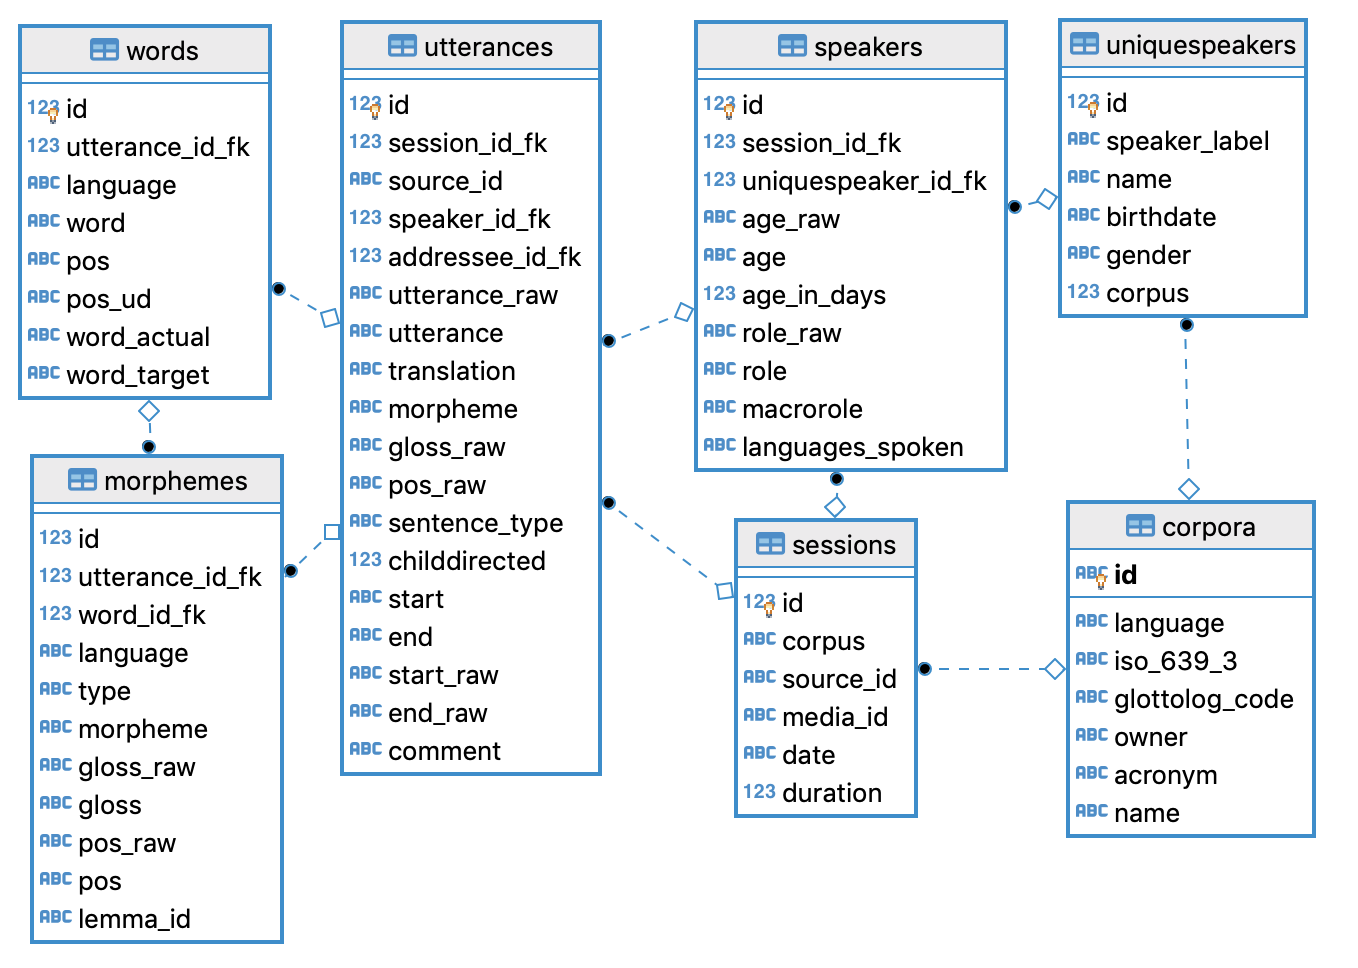
\includegraphics[scale=0.6]{pics/acqdiv-schema.png}
	\caption{Entity-relationship diagram of the ACQDIV Corpus Database}
	\label{fig:Entity-relationship diagram of the ACQDIV Corpus Database}
\end{figure}


\begin{comment}
Joining information from several tables requires a key field with shared values. Currently, composite keys have to be used in all relevant cases, i.e.\ the link between tables has to be established by several fields as follows: 

\begin{itemize}
	\item The tables \texttt{utterances} and \texttt{sessions} are linked via the combination of the fields \texttt{corpus} and \texttt{session\und id(\und fk)}.  
		The composite key is required because session IDs may not be unique across corpora. 
	\item The tables \texttt{utterances} and \texttt{speakers} are linked via the combination of the fields \texttt{corpus}, \texttt{session\und id(\und fk)}, 
		and \texttt{speaker\und label}. The composite key is required because speaker labels may not be unique across corpora and because age and roles 
		can change with the session. 
	\item The tables \texttt{words} (or \texttt{morphemes}) and \texttt{utterances} are linked via the combination of the fields \texttt{corpus} and 
		\texttt{utterance\und id(\und fk)}. The composite key is required because utterance IDs may not be unique across corpora. 
\end{itemize}


\begin{landscape}
\begin{figure}
	\centering
	\includegraphics[scale=0.6]{pics/ERD.png}
	\caption{Entity-relationship diagram of the ACQDIV Corpus Database}
	\label{fig:Entity-relationship diagram of the ACQDIV Corpus Database}
\end{figure}
\end{landscape}
\end{comment}

\noindent The following subsections explain the ACQDIV Corpus Database's tables' contents and where the data in these fields originate, i.e.\ from the original input corpus data (``data'') or in our ACQDIV Corpus Database Pipeline aggregation tool (``postprocessing'').\footnote{\url{https://github.com/acqdiv/acqdiv}} For more detail information on data aggregation, see Section \ref{sec:Building the database and postprocessing}).

% TODO: remove all mentions of postprocessing?

\subsection{Table \texttt{corpora}}
\label{subsec:Table corpora}

\begin{longtable}{lp{.5\linewidth}p{.2\linewidth}}
	\toprule
		\textbf{Column} & \textbf{Content} 	& \textbf{Origin} \\
	\midrule
	\endhead
		
	\bottomrule\\[-0.15cm]
	\caption{Columns of the table \texttt{corpora}}
	\endfoot

		\texttt{id} & an ID for the corpus & postprocessing \\
		\texttt{language} & language name & postprocessing \\
		\texttt{iso\_639\_3} & ISO 639-3 language name identifier & postprocessing \\
		\texttt{glottolog\_code} & Glottolog glottocode & postprocessing \\
		\texttt{owner} & name of the corpus owner & postprocessing \\
		\texttt{acronym} & acronym for the corpus & postprocessing \\
		\texttt{name} & name of the corpus & postprocessing \\
		\label{tab:Table corpora}
\end{longtable}


\subsection{Table \texttt{sessions}}
\label{subsec:Table sessions}

\begin{longtable}{lp{.5\linewidth}p{.2\linewidth}}
	\toprule
		\textbf{Column} & \textbf{Content} 	& \textbf{Origin} \\
	\midrule
	\endhead
		
	\bottomrule\\[-0.15cm]
	\caption{Columns of the table \texttt{session}}
	\endfoot
	
	
		\texttt{id}				& an automatically generated numeric ID for the session & postprocessing \\
		\texttt{corpus}			& the name of the corpus the session belongs to & data \\
		\texttt{source\und id}	& the name of the transcript file associated with the session. Note that source IDs are sometimes not unique across all corpora, so they are of limited use for identifying sessions. & data \\
		\texttt{media\und id}	& the id of the associated media (if available) & data \\

		% \texttt{language}		& the language of the corpus. While normally one language corresponds to one corpus, some languages may be represented by several corpora & postprocessing \\
		\texttt{date} 			& the recording date for the session & data \\ 
		\texttt{duration} 			& the recording sessions duration (if available) & postprocessing \\ 
		% \texttt{target\und child\und fk}  & the unique ID of the target child of the session, linking to the table \texttt{uniquespeakers} & postprocessing \\ 
		% \texttt{situation} 		& informal notes on the situation at the time of recording & data \\
		% \texttt{genre} 			& the genre of the recording & data \\ it, right?
		% \texttt{media} 			& the file name of the associated primary media file & data \\
		% \texttt{media\und type} & the type of the associated primary media file (mostly video, sometimes audio) & data \\[-0.3cm]
		\label{tab:Table sessions}
\end{longtable}


\subsection{Table \texttt{speakers}}
\label{subsec:Table speakers}

\begin{longtable}{lp{.5\linewidth}p{.2\linewidth}}
	\toprule
		\textbf{Column} & \textbf{Content} 	& \textbf{Origin} \\
	\midrule
	\endhead
	
	\bottomrule\\[-0.15cm]
	\caption{Columns of the table \texttt{speakers}}
	\endfoot
	
		\texttt{id}				& an automatically generated numeric ID for the speaker-session combination & postprocessing \\
		\texttt{session\und id\und fk} & the ID of the session the speaker appeared in, linking to the table \texttt{session} & data \\
		\texttt{uniquespeaker\und id\und fk} & the unique ID of the speaker independently of sessions, linking to the table \texttt{uniquespeakers} & postprocessing \\
		\texttt{age\und raw} 	& the age as given in the original data. This may be formally slightly different from the standardized form given in \texttt{age} & data \\
		\texttt{age} 			& the age of the speaker at the time when the current session was recorded. The age may be given in years or (especially for children) in the formats Y;M.D or Y;M & postprocessing \\
		\texttt{age\und in\und days} & the equivalent of the age in days & postprocessing \\
		\texttt{role\und raw} 	& the role as given in the original data. This is often slightly different from the standardized form in 
		\texttt{role} because of terminological differences (“target child” vs.\ “focus child” etc.) & data \\
		\texttt{macrorole} 		& this column only allows four values: Target\und Child, Child (any other children younger than or 12 years old),  Adult (older than 12 years), Unknown. Its purpose is to make the most basic age- and role-related information available for all speakers, even when the precise age and/or role are not known. & postprocessing \\
		\texttt{languages\und spoken} & a space-separated list of all languages the speaker is able speak, given in the form of ISO 639-2 codes & data \\\begin{comment}		
		\texttt{corpus}			& the name of the corpus the utterance belongs to & data \\
		\texttt{language}		& the language of the corpus & postprocessing \\
		\texttt{speaker\und label} & a code used to identify the speaker within the current corpus & data \\
		\texttt{name} 			& the full name of the speaker & data \\

		\texttt{gender} 		& the gender of the speaker. The only allowed values are “female” and “male”. & postprocessing \\
		\texttt{gender\und raw} & the gender as given in the original data, sometimes slightly different from the processed form & data \\
		\texttt{role} 			& the role performed by the speaker in the present recording. Because of the diversity of the ACQ\-DIV corpora, 
			 					  this concept covers both kinship terms (given in relation to the target child) and roles related to the 
								  setting (e.g.\ speaker, recorder, assistant). See \hyperref[subsec:Roles and macroroles]{below} for 
								  a list of the possible values of this field. & postprocessing \\

		\texttt{birthdate} 		& the birthdate of the speaker in the format YYYY-MM-DD & data \\[-0.3cm] 
\end{comment}
	\label{tab:Table speakers}
\end{longtable}


\subsection{Table \texttt{uniquespeakers}}
\label{subsec:Table uniquespeakers}

The corpora themselves do not always make it clear which of the speaker labels they use are unique, so this table requires some additional explanation. 
In the CHAT-based corpora, different speakers with identical speaker labels occur regularly because (different) target children always have the code CHI and their mothers are always referred to as MOT. Thus, speaker labels alone are not sufficient for identifying unique speakers. The \texttt{uniquespeakers} table therefore uses unique combinations of speaker labels, full names, and birthdates (if available) to achieve this. % SM: is "corpus" actually included in the logic? Birthdate is often "Unknown", so we fall back to code+name for less important speakers; couldn't they be ambiguous across corpora? -> nope, not included

On the other hand, there is also the less frequent case of a single speaker being referred to by different labels (and/or names and birthdates) because of gaps or mistakes in the metadata. These case are currently ignored, i.e.\ these cases may appear as different speakers in the \texttt{uniquespeakers} table. 

\begin{longtable}{lp{.5\linewidth}p{.2\linewidth}}
	\toprule
		\textbf{Column} & \textbf{Content} 	& \textbf{Origin} \\
	\midrule
	\endhead
	
	\bottomrule\\[-0.15cm]
	\caption{Columns of the table \texttt{uniquespeaker}}
	\endfoot
	
		\texttt{id} 		& an automatically generated numeric ID for the speaker & postprocessing \\
		\texttt{speaker\und label} & a code used to identify the speaker within the associated corpus & data \\
		\texttt{name}		& the full name of the speaker & data \\
		\texttt{birthdate} 	& the birthdate of the speaker in the format YYYY-MM-DD & data \\ 
		\texttt{gender} 	& the gender of the speaker & postprocessing \\
		\texttt{corpus} 	& the corpus the speaker appears in & data \\ [-0.3cm]
	\label{tab:Table uniquespeakers}
\end{longtable}


\subsection{Table \texttt{utterances}}
\label{subsec:Table utterances}

\begin{longtable}{lp{.5\linewidth}p{.2\linewidth}}
	\toprule
		\textbf{Column} & \textbf{Content} 	& \textbf{Origin} \\
	\midrule
	\endhead
	
	\bottomrule\\[-0.15cm]
	\caption{Columns of the table \texttt{utterance}}
	\endfoot

		\texttt{id}				& an automatically generated numeric ID for the utterance & postprocessing \\
		\texttt{session\und id\und fk} & the ID of the session the utterance belongs to, linking to the table \texttt{session} & data \\
		\texttt{source\und id} 	& the ID of the utterance in the original data & data \\
		\texttt{speaker\und id\und fk} & the ID of the speaker who produced the utterance, linking to the table \texttt{speakers} & postprocessing \\
		\texttt{addressee\_id\_fk}		& the ID of the addressee (when available) \\
		\texttt{utterance\und raw} & the original orthographic representation of an utterance (created by concatenating the single words if no separate representation is available &  \\ 
		\texttt{utterance}		& an orthographic representation of the utterance (created by concatenating the single words if no separate representation is available; cleaned of punctuation marks) & postprocessing \\
		\texttt{translation}	& a free translation of the utterance (mostly English but Spanish for Yucatec) & data \\
		\texttt{morpheme}		& all morphemes contained in an utterance, separated by spaces (concatenated morphemes) & postprocessing \\
		\texttt{gloss\und raw}  & all glosses contained in an utterance, separated by spaces (concatenated morphemes) & postprocessing  \\
		\texttt{pos\und raw}	& all part-of-speech tags contained in an utterance, separated by spaces (concatenated morphemes) & postprocessing \\
		\texttt{sentence\und type} &	broad sentence types, the most frequent values being \texttt{default}, \texttt{question} and \texttt{exclamation}. This may be taken directly from the data or inferred on the base of sentence delimiters. & data or postprocessing \\
		\texttt{childdirected} & \texttt{1} for utterances directed to a target child, \texttt{0} for all others (including unknown addressees) & data or postprocessing \\
		\texttt{start}			& the point in time in an associated media file where the utterance starts; format HH:MM:SS. & postprocessing \\ 
		\texttt{end}			& the point in time in an associated media file where the utterance ends; format HH:MM:SS. & postprocessing \\
		\texttt{start\und raw} 	& like \texttt{start} but not unified to HH:MM:SS & data \\		
		\texttt{end\und raw}	& like \texttt{end} but not unified to HH:MM:SS & data \\
		\texttt{comment}		& any comments on the utterance. This tier merges several tiers that are separated in some of the subcorpora  but mostly overlap due to inconsistent usage: actions accompanying an utterance, background situation, ethnographic comments, comments on grammar, generic comments. & data \\

		\begin{comment}
		\texttt{uniquespeaker\und id\und fk} & the ID of the \hyperref[subsec:Table uniquespeakers]{unique speaker} who produced the utterance, linking to the table \texttt{uniquespeakers} & postprocessing \\
		\texttt{speaker\und label} & a code which uniquely identifies the speaker of an utterance within a corpus and presents a link to the tables \texttt{speaker} and \texttt{uniquespeaker} & data \\

		% \texttt{phonetic}		& a phonetic transcription of the actual utterance, mostly in IPA & data \\ % only four corpora have this: Chintang, Cree, Indonesian, Yucatec
		\end{comment}
					
	\label{tab:Table utterances}
\end{longtable}

% List of obsolete tiers/columns

% \item \textbf{argument_coding:} various types of syntactic coding. This tier is presently not passed on from JSON to R because it is only present in a few corpora.
% \item \textbf{error\und coding:} free coding of errors made by children. This tier is presently not passed on from JSON to R because it is only present in a few corpora.
% \item \textbf{gestures:} free coding of gestures accompanying speech. This tier is presently not passed on from JSON to R because it is only present in a few corpora.
% \item \textbf{information_structure:} free coding of information structure. This tier is presently not passed on from JSON to R because it is only present in a few corpora.
% \item \textbf{nepali:} a free Nepali translation of the utterance
% \item \textbf{spanish:} a free Spanish translation of the utterance
% \item \textbf{syntax\und coding:} various types of syntactic coding. This tier is presently not passed on from JSON to R because it is only present in a few corpora.

The table below shows which of the utterance columns are regularly filled in which of the corpora. 

% \small
\begin{longtable}{lccccccccccc}	
	% \toprule
	\textbf{tier} 				& \rot{\textbf{CLC} (ctn)} & \rot{\textbf{CCLAS} (crl)} & \rot{\textbf{JCLD} (ind)} & \rot{\textbf{AIC} (ike)} & \rot{\textbf{MPJC} (jpn)} & \rot{\textbf{MYJC} (jpn)} & \rot{\textbf{StRuC} (rus)} & \rot{\textbf{DSC} (sot)} & \rot{\textbf{KULLDD} (tur)} & \rot{\textbf{PYC} (yua)} & \rot{\textbf{SNC} (yuw)}\\
	\midrule
	\endhead
	
	\bottomrule\\[-0.15cm]
	\caption{Presence of columns in the table \texttt{utterances}}
	\endfoot
	
	\small
	
	addressee 					&  (+) 		& - 	& - 		& + 		 & (+) 	  & (+) 	& -    	 & -  		& + 	  & - 	 & -  \\
%	argument\und coding 		&  - 		& - 	& - 		& +  		 & - 	  & -  		& - 	 & -  		& - 	  & - 	 & -  \\
	childdirected 				&  (+) 		& - 	& - 		& +  		 & + 	  & +  		& - 	 & -  		& + 	  & - 	 & -  \\
	comment 					&  + 		& + 	& + 		& +  		 & + 	  & +  		& + 	 & +  		& + 	  & + 	 & +  \\
	corpus	 					&  + 		& + 	& +  		& +  		 & + 	  & +  		& + 	 & +  		& + 	  & + 	 & +  \\
	end	 						&  + 		& + 	& - 		& -  		 & + 	  & (+)  	& (+) 	 & +  		& - 	  & - 	 & +  \\
	end\und raw	 				&  + 		& + 	& - 		& -  		 & + 	  & (+)  	& (+) 	 & +  		& - 	  & - 	 & +  \\
%	error\und coding 			&  - 		& - 	& - 		& +  		 & - 	  & +  		& - 	 & -  		& + 	  & - 	 & -  \\
	% gestures 					&  - 		& - 	& - 		& -  		 & - 	  & +  		& - 	 & -  		& + 	  & - 	 & -  \\
	id		 					&  + 		& + 	& +  		& +  		 & + 	  & +  		& + 	 & +  		& + 	  & + 	 & +  \\
%	information\und structure 	&  - 		& - 	& -  		& -  		 & + 	  & -  		& - 	 & -  		& - 	  & - 	 & -  \\
%	orthographic 				&  - 		& - 	& -  		& -  		 & + 	  & +  		& - 	 & -  		& - 	  & - 	 & -  \\
	language					&  + 		& + 	& +  		& +  		 & + 	  & +  		& + 	 & +  		& + 	  & + 	 & +  \\
%	phonetic 					&  - 		& + 	& +  		& -  		 & - 	  & -  		& + 	 & -  		& - 	  & + 	 & +  \\
	sentence\und type 			&  - 		& + 	& -  		& +  		 & + 	  & +  		& - 	 & +  		& + 	  & + 	 & +  \\
	speaker\und label 			&  + 		& + 	& +  		& +  		 & + 	  & +  		& + 	 & +  		& + 	  & + 	 & +  \\
	session\und id\und fk	 	&  + 		& + 	& +  		& +  		 & + 	  & +  		& + 	 & +  		& + 	  & + 	 & +  \\
	start		 				&  + 		& + 	& +  		& +  		 & + 	  & (+)  	& (+) 	 & +  		& - 	  & - 	 & +  \\
	start\und raw 				&  + 		& + 	& +  		& +  		 & + 	  & (+) 	& (+) 	 & +  		& - 	  & - 	 & +  \\
%	syntax\und coding 			&  - 		& - 	& -  		& +  		 & - 	  & -  		& - 	 & -  		& - 	  & - 	 & -  \\
	translation					&  + 		& + 	& + 		& +  		 & - 	  & -  		& - 	 & +  		& + 	  & + 	 & +  \\
	uniquespeaker\und id\und fk &  + 		& + 	& +  		& +  		 & + 	  & +  		& + 	 & +  		& + 	  & + 	 & +  \\
	utterance		 			&  + 		& + 	& +  		& +  		 & + 	  & +  		& + 	 & +  		& + 	  & + 	 & +  \\
	utterance\und id 			&  + 		& + 	& +  		& +  		 & + 	  & +  		& + 	 & +  		& + 	  & + 	 & +  \\
	utterance\und raw 			&  + 		& + 	& +  		& +  		 & + 	  & +  		& + 	 & +  		& + 	  & + 	 & +  \\
	warning 					&  + 		& + 	& + 		& + 		 & + 	  & + 		& + 	 & + 		& + 	  & + 	 & +  \\
\end{longtable}

\subsection{Table \texttt{words}}
\label{subsec:Table words}

\begin{longtable}{lp{.5\linewidth}p{.2\linewidth}}
	\toprule
		\textbf{Column} & \textbf{Content} 	& \textbf{Origin} \\
	\midrule
	\endhead
	
	\bottomrule\\[-0.15cm]
	\caption{Columns of the table \texttt{words}}
	\endfoot
	
		\texttt{id} & an automatically generated numeric ID for the word & postprocessing \\
		\texttt{utterance\und id\und fk} & the ID of the utterance the word belongs to, linking to the table \texttt{utterances} & data \\
		% \texttt{session\und id\und fk} & the ID of the session the word belongs to, linking to the table \texttt{sessions} & data \\
		% \texttt{corpus} 			& the name of the corpus the word belongs to & data \\ 
		% \texttt{language}			& the language of the corpus & postprocessing \\
		\texttt{language}	& the language of the stem of a word; equals the corpus language by default & data \\							  
		\texttt{word}				& an orthographic representation of a word. When both actual and target forms are available 
									  (see \autoref{subsec:Actual and target fields}), this is the actual word; otherwise it is the only available form. 
									  See \texttt{word\und actual} and \texttt{word\und target} for more precisely specified (but often empty) word forms. & data \\
		\texttt{pos}				& the standardized part-of-speech tag of the stem of the word & postprocessing \\
		\texttt{pos\und ud}       &  the universal part-of-speech tag\footnote{\url{http://universaldependencies.org/u/pos/}} of the stem of the word & postprocessing \\
		\texttt{word\und actual}	& the word form the speaker actually produced; may be empty when only the target form is known & data \\
		\texttt{word\und target}	& the word form the speaker intended to produce; may be empty when only the actual form is known & data \\
	\label{tab:Table words}
\end{longtable}

The table below shows which of these columns are regularly filled in which of the corpora. 

% \small
\begin{longtable}{lccccccccccc}	
	% \toprule
	\textbf{tier} 				& \rot{\textbf{CLC} (ctn)} & \rot{\textbf{CCLAS} (crl)} & \rot{\textbf{JCLD} (ind)} & \rot{\textbf{AIC} (ike)} & \rot{\textbf{MPJC} (jpn)} & \rot{\textbf{MYJC} (jpn)} & \rot{\textbf{StRuC} (rus)} & \rot{\textbf{DSC} (sot)} & \rot{\textbf{KULLDD} (tur)} & \rot{\textbf{PYC} (yua)} & \rot{\textbf{SNC} (yuw)}\\
	\midrule
	\endhead
	
	\bottomrule\\[-0.15cm]
	\caption{Presence of columns in the table \texttt{words}}
	\endfoot
	
	corpus						&  + 		& + 	& +  		& +  		 & + 	  & +  		& + 	 & +  		& + 	  & + 	 & + \\
	id		 					&  + 		& + 	& +  		& +  		 & + 	  & +  		& + 	 & +  		& + 	  & + 	 & + \\
	language					&  + 		& + 	& +  		& +  		 & + 	  & +  		& + 	 & +  		& + 	  & + 	 & + \\
	session\und id\und fk		&  + 		& + 	& +  		& +  		 & + 	  & +  		& + 	 & +  		& + 	  & + 	 & + \\
	utterance\und id\und fk		&  + 		& + 	& +  		& +  		 & + 	  & +  		& + 	 & +  		& + 	  & + 	 & + \\
	warning 					&  + 		& + 	& + 		& + 		 & + 	  & + 		& + 	 & + 		& + 	  & + 	 & + \\
	word	 					&  + 		& + 	& +  		& +  		 & + 	  & +  		& + 	 & +  		& + 	  & + 	 & + \\
	word\und actual 			&  + 		& + 	& + 		& +  		 & + 	  & +  		& + 	 & +  		& + 	  & (+)  & - \\
	word\und target 			&  - 		& + 	& + 		& +  		 & + 	  & +  		& - 	 & +  		& + 	  & + 	 & + \\
	pos 						&  + 		& + 	& (+)  		& +  		 & + 	  & +  		& + 	 & +  		& + 	  & +    & + \\
        pos\und ud 						&  + 		& + 	& (+)  		& +  		 & + 	  & +  		& + 	 & +  		& + 	  & +    & + \\

\end{longtable}
\normalsize

\subsection{Table \texttt{morphemes}}
\label{subsec:Table morphemes}


\begin{longtable}{lp{.5\linewidth}p{.2\linewidth}}
	\toprule
		\textbf{Column} & \textbf{Content} 	& \textbf{Origin} \\
	\midrule
	\endhead
	
	\bottomrule\\[-0.15cm]
	\caption{Columns of the table \texttt{morphemes}}
	\endfoot

		\texttt{id}	 			& an automatically generated numeric ID for the morpheme & postprocessing \\
		\texttt{utterance\und id\und fk} & the ID of the utterance the morpheme belongs to, linking to the table \texttt{utterances} & data \\		
		\texttt{word\und id\und fk} & the ID of the word the morpheme belongs to, linking to the table \texttt{words} & data \\ 
		\texttt{language}	& the language of an individual morpheme; equals the corpus language by default & data \\
		\texttt{type} 			& the morpheme type (actual vs.\ target, (see \autoref{subsec:Actual and target fields}). Because most corpora only
								  specify either the actual or the target morpheme most of the time (differently from the word level, where contrasting forms are often given), only this one form is taken over and the type is specified in this column. & data \\
		\texttt{morpheme} 		& an orthographic representation of a morpheme (often in its underlying shape). Mostly this is the only form available, but in the rare case where both an actual and a target form are given only the actual form is taken over. \\
		\texttt{gloss\und raw} 	& the original gloss (before standardization). Depending on the corpus, this column may contain glosses for both grammatical and lexical morphemes (differently from \texttt{gloss}, where only standardized grammatical labels appear). & data \\
		\texttt{gloss} 			& a standardized label indicating the function of grammatical morphemes. The \href{http://www.eva.mpg.de/lingua/resources/glossing-rules.php}{Leipzig Glossing Rules} form the base for standardization and additional labels are drawn from a project-internal vocabulary given in \autoref{subsec:Grammatical glosses}. Morphemes whose original form cannot be assigned to a standard appear as \texttt{\textsc{null}} in this column. This also includes all lexical morphemes \textendash\ there are too many different types in this partition to create a standardized vocabulary, and there are no simple automatizable rules for distinguishing them from grammatical morphemes. & data/postprocessing \\
		\texttt{pos\und raw} 	& the original part-of-speech tag (before standardization) & data \\		
		\texttt{pos} 			& a part-of-speech tag. Parts of speech are also standardized. The project-internal set of tags is given in \autoref{subsec:Part-of-speech tags} & data/postprocessing \\
		\texttt{lemma\_id} 		& the lemma dictionary ID (only available for Chintang) & postprocessing \\

	\label{tab:Table morphemes}
\end{longtable}

The table below shows which of these columns are regularly filled in which of the corpora. 

% \small
\begin{longtable}{lccccccccccc}	
	% \toprule
	\textbf{tier} 				& \rot{\textbf{CLC} (ctn)} & \rot{\textbf{crl} (CCLAS)} & \rot{\textbf{JCLD} (ind)} & \rot{\textbf{AIC} (ike)} & \rot{\textbf{MPJC} (jpn)} & \rot{\textbf{MYJC} (jpn)} & \rot{\textbf{StRuC} (rus)} & \rot{\textbf{DSC} (sot)} & \rot{\textbf{KULLDD} (tur)} & \rot{\textbf{PYC} (yua)} & \rot{\textbf{SNC} (yuw)}\\
	\midrule
	\endhead
	
	\bottomrule\\[-0.15cm]
	\caption{Presence of columns in the table \texttt{morphemes}}
	\endfoot
	
	corpus						&  + 		& + 	& +  		& +  		 & + 	  & +  		& + 	 & +  		& + 	  & + 	  & + 	 \\
	language					&  + 		& + 	& +  		& +  		 & + 	  & +  		& + 	 & +  		& + 	  & + 	  & + 	 \\
	gloss	 					&  + 		& + 	& +  		& +  		 & (+) 	  & (+)		& + 	 & +  		& (+) 	  & (+)   & +   \\
	gloss\und raw	 			&  + 		& + 	& +  		& +  		 & (+) 	  & (+)		& + 	 & +  		& + 	  & + 	  & + 	 \\
	id		 					&  + 		& + 	& +  		& +  		 & + 	  & +  		& + 	 & +  		& + 	  & + 	  & + 	 \\
	language					&  + 		& + 	& +  		& +  		 & + 	  & +  		& + 	 & +  		& + 	  & + 	  & + 	 \\
	morpheme\und language		&  + 		& + 	& -  		& -  		 & + 	  & +  		& + 	 & -  		& + 	  & - 	  & + 	 \\
	morpheme 					&  + 		& + 	& +  		& +  		 & (+) 	  & (+)		& + 	 & +  		& (+) 	  & +  	  & +  	 \\
	pos 						&  + 		& + 	& (+)  		& +  		 & + 	  & +  		& + 	 & +  		& + 	  & +  	  & +  	 \\
	pos\und raw 				&  + 		& + 	& -  		& +  		 & + 	  & +  		& + 	 & +  		& + 	  & +  	  & +  	 \\
	session\und id\und fk		&  + 		& + 	& +  		& +  		 & + 	  & +  		& + 	 & +  		& + 	  & + 	  & + 	 \\
	type						&  + 		& + 	& +  		& +  		 & + 	  & +  		& + 	 & +  		& + 	  & + 	  & + 	 \\
	utterance\und id\und fk		&  + 		& + 	& +  		& +  		 & + 	  & +  		& + 	 & +  		& + 	  & + 	  & + 	 \\
	warning 					&  + 		& + 	& + 		& + 		 & + 	  & + 		& + 	 & + 		& + 	  & + 	  & + 	 \\

\end{longtable}
\normalsize


\subsection{Table \texttt{all\und data} (view)}
\label{subsec:Table all_data}

This table view that is generated by joining and denormalizing all of the tables mentioned above. IDs and foreign keys on which the merger is performed, duplicated columns, and a few less often used columns are omitted. Some columns are renamed in order to make clear which table they originate from, e.g.\ utterance\_id. 

When using the \texttt{all\und data} view, it is critical to understand that many of the \texttt{morpheme} and \texttt{word} fields are \texttt{NULL}. This is due to a decision by developers to keep both the word and morpheme tiers \textbf{even when they do not align correctly in the input data}. This allows users to use the word, morpheme, gloss, etc., tiers independently without throwing out all data that does not align. Unfortunately, the input corpora are quite problematic, and as such, there are many misalignments.

\begin{comment}
The table below shows the correspondences between original columns and columns in \texttt{all\und data}. 

\begin{longtable}[ht!]{lll}
	\toprule
		\textbf{original table} & \textbf{old column} & \textbf{new column} \\
	\midrule
	\endhead
	
	\bottomrule\\[-0.15cm]
	\caption{Columns in the merged table}
	\endfoot
	
		sessions 				& id					& session\und id \\
		sessions 				& source\und id			& session\und id\und source \\
		sessions 				& corpus				& corpus \\
		sessions 				& language				& language \\
		sessions 				& date					& date \\
		% sessions 				& media					& - \\
		% sessions 				& media\und type 		& - \\
		speakers				& id 					& speaker\und id \\
		speakers				& uniquespeaker\und id\und fk 	& - \\
		speakers				& session\und id 		& - \\
		speakers				& corpus				& corpus \\
		speakers				& language				& language \\
		speakers				& speaker\und label 	& speaker\und label \\
		speakers				& name					& name \\
		speakers				& age					& age \\
		speakers				& age\und in\und days 	& age\und in\und days \\
		speakers				& age\und raw			& age\und raw \\
		speakers				& gender 				& gender \\
		speakers				& gender\und raw		& gender\und raw \\
		speakers				& role					& role \\
		speakers				& macrorole				& macrorole \\
		speakers				& role\und raw			& role\und raw \\
		speakers				& languages\und spoken 	& - \\
		speakers				& birthdate				& birthdate \\
		uniquespeakers 			& id					& - \\
		uniquespeakers 			& speaker\und label		& - \\
		uniquespeakers 			& corpus				& - \\
		uniquespeakers 			& name					& - \\
		uniquespeakers 			& birthdate				& - \\
		uniquespeakers 			& gender				& - \\			
		utterances				& id					& utterance\und id \\
		utterances				& session\und id\und fk	& - \\
		utterances				& source\und id			& utterance\und id\und source \\
		utterances				& corpus				& corpus \\
		utterances				& language				& language \\
		utterances				& speaker\und label		& speaker\und label \\
		utterances				& addressee				& addressee \\
		utterances				& utterance				& utterance \\
		utterances				& utterance\und raw		& utterance\und raw \\
		utterances				& translation			& translation \\
		utterances				& sentence\und type		& sentence\und type \\
		utterances				& start					& start \\
		utterances				& start\und raw			& start\und raw \\
		utterances				& end					& end \\
		utterances				& end\und raw			& end\und raw \\
		utterances				& morpheme				& utterance\und morphemes \\
		utterances				& gloss\und raw			& utterance\und glosses\und raw \\
		utterances				& pos\und raw			& utterance\und poses\und raw \\
		utterances				& comment				& comment \\
		utterances				& warning				& - \\
		words					& id					& word\und id \\
		words					& utterance\und id\und fk & - \\
		words					& session\und id\und fk	& - \\
		words					& corpus				& corpus \\
		words					& language				& language \\
		words					& word					& word \\
		words					& word\und actual		& word\und actual \\
		words					& word\und target		& word\und target \\
		words					& pos					& pos\und word\und stem \\
		words					& warning				& - \\
		morphemes				& id					& morpheme\und id \\
		morphemes				& word\und id\und fk	& - \\
		morphemes				& utterance\und id\und fk & - \\
		morphemes				& session\und id\und fk & - \\
		morphemes				& corpus				& corpus \\
		morphemes				& language				& language \\
		morphemes				& type					& morpheme\und type \\
		morphemes				& morpheme				& morpheme \\
		morphemes				& gloss					& gloss \\
		morphemes				& gloss\und raw			& gloss\und raw \\
		morphemes				& pos					& pos \\
		morphemes				& pos\und raw			& pos\und raw \\
		morphemes				& warning				& - \\

		\label{tab:Columns in the merged table}
\end{longtable}
\end{comment}

\subsection{Actual and target fields}
\label{subsec:Actual and target fields}

All of the original subcorpora make a distinction between what a child actually said and what the adult target form would have been. Although none of the corpora carries this distinction through on all tiers of all levels, all of them incorporate it at least implicitly and many have separate tiers for the actual and target versions of at least overarching tiers. The table below shows for each corpus if the main tiers of each level always belong to one type (“a(ctual)” or “t(arget)”), if the types are distinguished using separate tiers (“a vs.\ t”), or if both types are mixed on a single tier without making a clear distinction (“a/t”).

% TODO: update tables with new languages
\begin{table}[ht!]
	\centering
	\begin{tabular}{lllll}
		\toprule
			\textbf{subcorpus} & \texttt{words} & \texttt{morphemes} 	& \texttt{morphemes} & \texttt{morphemes} \\
							   & \texttt{word}  & \texttt{morpheme} 	& \texttt{gloss} 	 & \texttt{pos} \\
		\midrule
			CLC	(Chintang) 		   & a			  	 & t					& t			 		& t     \\
			CCLAS (Cree)		   & a vs.\ t		 & a vs.\ t				& t			 		& t	  	\\
			JCLD (Indonesian)	 	   & a vs.\ t		 & t					& t			 		& - 	\\
			AIC	(Inuktitut)		   & a vs.\ t		 & t/a					& t			 		& t  	\\
			MPJC (Japanese)		   & a vs.\ t		 & t/a					& t/a			 	& t/a 	\\
			MYJC (Japanese)		   & a vs.\ t 	  	 & t		 			& t			 		& t	  	\\
			StRuC (Russian)		   & a			  	 & t					& t			 		& t	  	\\
			DSC	(Sesotho)		   & a vs.\ t		 & t	 				& t			 		& t 	\\
			KULLDD (Turkish)	   & a vs.\ t 	  	 & t/a					& t/a		 		& t/a	\\
			PYC	(Yucatec)		   & t/a			 & t					& t			 		& t	  	\\
			SNC	(Nungon)		   & t			  	 & t					& t			 		& t	  	\\
		\bottomrule
	\end{tabular}
	\caption{Actual and target tiers in the original subcorpora}
	\label{tab:Actual and target tiers in the original subcorpora}
\end{table}

Since there is not a single corpus which consistently codes the actual/target distinction on all tiers of all levels and the overall emerging picture is rather chaotic, the following rules for simplification were applied: 

\begin{itemize}
	\item The distinction is most relevant and most frequently coded on the word level. Therefore, the \texttt{words} table of the ACQDIV Corpus Database
		features three columns: \texttt{word\und actual}, \texttt{word\und target}, and \texttt{word}. The latter is intended for easy searches
		regardless of the actual/target distinction. It contains the actual word form by default but may contain the target word form in the rare
		case that the actual word form is not available.
	\item On the morpheme level, the actual/target distinction is less relevant and less consistently coded. The \texttt{morphemes} table
		therefore only gives three default columns (\texttt{morpheme}, \texttt{gloss}, \texttt{pos}) and an additional column \texttt{type}
		that specifies if the values normally correspond to actual or to target forms. This representation glosses over inconsistencies (many of the subcorpora 
		do not have a clear guideline for the distinction on the morpheme level so that both actual and target forms are found) and ignores any 
		differences that might exist between the three fields. 
	\item Finally, only two corpora (Cree and Indonesian) makes a distinction on the utterance level. This distinction is therefore completely ignored in the ACQDIV Corpus Database. 
\end{itemize}

% This is described in detail in issue #609.
% We no longer use this field (consistent\_actual\_target)
\begin{comment}
The current implementation for \texttt{word\und actual} and \texttt{word\und target} is encoded with a binary value in the \textit{consistent\_actual\_target} field in the corpus-specific configuration files. The reasoning behind this decision is that if a corpus has a high congruence between actual and target in child speech, it is likely, that the transcribers/annotators did not make the distinction consistently. In other words, ``inconsistently coded" means there are some cases where an actual/target distinction has been coded but they are so few that it's very unlikely that the coding is consistent. There are two corpora that are currently tagged \textit{consistent\_actual\_target$==$no}. These are Yucatec and Nungon. In Yucatec, the transcription comes on three lines (Pfeiler, p.c.):

\begin{enumerate}
\item the expression according to the norm
\item phon: what the child actually said
\item eng/esp: Translation into Spanish.
\end{enumerate}

\noindent In our data processing, we did not include the CHAT \textit{\%(x)pho} tier, it being located on the utterance level (i.e.\ alignment to words is not guaranteed). All in all we had too few corpora with phonetic transcriptions on that level to introduce a column like \textit{utterances.phonetic}. Perhaps in Yucatec, however, the alignment is even good enough to pull at least the Yucatec tier to the word level -- evaluation pending. 

Regarding Nungon, the transcriber aims to write down the actual word spoken by the child (Sarvasy, p.c.). If the spoken form by the child diverges phonetically or phonologically from the adult enough to be noticed by the transcriber, this should be documented on the first tier. The second tier then reflects the target form, as understood by the transcriber. Large differences are noted by the transcriber, but minor ones may be missed (e.g.\ the child doesn't articulate a word medial syllable carefully). Hence Nungon given our criteria for inconsistent encoding is marked as ``no'', but this is due to the very few data points that we have and this issue should be revisited in the future when more data is put into the pipeline.

Finally, there is largely no difference in \textit{consistent\_actual\_target$==$yes} languages in the adult forms. That is, most transcriptions of words by adults are the same between actual spoken utterance and the target form. This seems a bit confusing from a database point-of-view, i.e.\ a lot of duplicated between two or three fields in the same table (word, word\_actual, word\_target). But the reasoning here is that each column can be taken separately depending on the analysis.
\end{comment}

\section{Conventions}
\label{sec:Conventions and standardization}

\subsection{Transcription conventions}
\label{subsec:Transcription conventions}

The transcription conventions used in the ACQDIV Corpus Database have been greatly simplified compared to the original subcorpora, especially those that were initially coded as CHAT or TalkBank XML. This was necessary in order to ensure maximal comparability. 

While the conventions for representing segmental material have not been touched, the following changes were applied with respect to additional symbols: 

\begin{itemize}
	\item All punctuation has been removed. The information contained in utterance delimiters (including CHAT’s Special Utterance Terminators) was transferred to the newly introduced tier \texttt{utterances.sentence\und type} (for instance, a utterance-final question mark now corresponds to the sentence type “question”). An exception is when is hyphens, e.g.\ he-eh, and underscores, e.g.\ ice\_cream. These exceptions are mainly low frequencies errors in the input data.
	\item All special CHAT codes such as postcodes, Satellite Markers, tone and prosody markers, quotation markers, Utterance Linkers, and overlap markers have been removed without replacement. 
	\item Likewise, CHAT’s Special Form Markers (codes starting with “@” attached to words) have been deleted. 
	\item CHAT’s Local Events have been transferred to the comment tier (concatenating them to any pre-existing material). Where the utterance only consists of an event, the sentence type has been set to “action”. Pauses, which are also classified as a special type of Local Event by the CHAT manual, have been removed without traces. 
	\item All types of codes for untranscribed material have been replaced by \texttt{NULL/NA} in isolation and by “???” when embedded into a string. This includes the CHAT codes “xxx”, “yyy”, “www”, so the the difference between unintelligible words, words with a clear phonetic shape but unclear phonology, and words not transcribed for other reasons is lost.
	\item Morpheme separators (mainly given on the morphology tiers, but sometimes also elsewhere) have been deleted. The information contained in them has been transferred to the field \texttt{morphemes.pos}, where all prefixes and suffixes get the dummy tags “pfx” and “sfx”, respectively. 
	\item A few corpora have explicit coding for compounds. This has been simplified (see the description of the \hyperref[cha:Data sources]{original data}), leaving only “=” as the separator between the compound elements (“apple=tree”). 
\end{itemize}

This leaves “???” (untranscribed element within string) and “=” (compound separator) as the only metalinguistic elements on the object language tiers. 

\subsection{Roles and macroroles}
\label{subsec:Roles and macroroles}

The ACQDIV Corpus Database currently allows the following values in the \texttt{speakers.role} field. This list is the result of a simplification of the values found in the original data, which are diverse both because of terminological differences (e.g.\ “target child” vs.\ “focus child”) and spelling mistakes (“Garndmother” vs.\ “Grandmother”). While some subcorpora distinguish between kinship terms (“mother”, “son”), age groups (“child”, “adult”), and other roles (“caretaker”, “playmate”) most of the corpora do not, so these categories also appear as one in the ACQDIV Corpus Database. 

\begin{multicols}{4}
	\noindent Adult \\
	Aunt \\
	Babysitter \\
	Boy \\
	Brother \\
	Caller \\
	Caretaker \\
	Child \\
	Cousin \\
	Daughter \\
	Family\und Friend \\
	Father \\
	Female \\
	Friend \\
	Girl \\
	Grandfather \\
	Grandmother \\
	Great-Grandmother \\
	Host \\
	Housekeeper \\
	Male \\
	Mother \\
	Neighbour \\
	Niece \\
	Playmate \\
	Research\und Team \\
	Sister \\
	Speaker \\
	Student \\
	Subject \\
	Target\und Child \\
	Teacher \\
	Teenager \\
	Toy \\
	Twin\und Brother \\
	Uncle \\
	Unknown \\
	Visitor \\
\end{multicols}

The field \texttt{speakers.macrorole}, which is created during postprocessing, is the result of mapping these roles to the four values “Child”, “Target\und Child”, “Adult”, and “Unknown”. Differently from the \texttt{role} field, macroroles also include inference based on age (younger than 12 years = “Child”) and IDs (e.g.\ CHI = “Child”; other ID-based mappings depend on the individual corpora). 


\subsection{Grammatical glosses}
\label{subsec:Grammatical glosses}

The ACQDIV Corpus Database uses a standardized set of grammatical glosses in the column \texttt{morphemes.gloss}. The value used in the original data is given in \texttt{morphemes.gloss\und raw}. The standardizet set consists of all glosses proposed in the \href{http://www.eva.mpg.de/lingua/resources/glossing-rules.php}{Leipzig Glossing Rules} plus additional values as needed (marked with an asterisk in the list below). Less frequent values were directly taken over from the original data in order to fill all rows but are not documented below. 

% original whitelist from integrity tests: 
% None, "0", "1", "1/2PL", "1DL", "1NSG", "1PL", "1SG", "2", "2DL", "NSG", "2SG", "2PL", "3", "3DL",
% "3NSG", "3SG", "3PL", "4", "4SYL", "A", "ABIL", "ABL", "ABS", "ACC", "ACROSS", "ACT", "ADESS", "ADJ",
% "ADJZ", "ADN", "ADV", "ADVZ", "AFF", "AGT", "AGR", "ALL", "ALT", "AMBUL", "ANIM", "ANTIP", "AOR",
% "APPL", "ART", "ASP", "ASS", "ASSOC", "ATTN", "AUTOBEN", "AUX", "AV", "BABBLE", "BEN", "CAUS", "CHOS",
% "CLF", "CLIT", "CM", "COM", "COMP", "COMPAR", "COMPL", "CONC", "COND", "CONJ", "CONJ", "CON", "CONT",
% "CONTEMP", "CONTING", "CONTR", "COP", "CVB", "DAT", "DECL", "DEF", "DEICT", "DEM", "DEP", "DEPR",
% "DESID", "DESTR", "DET", "DETR", "DIM", "DIR", "DIR", "DIST", "DISTR", "DOWN", "DU", "DUB", "DUR",
% "DYN", "ECHO", "EMPH", "EQU", "ERG", "EVID", "EXCL", "EXCLA", "EXIST", "EXT", "F", "FILLER", "FOC",
% "FUT", "FUT1", "GEN", "HAB", "HES", "HHON", "HON", "HORT", "I", "IDEOPH", "II", "III", "IMIT", "IMP",
% "IMPERS", "INAL", "INAN", "INCEP", "INCH", "INCL", "INCOMPL", "IND", "IND1", "IND2", "INDF", "INDIR",
% "INF", "INS", "INSIST", "INTJ", "INTR", "INTRG", "INV", "IPFV", "IRR", "IV", "IX", "LHON", "LNK",
% "LOC", "M", "MED", "MHON", "MIR", "MOD", "MOOD", "MV", "N", "N", "N", "NAG", "NAME", "NC", "NEG",
% "NICKNAMER", "NMLZ", "NOM", "NPST", "NSG", "NTVZ", "NUM", "OBJ", "OBJVZ", "OBL", "OBLIG", "OBV",
% "ONOM", "OPT", "ORD", "P", "PARTIT", "PASS", "PEJ", "PERL", "PERMIS", "PERSIST", "PFV", "PL", "POL",
% "POSS", "POT", "PRAG", "PRED", "PREDADJ", "PREP", "PREP", "PRF", "PRO", "PROB", "PROG", "PROH", "PROP",
% "PROX", "PRS", "PST", "PTCL", "PTCP", "PURP", "PV", "PVB", "Q", "QUANT", "QUOT", "RECENT", "RECNF",
% "RECP", "REF", "REFL", "REL", "REM", "REP", "RES", "REVERS", "S", "S/A", "S/P", "SBJ", "SBJV", "SEQ",
% "SG", "SIM", "SOC", "SPEC", "STAT", "STEM", "SUPERL", "SURP", "TEASER", "TEL", "TEMP", "TENSE", "TERM",
% "TOP", "TR", "UP", "V", "VI", "VII", "VIII", "V2", "V.AUX", "V.CAUS", "V.IMP", "V.ITR", "V.PASS",
% "V.POS", "V.TR", "VBZ", "VOICE", "VN", "VOC", "VOL", "WH", "X", "XI", "XII", "XII", "XIV", "???"
				 
\begin{multicols}{2}
	\begin{tabbing}
	*0 \hspace{2cm} \= non-person \\
	1 \> first person \\
	2 \> second person \\
	3 \> third person \\
	*4 \> fourth person (in switch refer-\\
		\> ence or direct/inverse systems) \\
	*4SYL \> tetrasyllabifier \\
	A \> agent-like argument of canon- \\
		\> ical transitive verb \\
	*ABIL \> abilitative \\
	ABL \> ablative \\
	ABS \> absolutive \\
	ACC \> accusative \\
	*ACROSS \> distal horizontal deixis \\
	*ACT \> active \\
	*ADESS \> adessive \\
	ADJ \> adjective \\
	*ADJZ \> adjectivizer \\
	*ADN \> adnominal \\
	ADV \> adverb(ial) \\
	*ADVZ \> adverbializer \\
	*AFF \> affirmative \\
	*AGT \> agentive \\
	AGR \> agreement \\
	ALL \> allative \\
	*ALT \> alternating tense \\
	*AMBUL \> ambulative \\
	*ANIM \> animate \\
	ANTIP \> antipassive \\
	*AOR \> aorist \\
	APPL \> applicative \\
	ART \> article \\
	*ASP \> unspecified aspect marker \\
	*ASS \> assertive \\
	*ASSOC \> associative \\
	*ATTN \> attention \\
	*AUTOBEN \> autobenefactive \\
	AUX \> auxiliary \\
	*AV \> actor voice \\
	*BABBLE \> babbling \\
	BEN \> benefactive \\
	CAUS \> causative \\
	*CHOS \> change of state \\
	CLF	\> classifier \\
	*CLIT \> clitic with unspecified function \\
	*CM \> compound marker \\
	*COLL \> collective \\
	COM \> comitative \\
	COMP \> complementizer \\
	*COMPAR \> comparative \\
	*COMPL \> completive \\
	*CONC \> concessive \\
	COND \> conditional \\
	*CONJ \> conjunction \\
	*CONJ \> conjugation marker \\
	*CON \> conative \\
	*CONT \> continuous \\
	*CONTEMP \> contemporative mood \\
	*CONTING \> contingent mood \\
	*CONTR \> contrastive \\
	COP \> copula \\
	CVB \> converb \\
	DAT \> dative \\
	DECL \> declarative \\
	DEF \> definite \\
	*DEICT \> deictics (other than\\
		\> demonstratives) \\
	DEM \> demonstrative \\
	*DEP \> dependent (mood or other form) \\
	*DEPR \> deprivative \\
	*DESID \> desiderative \\
	*DESTR \> destructive \\
	DET \> determiner \\
	*DETR \> detransitivization \\
	*DIFF.SBJ \> different subject \\
	*DIM \> diminutive \\
	*DIR \> directional case \\
	*DIR \> direction \\
		\>(in direct/inverse systems) \\
	DIST \> distal \\
	DISTR \> distributive \\
	*DOWN \> distal deixis pointing down \\
	DU \> dual \\
	*DUB \> dubitative \\
	DUR \> durative \\
	*DYN \> dynamic \\
	*ECHO \> echo word \\
	*EMPH \> emphatic \\
	*EQU \> equative \\
	ERG \> ergative \\
	*EVID \> evidential \\
	EXCL \> exclusive \\
	*EXCLA \> exclamation \\
	*EXIST \> existential copula \\
	*EXT \> extensional \\
	F \> feminine \\
	*FILLER \> filler \\
	*FOC \> focus \\
	FUT \> future \\
	GEN \> genitive \\
	*HAB \> habitual \\
	HES \> hesitative \\
	*HHON \> high honorific \\
	*HON \> honorific \\
	*HORT \> hortative \\
	*IDEOPH \> ideophone \\
	*IMIT \> imitative \\
	*IMNT \> imminent \\
	IMP \> imperative \\
	*IMPERS \> impersonal \\
	*INAL \> inalienable possession \\
	*INAN \> inanimate \\
	*INCEP \> inceptive \\
	*INCH \> inchoative \\
	INCL \> inclusive \\
	*INCOMPL \> incompletive \\
	IND \> indicative \\
	INDF \> indefinite \\
	*INDIR \> indirect \\
	INF \> infinitve \\
	INS \> instrumental \\
	*INSIST \> insistive \\
	*INSIST \> intensifier \\
	*INTJ \> interjection \\
	INTR \> intransitive \\
	*INTRG \> interrogative \\
	*INV \> inverse \\
	IPFV \> imperfective	\\
	IRR \> irrealis \\
	*LNK \> linker \\
	LOC \> locative \\
	M \> masculine \\
	*MED \> medial (deixis) \\
	*MHON \> mid honorific \\
	MIR \> mirative \\
	*MOD \> modal \\
	*MOOD \> unspecified mood marker \\
	*MV \> middle voice \\
	N \> neuter \\
	*N \> noun \\
	N \> non- (e.g.\ NSG, NPST...) \\
	*NAG \> nomen agentis \\
	*NAME \> person's name \\
	*NC \> noun classes, \\
		\> e.g.\ NC.I, NC.II, NC.III... \\
	NEG \> negative \\
	*NICKNAMER \> suffix for forming nicknames \\
	NMLZ \> nominalizer \\
	NOM \> nominative \\
	NPST \> nonpast \\
	NSG \> non-singular \\
	NSPEC \> non-specific \\
	*NTVZ \> nativizer \\
	*NUM \> numeral \\
	OBJ \> object \\
	*OBJVZ \> objectivizer \\
	OBL \> oblique \\
	*OBLIG \> obligative \\
	*OBV \> obviative \\
	*ONOM \> onomoatopoeia \\
	*OPT \> optative \\
	*ORD \> ordinal \\
	P \> patient-like argument of \\
		\> canonical transitive verb \\
	*PARTIT \> partitive \\
	PASS \> passive \\
	*PEJ \> pejorative \\
	*PERL \> perlative \\
	*PERMIS \> permissive \\
	*PERSIST \> persistive \\
	PFV \> perfective \\
	PL \> plural \\
	*POL \> polite \\
	POSS \> possessive \\
	*POT \> potential \\
	*PRAG \> pragmatic marker \\
	PRED \> predicate/predicative \\
	*PREDADJ \> predicative adjective \\
	*PREP \> preposition \\
	*PREP \> preopositional case \\
	PRF \> perfect \\
	*PRO \> pronoun \\
	*PROB \> probabilitive \\
	PROG \> progressive \\
	PROH \> prohibitive \\
	*PROP \> proper noun \\
	PROX \> proximal \\
	PRS \> present \\
	PST \> past \\
	*PTCL \> particle \\
	PTCP \> participle \\
	PURP \> purposive \\
	*PV \> patient voice \\
	*PVB \> preverb \\
	Q \> question \\
	*QUANT \> quantifier \\
	QUOT \> quotative \\
	*RECENT \> recent past tense \\
	*RECNF \> reconfirmative \\
	RECP \> reciprocal \\
	*REF \> referential \\
	REFL \> reflexive \\
	REL \> relative \\
	*REM \> remote (past/future) \\
	*REP \> reportative \\
	RES \> resultative \\
	*RESTR \> restrictive \\
	*REVERS \> reversive \\
	S \> single argument of canonical\\
		\> intransitive verb \\
	*SAME.SBJ \> same subject \\
	SBJ \> subject \\
	SBJV \> subjunctive \\
	*SEQ \> sequential \\
	SG \> singular \\
	*SIM \> simultaneous \\
	*SOC \> sociative \\
	*SPEC \> specific \\
	*STAT \> stative \\
	*STEM \> stem (esp. in languages\\
		\> with multipartite stems) \\
	*SUPERL \> superlative \\
	*SURP \> surprise \\
	*TEASER \> form for teasing people \\
	*TEL \> telic \\
	*TEMP \> temporal \\
	*TENSE \> unspecified tense marker \\
	*TERM \> terminative \\
	TOP \> topic \\
	*TR \> transitive \\
	*UP \> distal deixis pointing up \\
	*V \> verb \\
	*V2 \> vector verb with unspecified\\
		\> function \\
	*V.AUX \> verbal auxiliary \\
	*V.CAUS \> causative verb \\
	*V.IMP \> imperative verb \\
	*V.ITR \> intransitive verb \\
	*V.PASS \> passive verb \\
	*V.POS \> positional verb \\
	*V.TR \> transitive verb \\
	*VBZ \> verbalizer \\
	*VOICE \> voice marker with unspecified\\
		\> function \\
	*VN \> verbal noun \\
	VOC \> vocative \\
	*VOL \> volitional \\
	*WH \> wh-word \\

	\end{tabbing}
\end{multicols}

\noindent The following characters have special meanings: \\

\begin{tabular}{l l}
. 		& joins several functions expressed by a single morpheme, e.g.\ “IND.PST”\\
/ 		& joins alternative functions of a morpheme for which no common label is available, \\
 		& e.g.\ “1/2” (= 1st or 2nd person)\\
\und 	& joins several metalanguage words coding a single object language function,\\
 		& e.g.\ “put\und on”\\
> 		& agent acting on patient; possessor and possessum\\
\end{tabular}

% explanations for some of the more controversial replacements
% 
% Cree 		& 1.pl 		& 1PL.EXCL 	& more standard glosses
% Cree 		& 21.pl 	& 1PL.INCL 	& more standard glosses
% Indonesian 	& IN 		& VOICE 	& the controversial Indonesian voice markers were glossed as neutrally as possible (the original gloss is simply the phonological shape of the marker)
% Indonesian 	& KAN 		& VOICE 	& the controversial Indonesian voice markers were glossed as neutrally as possible (the original gloss is simply the phonological shape of the marker)
% Indonesian 	& BA 		& MV 		& the controversial Indonesian voice markers were glossed as neutrally as possible (the original gloss is simply the phonological shape of the marker)
% Indonesian 	& DIH 		& PV 		& the controversial Indonesian voice markers were glossed as neutrally as possible (the original gloss is simply the phonological shape of the marker)
% Indonesian 	& KE 		& PASS 		& the controversial Indonesian voice markers were glossed as neutrally as possible (the original gloss is simply the phonological shape of the marker)
% Indonesian 	& MEN 		& AV 		& the controversial Indonesian voice markers were glossed as neutrally as possible (the original gloss is simply the phonological shape of the marker)
% Indonesian 	& N 		& AV 		& the controversial Indonesian voice markers were glossed as neutrally as possible (the original gloss is simply the phonological shape of the marker)
% Indonesian 	& TA 		& PASS 		& the controversial Indonesian voice markers were glossed as neutrally as possible (the original gloss is simply the phonological shape of the marker)
% Indonesian 	& TER 		& PASS 		& the controversial Indonesian voice markers were glossed as neutrally as possible (the original gloss is simply the phonological shape of the marker)
% Inuktitut 	& IND 		& IND1 		& the participial mood is used in a similar way to the indicative in Tarramiut (the dialect of the corpus)
% Inuktitut 	& PAR 		& IND2 		& the participial mood is used in a similar way to the indicative in Tarramiut (the dialect of the corpus)
% Inuktitut 	& CSV 		& CONTING 	& this mood is traditionally called "causal" but rather has temporal semantics
% Inuktitut 	& MOD 		& INS 		& the "modal" case performs a variety of functions. According to Shanley its main function in Tarramiut is to mark objects in antipassive, but that's not what the corpus data show. The case is called "instrumental" here because this is one of its less hard to analyze functions and also the term used in other Inuit languages
% Inuktitut 	& ABS_ERG 	&  			& forms that functionally could be both absolutive or ergative are zero-marked
% Inuktitut 	& SGPL 		& NDU 		& some forms can be interpreted as singular or plural but not dual - this is given as "non-dual" here
% Inuktitut 	& Xx 		&  			& some verb forms do not index an argument. For instance, a form which indexes a third person singular object but no agent would be given as XxS_3sO in the original data but becomes 3SG.P in the ACQDIV Corpus Database.
% Inuktitut 	& ALL_3Ssg 	& POSS.3SG>SG.ALL & Inuktitut has portmanteau suffixes indicating both the person and number of the possessor and the number and case of the possessum
% Russian 	& FULL 		&  			& the full form is the default form of adjectives and therefore not specially marked
% Russian 	& SHORT 	& PREDADJ 	& the short form is only possible in predicative use, so this gloss is a little more telling
% Russian 	& IRREFL 	&  			& in the original data all non-reflexive forms are marked as "irreflexive". However, since this is clearly the default no special marking is necessary.
% Sesotho 	& m^s 		& SBJV1 	& the so-called "participial mood" is functionally similar to the subjunctive
% Sesotho 	& m^pt 		& SBJV2 	& the so-called "participial mood" is functionally similar to the subjunctive
% Sesotho 	& t^np 		& REM.PST 	& the narrative past is interpreted as remote past
% Sesotho 	& 1, 2, 3... & NC.I, NC.II, NC.III... & noun class numbers are converted to Roman numbers with a prefix NC ("noun class")
% Sesotho 	& come/m^i 	& come.IMP 	& TMA is often expressed by suppletive stems in Sesotho. The complete gloss is taken over even though the stem is lexical.
% Turkish 	& GER 		& CVB, INF, NMLZ, PTCP & so-called gerunds are relabeled as converb, nominalizer, or infinitive, depending on their function (which can be inferred from their phonological shape, e.g. GER:ACAK = PTCP, GER:IP = CVB etc.).
% Yucatec 	& 1PRON.SG 	& 1SG 		& free pronouns don't get a special gloss
% Yucatec 	& AG 		& PURP 		& Was noted as "agentive case", but this is unlikely because there is an ERG which is formally distinct from this form (AG|h). There aren't too many attestations in the corpus, but the form always occurs before verbs (often marked as a prefix) and correlates with S/A coreferential purposive clauses in the translations ('in order to do'). The meaning of the original abbreviation is unclear. 

\subsection{Part-of-speech tags}
\label{subsec:Part-of-speech tags}

The ACQDIV Corpus Database uses a standardized set of part-of-speech tags in the column \texttt{morphemes.pos}. The set was deliberately kept small in order to make broad comparisons across languages possible. The original tags are maintained in the column \texttt{morphemes.pos\und raw}. \texttt{NULL/NA} is inserted when the part of speech is unknown. Tags not contained in the Leipzig Glossing Rules are again marked by an asterisk in the list below.

\begin{multicols}{2}
	\begin{tabbing}
	ADJ \hspace{2cm} \= adjective \\
	ADV \> adverb \\
	ART \> article \\
	AUX \> auxiliary \\
	CLF \> numeral classifier \\
	CONJ* \> conjunction \\
	IDEOPH* \> ideophone \\
	INTJ* \> interjection \\
	N* \> noun \\
	NUM* \> numeral \\
	pfx* \> prefix \\
	POST* \> postposition \\
	PREP* \> preposition \\
	PRODEM* \> pronouns/demonstratives \\
	PTCL* \> particle \\
	PVB* \> preverb \\
	QUANT* \> non-numeral quantifier \\
	sfx* \> suffix \\
	stem* \> stem \\
	V* \> verb \\
	\end{tabbing}
\end{multicols}

\noindent The Universal Dependency (UD) part-of-speech tag set contains the 17 following categories.\footnote{\url{http://universaldependencies.org/u/pos/}}

\begin{multicols}{2}
	\begin{tabbing}
ADJ \hspace{2cm} \=  adjective \\
ADP \> adposition \\
ADV \> adverb \\
AUX \> auxiliary \\
CCONJ \> coordinating conjunction \\
DET \> determiner \\
INTJ \> interjection \\
NOUN \> noun \\
NUM \> numeral \\
PART \> particle \\
PRON \> pronoun \\
PROPN \> proper noun \\
PUNCT \> punctuation \\
SCONJ \> subordinating conjunction \\
SYM \> symbol \\
VERB \> verb \\
X \> other \\
	\end{tabbing}
\end{multicols}

\noindent The UD part-of-speech tag is added to the column \texttt{words.pos\und ud}. It is derived from the raw POS label and not from the standardized ACQDIV tag, i.e.\ every corpus has a separate mapping which is defined in the corresponding configuration file. The reason for this is that the UD tags are more specific in some cases. For instance, the UD tag-set distinguishes between determiners (DET) and pronouns (PRON) whereas the ACQDIV tag-set conflates them to PRODEM. This would lead to arbitrary mappings like `PRODEM=PRON' which would bias the UD label distribution. There are also numerous cases where the raw tags are less specific than the UD tags. In these cases, we map them to the most common equivalent. All cases are listed in Table \ref{tab:mapping-raw-UD}.

\begin{longtable}{lp{.2\linewidth}p{.5\linewidth}}
	\toprule
		\textbf{Corpus} & \textbf{Mapping} 	& \textbf{Comment} \\
	\midrule
	\endhead
		
	\bottomrule\\[-0.15cm]
	\caption{Problematic mappings of raw to UD POS tags.}
	\endfoot
		Chintang                  & gm = PART                 & Some of these are ADP. In Nepali, CCONJ and SCONJ are also possible. \\
		Chintang                  & n = NOUN                  & PROPN are not marked. \\
		Chintang                  & pro = PRON                & There is no lexical distinction between referential and adnominal pronouns in Chintang, but in UD they would probably be tagged as DET even when simply used adnominally in syntax. \\
		Cree                      & p,conjn = CCONJ           & It seems like there is no difference between subordinating and coordinating conjunctions in Cree, and all conjunctions in our corpus have glosses that one would rather associate with a coordinating function. However, there are very clear (verbal inflectional) markers of subordination with which these conjunctions can co-occur. Thus, UD might require that they be tagged as SCONJ in such cases. \\
		Cree                      & pro,* = PRON              & This is a whole class of tags, some of which might also be DET in the UD framework. \\ 
		Inuktitut                 & DEM, DM, DR, LR = PRON    & These are demonstrative stems whose translation and classification depends a lot on case. In the ABS or ERG, they correspond to English pronouns, in the various LOC cases to (pronominal) adverbs such as `here', `there', which in UD would be tagged ADV. \\ 
		Japanese MiiPro/Miyata    & conj = CCONJ              & Some of these would probably be counted as SCONJ under the UD definition, but most are CCONJ. \\
		Japanese MiiPro/Miyata    & n:deic:pr(e)s \hspace{2cm} = PRON      & The personal pronouns behave like ordinary nouns in Japanese, but this classification is probably more in the comparative spirit of UD. \\
		Japanese MiiPro/Miyata    & ptl:conj = PART           & This is a heterogeneous class, some of whose members would rather correspond to ADP or SCONJ, depending on their use in syntax. \\
		Nungon                    & d, dem = PRON             & Some of these can probably be used adnominally, i.e.\ they would be DET depending on use. \\ 
		Nungon                    & n = NOUN                  & PROPN is not distinguished. \\
		Russian                   & CONJ = CCONJ              & Some of these are definitely SCONJ, but the two types that cover 70\% of all tokens (`a' and `i') are CCONJ. \\
		Russian                   & NA = PRON                 & This also includes some potential DET. \\
		Russian                   & PRO-DEF, PRO-DEM, \hspace{2cm} PRO-INTERROG, PRO-REFL = PRON & This could also be DET. Note, though, that in most cases Russian consistently distinguishes between adnominal and referential use, e.g.\ PRO-DEM-ADJ vs. PRO-DEM-NOUN. Thus, this is much less of a problem than in the other corpora. \\
		Sesotho                   & cj = CCONJ                & Most of these seem to be CCONJ, but it is not excluded that there are also SCONJ. The grammatical situation is similar to Cree, i.e.\ subordination is mainly expressed via verbal inflections. \\
		Sesotho                   & d = PRON                  & These words can also be used adnominally (DET). \\
		Sesotho                   & ps = DET                  & Possessives are adnominal by default, but they can also refer (e.g.\ `Whose is this?'). \\
		Turkish                   & CON* = CCONJ              & The two most frequent types, which cover 80\% of all tokens (`dA', `ama'), are clearly CCONJ, but others might be SCONJ. \\
		Yucatec                   & CONJ = CCONJ              & The two most frequent types are CCONJ and cover 75\% of all tokens (`kux', `pero'). Others might be SCONJ. \\
		Yucatec                   & DET = DET                 & The Yucatec tag also covers forms that can be used referentially. It is not clear what criteria the use of DET in the corpus was based on (it does not seem to be syntax). \\
		Yucatec                   & QUANT = PRON              & This includes many forms that can also be used adnominally (DET), but only syntactic annotations would help us. \\
		\label{tab:mapping-raw-UD}
\end{longtable}

\subsection{Additional remarks on the POS categories}
\label{sec: Additional remarks on the POS categories}
When it comes to pronouns and the like, Universal Dependencies (UD) works very differently from the ACQDIV POS tags. There is DET, which can basically be anything that is used adnominally but not an adjective, and there is PRON, which is a similar dustbin category but for nominal/referential use. ACQDIV is both more and less precise because the corpora allow us to distinguish e.g.\ between adnominal demonstratives (PRODEM) and adnominal numerals (NUM, both DET in UD) but on the other hand we lump a lot of things together to PRODEM, where our corpora do not have a smallest common denominator, whereas UD distinguishes PRON and DET.

All article-like things are DET in UD, even adnominal numerals (cf.\ \url{http://universaldependencies.org/u/pos/index.html}). That is why all the Turkish categories above end up as DET. In the ACQDIV system, the elements that are clearly deictic (ART:DEM, ART:WH) end up as PRODEM. ART:IDEF, ART:INDEF, and ART/INDEF are all inconsistent labels for a single thing, viz.\ the numeral \textit{bir} `one', which is very often used like an indefinite article in Turkish. In UD this is very clearly DET, but since deicticity is a bit less clear here and PRODEM is already big and ugly we chose to classify it as NUM in ACQDIV. One may replace this by PRODEM if they wish -- both decisions are compromises where the ACQDIV system does not really match the grammar of Turkish too well.

The label ``ART'' is another case of inconsistent labeling. Basically it is underspecification -- it could be either ART:DEM or ART:INDEF. We are not sure why this label is used (perhaps it stems from an earlier phase of the KULLDD project where they did not differentiate between adnominal demonstratives and numerals like \textit{bir} yet. Anyways, since we do not know if it is PRODEM or NUM, it is marked ???. If ons chooses to include \textit{bir} in PRODEM, ART would become PRODEM, too, because it could no longer mean NUM.


\chapter{Data sources}
\label{cha:Data sources}
This chapter describes the structure of the input data and how it is mapped to the target structure found in the ACQDIV Corpus database. Note that the input data used for the ACQDIV Corpus Database are a subset of the original data. Tiers that were not present in the majority of corpora were generally ignored, as were parts of the subcorpora whose target children were out of the core age range (2;0.0-3;12.31) during the whole recording period. For this reason this chapter cannot be a complete documentation of the original data and may often diverge from the original documentation (which is linked below, if existing).

There were two valid input formats, TalkBank CHAT and Toolbox. \autoref{sec:Corpus formats} gives a brief introduction to the two formats. Most corpora were originally formatted as CHAT. For details on the conversion work done by the ACQDIV core team to convert CHAT and Toolbox into the ACQDIV Corpus Database, see \autoref{cha:Generating the corpus}. The remaining sections in this chapter deal with the particularities of the individual subcorpora. 

\section{Original corpus formats}
\label{sec:Corpus formats}

\subsection{CHAT}
\label{subsec:CHAT}

CHAT is the original format of most subcorpora: Cree, Indonesian, Inuktitut, Japanese MiiPro and Miyata, Nungon, Russian, Sesotho, Turkish, and Yucatec. CHAT is the format associated with the \href{http://childes.psy.cmu.edu/}{CHILDES online archive} of child language acquisition corpora \citep{MacWhinney2000a}. The full specification can be found at \url{https://talkbank.org/manuals/CHAT.html}. The most important characteristics of CHAT are as follows. 

One corpus file corresponds to one recording session (or sometimes to a smaller stretch corresponding to the length of a tape). Each file contains the metadata for the session and all speakers in its head and the primary data (transcriptions and all annotations) in its body. Corpus-level metadata are stored in separate text-based files with the extension cdc. The body part of corpus files is divided into utterance blocks, where each utterance block in turn consists of one or several lines corresponding to different tiers. The first line in an utterance block is the main transcription tier and all following lines are annotations associated with it. An example for the first few lines of a CHAT corpus file is shown in the screenshot in \autoref{fig:CHAT example}. The file was opened in CLAN, the editor associated with the format. 

\begin{figure}[ht!]
	\centering
	\includegraphics[scale=0.55]{pics/chat-screenshot.png}
	\caption{The first lines of a typical CHAT file, opened in CLAN}
	\label{fig:CHAT example}
\end{figure}

A peculiarity of CHAT, which makes it as difficult to keep it consistent as it is to parse it, is that logical tiers are often not kept separate in the syntax (i.e.\ information belonging to different tiers may be coded on a single line) and that a multitude of special characters in various combinations is used to accommodate such “dislocated” annotations. For instance, error coding, coding for action accompanying speech, comments on the language and register of individual words, prosodic and/or pragmatic markers, and free comments may all be inserted on the main transcription tier using various kinds of brackets, asterisks, equal signs, at signs combined with single-letter codes, and various combinations of punctuation markers. 

Take the string “dashiyo(o)@n [= dasoo] [*] ka ?” (taken from Japanese MiiPro, als19990706.cha) as an example. Here, what the child said is \emph{dashiyo ka}. “(o)” means the transcriber assumes this form has been shortened (the target form would have had a long [oː]), “@n” indicates that the same word is a neologism, “[= dasoo]” gives the adult target form, “[*]” marks \emph{dashiyo} as an error, and “?” marks the whole utterance as a question. 

% more fun stuff in case we need it: 
% Turkish_KULLDD/cha/can07_22aug01_01-00-03.cha:*FAT:	hadi yeo:vah@i [!] dıgıdık_dıgıdık@o [x 6] [= meaning the voice of running horses] .
% Turkish_KULLDD/cha/tugce37_09sep03_02-03-28.cha:*MOT:	ama git <oraya [= in front of MOT] git> [x 2] bak ben sana [=! makes a bubble] .

% TODO: @Jancso: a short description / overview
To overcome this problem, we built a custom CHAT parser as part of the ACQDIV Corpus Database pipeline.\footnote{\url{https://github.com/uzling/acqdiv/parsers/chat/README.md}} Our CHAT parser takes as input: a folder of CHAT files per corpus and a configuration file that defines basic metadata about the language, corpus, and mappings between the corpus-specific glosses and parts-of-speech, and with the ACQDIV parts-of-speech schemes (an in-house version based on the Leipzig Glossing Rules and Universal Dependencies tags; see Section \ref{sec:Conventions and standardization} for details). Although CHAT has a semi-well-defined format, we have found that the morphology tier \texttt{\%mor:} differs from corpus encoder-to-corpus encoder. As such, we extend our CHAT parser for corpus-specific reading, cleaning, and parsing routines. For a detailed description, see Section \ref{cha:Information for developers}.

% TODO: @Jancso: for more information see 

For users of CHAT and potential developers of the ACQDIV Corpus Database pipeline, there exists the following CHAT tools:

\begin{itemize*}
	\item CLAN can be used for editing and validating CHAT and can perform basic statistics. It can be downloaded from \url{http://childes.psy.cmu.edu/clan/}.
		Documentation can be found at \url{http://childes.psy.cmu.edu/manuals/clan.pdf}. 
	\item Chatter is a parser that can transform CHAT to TalkBank XML. It can be downloaded from \url{http://talkbank.org/software/chatter.html}. 
		At the time of writing, there is no comprehensive documentation available. 
\end{itemize*}



% TODO: @Jancso: should we say more about the CHAT-specific peculiarities (as Robert did below for CHAT XML) regarding repetitions, omissions, etc.?

\begin{comment}
% Note that the authors leave the TalkBank XML section here for posterity. Initially, we parsed the TalkBank XML format, but it ended up being more problematic than writing our own TalkBank CHAT parsing routines.

\subsection{TalkBank XML}
\label{subsec:TalkBank XML}

TalkBank XML is an XML format closely associated with CHILDES and CHAT (and a few other formats and archives, see \url{http://talkbank.org/}). There is a parser from CHAT to TalkBank XML (\href{http://talkbank.org/software/chatter.html}{Chatter}) that can deal with all standard CHAT constructs. Currently there are two different yet closely related schemas describing the structure of TalkBank XML:

\begin{itemize*}
	\item \url{http://talkbank.org/talkbank.xsd}
	\item \url{https://talkbank.org/software/talkbank.xsd}
\end{itemize*}

TalkBank XML keeps the basic structure of CHAT, coding all data and most metadata associated with a session in a single XML file with a head and a body section. Within the body section, the utterance and word levels are marked by the nested tags \texttt{<u>} and \texttt{<w>}, respectively. While the CHAT primary transcription tier is split up into words in TalkBank XML, all other tiers are taken over \emph{en bloc} and appear directly under \texttt{<u>} as \texttt{<a>} with various attributes marking the tier type.

The frequent mismatches between corpus syntax and semantics that are characteristic of CHAT carry over to TalkBank XML, where they are variously coded as attributes of words or groups of words (\texttt{<g>} between \texttt{<u>} and \texttt{<w>}), as tags nested in \texttt{<w>}, or as tags on the same level as \texttt{<w>} (grouped together with it via \texttt{<g>}).

Only one of the XML corpora in the ACQDIV Corpus Database (Japanese Miyata) has explicit XML coding for morphemes. In the other corpora, morphology is coded in less explicit, often very dense and idiosyncratic formats and is structurally located on the utterance level.

% Notes by SM:

% The CHAT/Talkbank format is limited (this is not a criticism, its formatting was very forward thinking at the time of its creation and inception). Technology however has advanced considerably. In 2001 a full definition of the CHAT format was developed by Romeo Anghelache (from the formal CHAT specifications) and released under the GNU Public License, 2001. Development was continued by Franklin Chen.\footnote{}
%
% In 2001, Anghelache and Chen's work resulted in a formalized XML schema (XSD) of the CHAT formalization.\footnote{URL}
%
% The XSD uses the Java Architecture for XML Binding (JAXB). JAXB allows Java developers to map Java classes to XML representations.
%
% It is presumably used to validate XML output from CHATTER, a GUI program that allows users to convert between CHAT format and ChatXML format.
%
% % https://en.wikipedia.org/wiki/Java_Architecture_for_XML_Binding
% "The tool "xjc" can be used to convert XML Schema and other schema file types (as of Java 1.6, RELAX NG, XML DTD, and WSDL are supported experimentally) to class representations."
%
% % Namespace in the XML schema? Pain in the arse?
% % <Element '{http://www.talkbank.org/ns/talkbank}w' at 0x100c989a8>

This is also the main reason why TalkBank XML is not trivial to process. The most important problematic constructs are briefly described below. All of them have the following properties in common:

\begin{itemize*}
	\item They feature a contrast between an actual and a target form (cf.\ \autoref{subsec:Actual and target fields}).
	\item They are coded by a complicated syntax that makes it hard to process them (especially when nested).
	\item Words containing them are frequently not glossed, giving rise to alignment problems between the word and morpheme levels.
\end{itemize*}

\autoref{tab:TalkBank shit} shows an overview of the existing constructs and their distribution in the ACQDIV original data. “-” indicates absence, “+” presence; where a construction is present, “+g” indicates that it is normally glossed, “+n” that it is normally not glossed.

\begin{table}
	\centering
	\begin{tabular}{lccccccc}
		\toprule
		& \textbf{CCLAS} & \textbf{AIC} & \textbf{MPJC} & \textbf{MYJC} & \textbf{DSC} & \textbf{KULLDD} & \textbf{PYC} \\
								  & \textbf{crl} & \textbf{ike} & \textbf{jpn} & \textbf{jpn} & \textbf{sot} & \textbf{tur} & \textbf{yua} \\
		\midrule
				   untranscribed 	& +g 		& +g 			& +n 			& +n 			& +g 			& +n 			& +n \\
				   fragments		& - 		& +n 			& +n 			& +n 			& - 			& - 			& - \\
				   omissions		& +? 		& - 			& - 			& - 			& - 			& - 			& - \\
				   replacements 	& - 		& - 			& +g 			& +g 			& - 			& +g 			& - \\
				   shortenings 		& +?		& +g 			& +g 			& +g 	 		& +g			& +g 			& +g \\
				   repetitions 		& - 		& +g 			& +n 			& - 			& - 			& +n 			& - \\
				   retracings 		& - 		& +g 			& +n 			& +n 			& - 			& +g 			& - \\
		\bottomrule
	\end{tabular}
	\caption{Distribution of actual/target constructs in the ACQDIV original data}
	\label{tab:TalkBank shit}
\end{table}

\subsubsection*{Untranscribed words}

Words can be untranscribed for various reasons but mostly are because they are unintelligible. This is coded in TalkBank XML as \texttt{<w untranscribed="unintelligible">xxx </w>}. In the ACQDIV Corpus Database, the actual and target form for such words is \texttt{NULL/NA} (= ‘unknown’).

\subsubsection*{Fragments}

An actual word with no clear target is called a fragment. TalkBank XML codes this as \texttt{<w type="fra} \texttt{gment">...</w>}, where the “...” part marks the transcribed actual word. The target is set to \texttt{NULL/NA} in the ACQDIV Corpus Database.

\subsubsection*{Omissions}

Rarely, no actual word is present but the target syntax suggests there should have been. In this case the \texttt{<w>} tag contains the target form and is marked as an omission by the type attribute: \texttt{<w type="omission">...</w>}. Omissions are completely ignored in the ACQDIV Corpus Database (i.e.\ the omitted target word is not represented at all) because they are rare and considered to be speculative.

\subsubsection*{Replacements}

Children often replace a target word by another, similar actual word. TalkBank XML codes this in a rather complicated manner: all involved words appear within the group tag \texttt{<g>}. The actual form is the text of an ordinary \texttt{<w>} tag, which is the parent of a \texttt{<replacement>} tag that can itself contain an arbitrary number of \texttt{<w>} tags having the target form(s) as their text. The schema in short is \texttt{<g><w>...<replacement><w>...</w></replacement></w></g>}. The actual/target contrast is taken over into the ACQDIV Corpus Database. Where a single actual word corresponds to several target words, new empty actual words are inserted, creating a 1:1 correspondence between the two groups of words.

\subsubsection*{Shortenings}

Shortenings feature a contrast between a full target string and a contracted actual string. The target string may once more consist of several words, so the group tag \texttt{<g>} is used: \texttt{<g><w>...<shortenin} \texttt{g>...</shortening>...</w></g>}. The substring that was omitted is the text of the nested \texttt{<shortening>} tag. The full target string is the text of the parent \texttt{<w>} before \emph{and} after \texttt{<shortening>}. Shortenings are mapped similarly to replacements.

In some corpora, shortenings may appear within replacements, causing particularly convoluted constructions. For instance, Japanese MiiPro (aprm19990722.xml) contains the following XML string: \texttt{<w>kitenee<replacement><w>kite</w><w><shortening>i</shortening>nai</w>\\</replacement></w>}. This basically assumes two layers of target strings: the ultimate target \emph{kite inai} (two words) first gets shortened to \emph{kite nai}, which is then “replaced” by \emph{kitenee} (one word).

\subsubsection*{Repetitions}

Repetitions are specially marked when they diverge from the target syntax (where repetitions are sometimes expected, e.g.\ where full reduplication is a means of grammatical marking). TalkBank XML does this by embedding a special tag \texttt{<r>} with an attribute specifying the number of repetitions under \texttt{<w>}: \texttt{<g><w>...</w><r times="..."></g>}. In the ACQDIV Corpus Database repetitions are simply spelt out (n times the same word). The corresponding glosses are repeated, too.

\subsubsection*{Retracings}

Retracing in conversation analysis is the action of canceling an utterance at a given point in order to restart it or switch to a different utterance. TalkBank XML groups the complete group of words assumed to be part of a canceled utterance by \texttt{<g>} and uses the special tag \texttt{<k>} with a type attribute to mark what is happening: \texttt{<g><w>...</w><w>...</w><k type="retracing"/> </g>}. Retracings are not marked specially in the ACQDIV Corpus Database. However, when there are no glosses for the cancelled portion, the parser tries to suggest a gloss from similar parts of the rest of the utterance.

\end{comment}


\subsection{Toolbox}
\label{subsec:Toolbox}

Toolbox is a textual format that is associated with the software of the same name and has been developed by SIL international. General documentation and links to downloads can be found at \url{http://www-01.sil.org/computing/toolbox/}. The subcorpora in ACQDIV that are encoded in Toolbox are: Chintang, Indonesian, Ku Waru, Qaqet, Russian, and Tuatschin.

Typical Toolbox corpus files code sessions as trees where the three central levels are utterance, word, and morpheme, very much as in CHAT and TalkBank XML. However, differently from these, the syntactic coding of this structure is highly implicit. The syntactic unit corresponding to the utterance level is the record. Records are delimited by a record ID at the top and a double line break at the end. Each record may have several tiers consisting of a so-called field marker, which starts with a backslash and indicates the type of content (e.g.\ “\textbackslash ps” for parts of speech), and of the content itself (e.g.\ “adj”). The association of annotations with the three levels (utterance, word, morpheme) is not explicitly coded.

All elements on a tier (words or morphemes) are separated by spaces. Alignment across tiers works via indices: the first element on one tier (e.g.\ a segment) is associated with the first element on another (e.g.\ a gloss), the second with the second, and so on. The various other fields listed above are all on separate tiers in Toolbox.

Dependent morphemes are marked by morpheme separators on one side (e.g.\ “un-” for prefixes, “-able” for suffixes). These separators make it possible to reconstruct word boundaries on a tier focussing on morphemes. Sequences of the types stem-stem, stem-prefix, and suffix-stem can be inferred to belong to different words,  whereas stem-suffix, suffix-suffix, prefix-stem, and prefix-prefix must belong to the same word. A “floating separator” (morpheme separator with spaces on both sides) can be used to indicate that two stems belong to the same word (e.g.\ in the case of compounds: “apple - tree -s”). 

\autoref{fig:Toolbox example} shows an example for one record in a typical Toolbox file. 

\begin{figure}[ht!]
	\centering
	\includegraphics[scale=0.45]{pics/toolbox-screenshot.png}
	\caption{The first lines of a typical Toolbox file, opened in the Toolbox program}
	\label{fig:Toolbox example}
\end{figure}


\section{Chintang}
\label{sec:Chintang}

\subsection{Publication, accessibility, documentation}
The Chintang Language Corpus \citep{Stoll_etal2015b} was compiled between 2004 and 2015 in the course of several research projects now summarized as the \href{http://www.clrp.uzh.ch}{Chintang Language Research Program} (CLRP). It is documented in the \href{http://spwarran.uzh.ch/chintangwiki/index.php/Conventions_for_the_linguistic_analysis_of_Chintang}{Conventions for the linguistic analysis of Chintang} \citep{Schikowski2015a}. The standard citation for the language acquisition subcorpus, which is the portion included in the ACQDIV Corpus Database, is as follows: 

\begin{quote}
	Stoll, Sabine, Elena Lieven, Goma Banjade, Toya Nath Bhatta, Martin Gaenszle, Netra P.\ Paudyal, Manoj Rai, Novel Kishor Rai, 
	Ichchha P.\ Rai, Taras Zakharko, Robert Schikowski \& Balthasar Bickel. 2015. \emph{Audiovisual corpus on the acquisition of Chintang by six children.} % Stoll_etal2015b
\end{quote}

An older version of the corpus was published in the \href{http://dobes.mpi.nl/}{DoBeS archive} at the MPI Nijmegen. This version is now outdated and the publication guidelines are under revision. 

\subsection{Recording scheme}

\begin{table}[ht]
	\centering
	\begin{tabular}{ll}
		\toprule
		number of children 	& 7 (one canceled early) \\
		age ranges 			& 0;7.23-0;7.25, 0;6.30-1;11.12, 0;6.12-1;9.20, \\
							& 2;1.9-3;5.25, 2;0.29-3;5.13, 3;0.14-4;4.25, 2;11.2-4;3.14 \\
		recording rhythm 	& 4h per month (taken during several sessions within a single week) \\
		recording environment & mainly outside, close to home \\
		other speakers		& relatives, other children, passers-by \\
		other languages		& Nepali, Bantawa \\
		\bottomrule		
	\end{tabular}
	\caption{Recording scheme for the Chintang corpus}
	\label{tab:Chintang recording scheme}
\end{table}

% cf.\ text from mixing paper: 

% The climate in Chintang is warm and thus recordings were made mainly outdoors, either on the veranda of the houses or in the gardens and fields, where children spend most of their time. Children in Chintang usually play or roam around with other children. Starting from around 8 months of age they are carried around by other children and are part of larger groups of children (see \citealp{Lievenetal2013Early} for children's socio-communicative environment in Chintang).
%
% For the recordings, no instructions were given to the families other than that we were interested in the daily activities of children and their language development. Further, no restrictions were made concerning conversational partners or people present during recordings. As a result, we captured free play among a large number of children and natural conversational exchanges of many different people of varying ages.
%
% Each recording was conducted by a Nepalese research assistant familiar with the community, together with a native speaker assistant of Chintang who was part of the community and familiar with the children recorded. The assistants were instructed to intervene as little as possible in the activities recorded. The recordings were done with a video camera equipped with a fish-eye lens fixed on a tripod so as to interfere as little as possible by moving the camera. An external microphone was used to improve recording quality. The recorded interactions of adults within this corpus were mostly conversations on various household topics, chatting, gossip, politics, etc.

\subsection{File system and formats}

All files are located in a single folder. Files in the language acquisition subcorpus follow a naming scheme that is best understood on the base of examples such as “CLDLCh2R03S10” and “CLLDCh1\-R10S01”. The detailed rules are as follows: 

\begin{itemize*}
	\item “CL” (“Child Language”) is prefixed to all file names. 
	\item “DL” (“Days in the Life of”) is prefixed to baby sessions (range 0;6-2;0), “LD” (“Linguistic Development”) to sessions with older target children. 
	\item “Ch” combined with the following number indicates the speaker code of the target child.
	\item “R” and “S” (each with following numbers) indicate the recording cycle (= the number of the month, “01” being the first month in which recordings
		were taken for a child) and the number of the session within that month. 
\end{itemize*}

All corpus files are encoded as UTF-8 text. Tiers containing Chintang words frequently feature the special characters ⟨ŋ⟩, ⟨ɨ⟩, ⟨ʔ⟩, ⟨ṽ⟩ (Tilde on vowels, U+0303). Nepali translations contain Devanagari letters and punctuation. 

\subsection{Corpus format}

The input format used for the ACQDIV Corpus Database is \hyperref[subsec:Toolbox]{Toolbox}. Table \autoref{tab:Chintang tiers} shows how the fields in the ACQDIV Corpus Database are related to tiers in the input.

\begin{table}[ht!]
	\centering
	\begin{tabular}{lll}
		\toprule
			\textbf{target table} & \textbf{target field} & \textbf{source} \\
		\midrule 
			sessions 	& source\und id & file name \\
			utterances 	& source\und id		& \bks ref \\
			utterances 	& start					& \bks ELANBegin \\
			utterances 	& end					& \bks ELANEnd \\
			utterances 	& speaker\und label		& \bks ELANParticipant \\
			utterances 	& addressee				& \bks tos \\
			utterances 	& childdirected			& \bks tos \\
			utterances 	& sentence\und type		& utterance delimiter on \bks nep \\
			% utterances 	& phonetic				& \bks tx \\
			utterances 	& utterance\und raw		& \bks gw \\
			utterances 	& translation			& \bks eng \\
			% utterance & nepali				& \bks nep \\
			utterances 	& comment				& \bks comment \\ % and former variants, should now be corrected in source files: \com, \comm, \Comment etc.
			% disabled tiers
			% utterance	& argument\und coding & \bks anno \\
			% utterance & error\und coding	& - \\
			% utterance	& gestures			& \bks point and \bks object\und pointed\und at \\
			% utterance	& information\und structure & - \\
			% utterance	& phonetic\und target & - \\
			% utterance	& syntax\und coding	& \bks anno
			words	 	& word			& \bks gw \\
			% disabled tiers
			morphemes	& morpheme				& \bks mph \\ % actually segments_target, but that tier has been disabled 
			morphemes	& gloss\und raw			& \bks mgl \\ % actually glosses_target, but that tier has been disabled 
			morphemes	& pos\und raw			& \bks ps \\ % actually pos_target, but that tier has been disabled 
			morphemes	& morpheme\und language	& \bks lg \\
			% disabled tiers
			% morpheme 	& segments\und target & \bks mph \\
			% morpheme	& glosses\und target & \bks mgl \\
			% morpheme	& pos\und target	& \bks pos \\
		\bottomrule
	\end{tabular}
	\caption{Chintang tiers}
	\label{tab:Chintang tiers}
\end{table}

% Chintang has a lot of additional tiers that are ignored by the parser, either because they are outside our scope or because they are typos with frequencies < 100:
%
% * meaningful tiers:
% 	* \dt (date of last edit)
% 	* \ed (last editor)
% 	* \age + \agegroup (should be in IMDI)
% 	* \conv (is like \tx, just different transcription conventions)
% 	* \WordBegin + \WordEnd (irrelevant)
% 	* \rt (rough translation, \eng is always better)
% 	* \anno (referential annotations, irrelevant)
% 	* \object_pointed_at (irrelevant), \point (part of CSS coding, irrelevant)
% 	* \ELANMediaURL + \ELANMediaMIME + \ELANMediaExtracted (irrelevant)
% 	* \erg (outdated, now also in \mgl)
% 	* \grandfather (irrelevant)
% 	* \questions_for_Ravi (irrelevant)
% * garbage: \sg (unclear), \check, \intention, \word_in_utt, \type_of_sentence, \questions, \commen, \type_of_point, \DLCH3, \type_of_sentenceLNR, \type_of_oint, \txLDCh4, \gwLDCh4, \ctx, \ano, \Sections, \nepUNKNOWN, \convUnknown2, \u, \txUnknown2, \nepSaphal, \grandfather2, \UNKNOWN1, \Turns, \unknown, \type_of_pont, \tcode, \rop, \qst, \ne, \kond_sh, \grandfather3, \ge, \ety, \engl, \engToday, \engThat, \engIt, \engAnd, \eng...only, \eng...(he), \eng(We), \connected_pointingsLNR, \annohã, \anni, \ann, \Sangita, \EUDICOt1, \ELANMediaOrigin, \Dala

Morphology in the Chintang corpus is coded in the regular Toolbox format. 

\subsection{Language Notes}

\subsubsection*{Complex morphology}

\begin{itemize*}
\item Nouns have case, number, possession
\item Pronouns have case, number, clusivity
\item Demonstratives have case, number, “access” (to referents)
\item Verbs have, person, tense, aspect, mood, polarity, agreement with 1-2 arguments
\item “vector verbs/V2”: grammaticalized verb stems are chained with normal verb stems to mark aspect, aktionsart, movement, valency manipulation; this creates very long verb forms and a large number of distinct verb forms
\item Morphological quirks: suffixes may be copied within a single word form, free prefix ordering, endoclitics and prefixes within complex verb forms, unusual exponence patterns (several affixes marking single function, portmanteaus, zero-marked forms with complex meaning)
\item vertical deixis incorporated into several grammatical areas:
        \begin{itemize*}
	\item Distal deixis
	\item Case markers
	\item Verbs of movement towards speaker
        \end{itemize*}
\end{itemize*}

\subsubsection*{Syntax simple clauses}

\begin{itemize*}
\item Default word order SOV (with a lot of flexibility in argument ordering)
\item Case frequently aligns S=P=T=G vs. A, but:
	\item Pronouns either take ERG optionally or not at all (-> DAM)
	\item ERG is deleted in valency alternations
	\item There are valency classes with alternative case frames
\item Agreement does not exhibit a uniform alignment pattern because each marker has a different pattern (may e.g.\ be S=A, S=P, S=A=P...)
\item There is a highly frequent alternation similar to an antipassive in which A behaves similarly to S (zero case-marking, S-AGR); this is triggered by the definiteness of the argument triggering P-AGR (nonspecific -> detransitivized)
\item A large proportion of transitive verbs are ambitransitive
\end{itemize*}

\subsubsection*{Syntax complex clauses}

\begin{itemize*}
\item Multitude of non-finite forms (some of them without any of the usual morphology, some with quirky reduced patterns): infinitive, converbs, participles
\item Central role of nominalization. clitic NMLZ are highly polyfunctional:
        \begin{itemize*}
	\item Make a non-nominal nominal; non-nominal may be a verb but also any other POS or phrase, including complete clauses and case-marked nouns (genitive is -LOC-NMLZ)
	\item Make a non-nominal adnominal (-> relative clauses, externally or internally headed)
	\item At the same time mark definiteness -> may sometimes even attach to nouns
        \end{itemize*}
\item Complex clauses where an INF or CONV is combined with a finite light verb/modal verb ('can', 'must', 'begin to' etc.) exhibit complex raising patterns including LDA. Some differential marking patterns (e.g.\ based on volitionality) only exist within this area.
\item Conjunctions
\end{itemize*}

\subsubsection*{Lexicon}

\begin{itemize*}
\item High number of Nepali loans (e.g.\ all numbers above 3)
\item Large number of ideophones, most of them reduplicated adverbs with a variety of reduplication patterns, including triplication
\end{itemize*}

% EOF Chintang


\section{Cree}
\label{sec:Cree}

\subsection{Publication, accessibility, documentation}
% projects, citation form, online at, license, docs

The Cree corpus \citep{Brittain2015a} is associated with the \href{http://www.mun.ca/cclas/}{Chisasibi Child Language Acquisition Study} (CCLAS), which started in 2004 and will reportedly continue until 2018. It should be cited as: 

\begin{quote}
Brittain, Julie. Corpus of the Chisasibi Child Language Acquisition Study (CCLAS). \url{http://childes.psy.cmu.edu/}.
\end{quote}

A fully anonymized version of a small subcorpus is freely available from CHILDES. This is also the subcorpus incorporated into the ACQDIV Corpus Database. Some documentation for the CCLAS corpus can be found in the Cree Auto-Parser Guide \citep{Acton2013a}.

\subsection{Recording scheme}

The following information holds for the subcorpus included in the ACQDIV Corpus Database (“Ani corpus”): 

\begin{table}[ht]
	\centering
	\begin{tabular}{ll}
		\toprule
		number of children 	& 1 \\
		age ranges 			& 2;1.14-3;8.24 \\
		recording rhythm 	& 30-40 min every 2-3 weeks \\
		recording environment & indoors at home \\
		other speakers		& mainly mother \\
		other languages		& English \\
		\bottomrule
	\end{tabular}
	\caption{Recording scheme for the Cree corpus}
	\label{tab:Cree recording scheme}
\end{table}

\subsection{File system and formats}

Cree file names use to be composed of an ascending number (for files within one subcorpus), a code for the target child, and the recording date in the format YYYY-MM-DD, e.g.\ “09-A1-2005-10-17” with some files containing an undocumented suffix “ms” behind the date, e.g.\ “10-A1-2005-11-21ms”. More recently, these files have been renamed with a seemingly arbitrary filename, e.g.\ 020114.cha. 

All files are encoded as UTF-8 text. Tiers containing Cree words frequently feature vowels from the ASCII set with an additional circumflex, e.g.\ ⟨â⟩ (U+00E2). There are phonetic transcriptions which feature a bigger set of IPA characters. 

The input format used for the ACQDIV Corpus Database is TalkBank CHAT. The files are available online from TalkBank.\footnote{\url{https://phonbank.talkbank.org/access/Other/Cree/CCLAS.html}}

\subsection{Corpus format}


\begin{comment}
% This is a description of the TalkBank XML, which we no longer use but keep here for prosperity.

The input format used for the ACQDIV Corpus Database is TalkBank XML (converted from \href{https://www.phon.ca/phontrac/wiki/Downloads}{Phon} by the Cree team). Table \autoref{tab:Cree tiers} shows how the tiers in the ACQDIV Corpus Database are related to tiers in the input.

\begin{table}[ht!]
	\centering
	\begin{tabular}{lll}
		\toprule
			\textbf{target table} & \textbf{target field} & \textbf{source tier} \\
		\midrule
			sessions 	& source\und id 	& /CHAT@Id \\
			utterances 	& source\und id	& //u@uID \\
			utterances 	& start\und raw		& //media@start \\
			utterances 	& end\und raw		& //media@end \\
			utterances 	& speaker\und label	& //u@who \\
			utterances 	& addressee			& - \\
			utterances 	& sentence\und type	& //u/t \\
			% utterances 	& phonetic			& //u/actual \\
			utterances 	& utterance\und raw	& //u//w \\
			utterances 	& translation		& //u/a[@type="english translation"] \\
			utterances 	& comments			& //u/a[@type="comments"] \\
			% disabled tiers
			% utterance	& argument\und coding & - \\ % might be present in selected files
			% utterance & error\und coding	& - \\ 
			% utterance	& gestures			& - \\
			% utterance	& information\und structure & - \\
			% utterance	& phonetic\und target & //u/model - \\
			% utterance	& syntax\und coding	& -  \\ % might be present in selected files (esp. annotation of passives)
			words	 	& word				& //u//w \\
			% disabled tiers
			morphemes	& morpheme			& //u/a[@type="extension" and @flavor="actmor"] \\
			morphemes	& gloss\und raw		& //u/a[@type="extension" and @flavor="mormea"] \\
			morphemes	& pos\und raw		& //u/a[@type="extension" and @flavor="mortyp"] \\
			morphemes	& morpheme\und language		& //u/a[@type="extension" and @flavor="mormea"], special gloss \texttt{Eng} \\
			% disabled tiers
			% morpheme 	& segments\und target & //u/a[@type="extension" and @flavor="tarmor"] \\
			% morpheme	& glosses\und target & - \\
			% morpheme	& pos\und target	& - \\
		\bottomrule
	\end{tabular}
	\caption{Cree tiers}
	\label{tab:Cree tiers}
\end{table}

\noindent The following peculiarities exist in the Cree input:

\begin{itemize}
	\item The phonetic transcription is taken from \texttt{//u/actual}. However, this node always has children \texttt{ph} and \texttt{ss}, 
		 each of which contains a single segment or suprasegmental, respectively. These single values are concatenated for the representation
		 in the ACQDIV Corpus Database. 
	\item \texttt{//u/w} may contain the string \texttt{missingortho} when it is empty. This is redundant and therefore removed. 
	\item \texttt{//u/w} contains “\und” as a morpheme separator. Since this is neither part of the orthography used in this tier  
		nor required for parsing the morphology, it is removed. 
	\item All tiers containing transcriptions (including morphology tiers) may contain semantically redundant square brackets at their edges \textendash\
		 these are removed.
\end{itemize}
\end{comment}

The Cree morphology tiers are structured as follows: 

\begin{itemize}
	\item Words are separated by spaces, morphemes are separated by “\textasciitilde”. % the documentation says "-" marks unfinished words and some morpheme boundaries, but in the actual data "-" is used synonymously with “=”. JB says that -h [OBV] is motivated by the orthography: /-ch-h/ is conventionally spelt <ch-h>, not <chh>; therefore the morphology tiers also contain <ch-h> instead of <ch=h>). 
	% \item “_” marks morpheme boundaries within orthographical words in <w>
	\item “\%\%\%” indicates untranscribed words, “\#” is for unglossed elements. Both are replaced by \texttt{NULL/NA} (in isolation) or “???” (within strings).
	\item “?” is used instead of a gloss when the meaning of a morpheme is not clear. It may be isolated (e.g.\ “=?”, unclear suffix) or follow a form 
		(e.g.\ “=h?”, might be suffix \emph{-h}). This, too, is replaced by \texttt{NULL/NA}.
	\item “*” marks an element on the actmor or tarmor tier that does not correspond to an element on the other tier. It is replaced by \texttt{NULL/NA}. % Note that this is not used very consistently; often the tiers do not perfectly align but there is no *, or there is a * but the other tier doesn’t exist at all
	\item “.” and “+” connect two glosses to one. “,” adds an additional specification to a gloss, e.g.\ “p,quest” (question particle). “+” and “,” 
		 are replaced by the more standard “.”. % In the initial Ani corpus (10 files), "+" is only used as dem+G (“gestural feature”) and 
		 % vai+o (verb which is morphologically intransitive but syntactically transitive). "." is used in all other cases, i.e.\ anywhere 
		 % except with “G” and “o”).
		 % Similarly, “,” is only used as p,... (particle of a certain type), pro,... (pronoun), pvb,... (preverb). 
	\item Transitive agreement in the gloss tiers is marked by numbers connected by spaces and a greater than sign, e.g.\ “2 > 1”. The spaces are removed.
	\item Brackets indicate covert grammatical categories in the mortyp tier. In tarmor, they are used around abstract morphemes with no overt 
		morphological shape in order to make morpheme numbers match across tiers. The meaning of the individual abstract morphemes is not clear. 
		They are uppercased by the parser in order to emphasize their grammatical status. % , which might stand for ‘vowel’; the meaning of all other labels is completely unclear - apparently some student assistant inserted these labels long time ago. 
	\item “/” seems to mark semantic underspecification, e.g.\ “yellow/green”. % 1/2, foot/body
	\item “Eng” stands for any English word in the gloss tiers. The gloss is replaced by the English word itself. 
	% \item How to find the stem in Cree: stems can be discontinuous. The various parts of stems are labelled as “initial”, “medial” (rare), and “final”
	% 	in the actmor tier. Stems in the other tiers can only be assessed by comparison with this tier. No morpheme separator is added to affixes below
	% 	since this would potentially be confusing in a language with discontinuous stems.
\end{itemize}


\subsection{Language Notes}

The following notes come from the primary sources \citep{dyck2006northern, junker2000interactive}:

\begin{quote}
Dyck, C., Brittain, J., and MacKenzie, M. 2006. "Northern East Cree accent". In Proceedings of the 2006 Annual Conference of the Canadian Linguistics Association. 27-30.


Junker, M.-O. (ed.). 2000-2014. The Interactive East Cree Reference Grammar. Retrieved from http://www.eastcree.org/cree/en/grammar/
\end{quote}

\subsubsection*{Morphology}

\begin{itemize*}
\item  Derivation: many nouns and verbs are derived from the combination of bound morphemes with recognisable form, but indeterminate semantics, further derivations (causative, applicative, etc.) and/or compounding (also nouns with fully inflected intransitive verbs) are possible. Combination possibilities of free and bound elements almost unlimited.
\item  Noun stem classes: dependent on possessed stem form and coda of stem, affecting allomorphy of stem and suffixes
\item  Nominal inflection: number, animacy, obviation (obligatory proximate/obviative marking of overt NPs to distinguish third persons), possession, locative, vocative, diminutive, simulative
\item  Many different pronoun types: personal, inclusive ('me too'), alternative, indefinite, dubitative, demonstrative, absentive, hesitation, focus, identification
\item  Personal pronouns distinguish number, animacy, clusivity and obviation
\item  Reduplication:
     \begin{itemize*}
	\item Of verbs for intensity, repetition
	\item Of numerals for distributivity ('each')
     \end{itemize*}
\item  Verb classes: distinguished for transitive/intransitive and animate/inanimate S or P
\item  Verbal inflection:
        \begin{itemize*}
	\item  Person of S, A and P marked by prefixes and/or suffixes
	\item  Complex tense (neutral, present, preterite), aspect (habitual/iterative), mood \& evidentiality (indicative, independent, conjunct, dubitative, indirect, subjective) marking that follows the stem
	\item  Two imperatives (delayed and immediate)
	\item  Conjunct mood triggers a change in the vowel of the first syllable of the stem according 	to complex morphophonological rules.
	\item  For many TAM-subparadigm there are also 'relational' forms which express that the object is possessed by a third person who is not co-referential with the agent of the predicate
        \end{itemize*}
\item  Participles are used for nominalisation, but take a mixture of nominal and verbal inflection
\item  So called “preverbs” (located between person prefix and ) are often used for conjunction, relativisation, subordination, tense, modality, aspect, etc.
\end{itemize*}

\subsubsection*{Syntax}

\begin{itemize*}
	\item Direct/inverse system with hierarchy 2-1-3(proximate)-3(obviate)-3(nonspecific) is important for the whole of syntax
	\item VOS word order is most unmarked for direct, VSO for inverse (South East Cree, no information on North East Cree syntax)
\end{itemize*}


\subsubsection*{Phonology and Orthography}

\begin{itemize*}
\item Few consonants /p, t, tʃ, k, kʷ, s,  ʃ, h, m, n/ with [w,j] as allophones of /i,u/
\item Vowels follow historical spelling, but many distinctions have been lost and phonologically only /i, u, a, ə, ʊ/ with many allophones. Distinctions are tense vs. lax and for the lax vowels rounding. Historical diphthongs may be monophthongised.
\item Syllable structure: (C)V(C), word-finally (C)V(C)(C) with an additional onset consonant after the coda. Onsets may be any consonant, codas only [h, s, ʃ] (and [m, n] in syncopated structures.)
\end{itemize*}

\section{English Manchester}
\label{sec:EnglishManchester}
% TODO
\subsection{Publication, accessibility, documentation}
The English Manchester corpus \citep{Theakston_etal2001} should be cited as:

\begin{quote}
Theakston, A. L., Lieven, E. V. M., Pine, J. M., \& Rowland, C. F. (2001). The role of performance limitations in the acquisition of verb-argument structure: an alternative account. \textit{Journal of Child Language}, 28, 127--152.
\end{quote}

\noindent It is made available online as part of TalkBank/CHILDES data under the \href{https://creativecommons.org/licenses/by-nc-sa/3.0/)}{Creative Commons CC BY-NC-SA 3.0 license}. Detailed information about the corpus and its contents are available at: \url{https://childes.talkbank.org/access/Eng-UK/Manchester.html}.

\subsection{Recording scheme}

\begin{table}[ht]
	\centering
	\begin{tabular}{ll}
		\toprule
		number of children 	& 12 \\
		age ranges 			& 1;8.22--2;0.25 \\ % TODO: could be more precise
		recording rhythm 	& 60 min in every 3 week period for a year \\
		recording environment & indoors at home \\
		other speakers 		& mothers \\
		other languages		& unknown \\ % TODO: could be more precise
		\bottomrule
	\end{tabular}
	\caption{Recording scheme for the English Manchester corpus}
	\label{tab:English Manchester recording scheme}
\end{table}


\subsection{File system and formats}

The input format used for the ACQDIV Corpus Database is TalkBank CHAT. The files are available online from TalkBank.\footnote{\url{https://childes.talkbank.org/access/Eng-UK/Manchester.html}} All files are encoded as UTF-8 text.

% TODO: Anna can you write something about the morphology tier here under corpus format?
% \subsection{Corpus format}

\section{Indonesian}
\label{sec:Indonesian}

\subsection{Publication, accessibility, documentation}
The Indonesian corpus \citep{Gil_etal2007a} was collected at the \href{http://lingweb.eva.mpg.de/jakarta/acquisition.php}{Jakarta Field Station} of the Max Planck Institute for Evolutionary Anthropology between 1999 and 2004. It is officially cited as:

\begin{quote}
Gil, David \& Uri Tadmor. 2007. \emph{The MPI-EVA Jakarta Child Language Database. A joint project of the Department of Linguistics, Max Planck Institute for Evolutionary Anthropology and the Center for Language and Culture Studies, Atma Jaya Catholic University.} \url{https://jakarta.shh.mpg.de/acquisition.php}.
\end{quote}	

An earlier release of the full corpus is freely available at CHILDES. However, the most recent data can now be downloaded from the website of the MPI Jakarta Field Station, \url{https://jakarta.shh.mpg.de/acquisition.php}. Documentation is available on the same website and also in the \href{http://childes.psy.cmu.edu/manuals/10eastasian.pdf}{CHILDES manual for East Asian languages}. 

\subsection{Recording scheme}
% how many children, which age to which age, how many sessions per period, recording environment and instructions

\begin{table}[ht]
	\centering
	\begin{tabular}{ll}
		\toprule
		number of children 	& 10 \\
		age ranges 			& 1;6.15-4;11.29, 1;8.14-5;11.14, 1;9.15-6;1.5, 2;0.11-3;10.29, \\
							& 2;10.20-6;4.9, 2;7.4-6;0.20, 3;4.20-6;5.27, 4;6.0-8;9.29 \\
		recording rhythm 	& 45-60 min every 7-10 days \\
		recording environment & mostly indoors at home, sometimes outdoors \\
		other speakers 		& variety of children and adults \\
		other languages		& Javanese, Traditional Betawi, Toba Batak, others \\
		\bottomrule
	\end{tabular}
	\caption{Recording scheme for the Indonesian corpus}
	\label{tab:Indonesian recording scheme}
\end{table}

\subsection{File system and formats}
% e.g. COD-YYYY-MM-DD, differences between media and transcripts, doublets...

The Indonesian corpus has several subfolders containing subcorpora for each target child and named after their code. Within the folders, Toolbox files are named as “COD-DDMMYY” (where “COD” represents the speaker code of the target child) and XML files are named as “YYYY-MM-DD” with no indication of the target child. Note that this makes XML file names potentially ambiguous when taken out of their folders. 

Indonesian files are encoded as UTF-8 text and do not contain any non-ASCII characters. 

\subsection{Corpus format}

The corpus data for this corpus are taken from the Toolbox version while the metadata are based on the corresponding TalkBank XML files. Both formats have been converted from CHAT by the Indonesian team. Table \autoref{tab:Indonesian tiers} shows how the tiers in the ACQDIV Corpus Database are related to tiers in the input.

\begin{table}[ht!]
	\centering
	\begin{tabular}{lll}
		\toprule
			\textbf{target table} & \textbf{target field} & \textbf{source tier} \\
		\midrule
			sessions 	& source\und id 	& file name \\
			utterances 	& source\und id	& \bks ref \\
			utterances 	& start\und raw		& \bks begin \\
			utterances 	& end\und raw		& - \\
			utterances 	& speaker\und label	& \bks sp \\
			utterances 	& addressee			& - \\
			utterances 	& sentence\und type	& utterance delimiter on \bks tx \\
			% utterances 	& phonetic			& \bks pho \\
			utterances 	& utterance\und raw	& \bks tx \\
			utterances 	& translation		& \bks ft \\
			utterances 	& comment			& \bks nt \\
			% disabled tiers
			% utterance	& argument\und coding & - \\
			% utterance & error\und coding	& - \\
			% utterance	& gestures			& - \\
			% utterance	& information\und structure & - \\
			% utterance	& phonetic\und target & - \\
			% utterance	& syntax\und coding	& - \\

			words	 	& word		& \bks tx \\
			% disabled tiers
			morphemes	& morpheme			& \bks mb \\
			morphemes	& gloss\und raw		& \bks ge \\ % The tier \gj was ignored because it seems to basically contain the same information as \ge but without spaces between morphemes (so stems are harder to recognise).
			morphemes	& pos\und raw		& - \\
			% disabled tiers
			% morpheme 	& segments\und target & - \\
			% morpheme	& glosses\und target & - \\
			% morpheme	& pos\und target	& - \\

		\bottomrule
	\end{tabular}
	\caption{Indonesian tiers}
	\label{tab:Indonesian tiers}
\end{table}

Some peculiarities should be noted in the Indonesian input: 

\begin{itemize}
	\item The Indonesian Toolbox data contain CHAT constructs in the transcriptions (e.g.\ truncations as “(ba)nana”), 
		which are dealt with as the corresponding structures in the TalkBank XML corpora (see \autoref{subsec:TalkBank XML}).
		
		% overview of CHAT in Indonesian:
		%
		% | form 		| function  					| appears where 							| what to do |
		% |:----------|:------------------------------|:------------------------------------------|:--------------|
		% | . 		| utterance type “statement” 	| end of \tx, sometimes also end of \pho 	| set “utterance_type”, then delete |
		% | ? 		| utterance type “question”  	| end of \tx 								| set “utterance_type”, then delete |
		% | ! 		| utterance type “imperative” (different from CHAT, where this signifies “exclamation”) | end of \tx | set “utterance_type”, then delete |
		% | , 		| syntactic and/or intonational break | anywhere in \tx 					| delete |
		% | ...\s 	| interruption 					| anywhere in \tx 							| delete |
		% | ... 		| interruption/?hesitation 		| anywhere in \tx 							| delete |
		% | xx, xxx 	| unanalysable element. Documentation says “xx” is treated as word and “xxx” is not, but no difference is visible between the two in the actual corpus data. | single element on any tier | convert to “???” |
		% | “” 		| titles of songs, books etc.	| anywhere in \tx 							| delete |
		% | ‘’ 		| documentation says “quotations, roleplay” | does not appear in the actual corpus data | ignore |
		% | 0 		| action without vocalisation 	| fills \tx completely, always combined with comment in \nt | delete \tx, keep \nt |
		% | w(ord), wor(d) | fragments and shortenings | anywhere in \tx							| set “full_word” and “full_word_target” as appropriate |
		
	\item The first two records of many Toolbox file contain metadata imported from CHAT and dummy markers which do not convey any
		information. These contents have been put on ordinary Toolbox tiers, which have a different meaning in the body of Toolbox files 
		(see \autoref{tab:Indonesian tiers} above). Where this is the case these tiers are ignored. The following tiers may be affected: 
		
		\begin{table}[h!]
			\centering
			\begin{tabular}{lp{.55\textwidth}}
				\toprule
					\textbf{tier}	& \textbf{divergent content} \\
				\midrule
					\bks sp 	&  dummy marker @PAR (first record) or @Begin (second record) \\
					\bks tx 	&  speaker codes (CHAT @Participants, first record) or dummy marker @Begin (second record)\\
					\bks pho 	&  associated media file (CHAT @Filename) \\
					\bks ft 	&  duration of media file (CHAT @Duration) \\
					\bks nt 	&  comments on recording situation (CHAT @Situation) \\
				\bottomrule
			\end{tabular}
			\caption{Indonesian tiers with differing contents in the first two Toolbox records}
			\label{tab:Indonesian tiers with different contents in the first two Toolbox records}
		\end{table}
		
	\item Two different formats are used for speaker codes. The base format is found in CHAT and XML and consists of three uppercase letters. 
		Codes in this format are not unique \textendash\ for instance, “CHI” can stand for any of the eight target children and “MOT” for any
		of their mothers. In order to make codes unique, there is another, extended format where either a code for the target child is suffixed
		to the base code (e.g.\ “CHIHIZ”, “MOTHIZ” = child and mother in the subcorpus for the target child HIZ) or, in the case of researchers, 
		“EXP” is prefixed to the base code (e.g.\ “EXPBET”). This format is used in Toolbox and in a flat Excel metadata table. 
		The ACQDIV Corpus Database uses the extended format throughout. 
	\item Indonesian is the only corpus without any part-of-speech annotation. 
\end{itemize}

\noindent Morphology in the Indonesian corpus is coded in the regular Toolbox format (see \autoref{subsec:Toolbox}). 
% The main difference between \gj and \ge in Indonesian seems to be that \ge has the canonical spacing just sketched whereas \gj does not have spaces between morphemes. We use \ge.

\subsection{Language Notes}

The following language notes come from the primary sources \citep{sneddon2012indonesian, macdonald1976indonesian}:

\begin{quote}
 Sneddon, James Neil. 1996. \textit{Indonesian: A Comprehensive Grammar}. London: Routledge.


 Macdonald, R. Ross. 1976. \textit{Indonesian Reference Grammar}. Washington D.C.: Georgetown University Press.
\end{quote}

\subsubsection*{Morphology}

\begin{itemize*}
\item  Noun phrases are not marked for case, but possession can be marked with enclitic pronouns
\item  Plural formed either with para preceding N or by fully reduplicating N. Plural is not expressed if clear from context or reference is generic.
\item  Numeral classifier system, but reduced from original variety and obligatoriness and now usually only used with numeral 1.
\item  Nominalisation may be marked (by demonstrative, nominalising prefix) or unmarked (i.e.\ only by syntactic position)
\item  Derivational morphology: concatenative
        \begin{itemize*}
	\item  Productive prefixes and suffixes and circumfixes (usually valency changing)
	\item  Some prefixes/suffixes and all infixes are no longer productive
	\item  Various forms of reduplication are extremely productive and can take further derivational 	morphology
	\item  Compounds may simply be juxtaposed or morphologically bound
        \end{itemize*}
\end{itemize*}

\subsubsection*{Simple clause syntax}

\begin{itemize*}
\item  Default word order SVO
\item  Monomorphemic TAM markers precede predicate 
\item  Negation: Nominal negation vs. other negation, prohibitative (=special negator)
\item  Tripartate voice system: simple verbs are usually intransitive, transitives (agent focus) and passives (patient focus) are derived by prefixes \textit{meN}- and \textit{di}-
        \begin{itemize*}
	\item  Enclitic pronouns used with active transitive verbs agree with the patient.
	\item  Passives may also be formed by putting a (proclitic) 1/2 pronoun before simple verb (P 	A=V) 	or by attaching an enclitic 3 pronoun to a simple verb (P V=A)
	\item  Passives formed with \textit{di}- can only be used with 3 person
        \end{itemize*}
\item  Ditransitives are derived by suffixes -\textit{kan}/-\textit{i} attached to a transitive verb.
\end{itemize*}

\subsubsection*{Complex clause syntax}

\begin{itemize*}
\item  If subject of independent and dependent clause is the same, it cannot be repeated.
\item  Variety of subordinators, relativisers, sentence linkers
\item  yang has many functions (used as relativiser, nominaliser, adjectiviser)
\end{itemize*}

\subsubsection*{Lexicon}

\begin{itemize*}
\item  Heavily influenced by Arabic, Sanskrit, Dutch and other indigenous languages of the Indonesian archipelago. 
\item  Pronouns distinguish person, number and clusivity (only in 1PL) and also vary with social deixis. No pronoun for general reference (animals or things), although increasingly 3 is used for this. Some pronouns may be cliticised, but in all situations full pronouns are also possible. Pronouns are often avoided for reasons of politeness.
\item  Prepositions and conjunctions are mainly borrowed (apart from three original locational prepositions) and seem to be recent innovations in the language, having rather fluid semantics and many semantic overlaps.
\end{itemize*}



\section{Inuktitut}
\label{sec:Inuktitut}

\subsection{Publication, accessibility, documentation}
The Inuktitut Corpus \citep{Allen2015a} was compiled for the work in \citet{Allen1996a}, which also contains some documentation. The corpus itself has not been published and is cited as: 

\begin{quote}
	Allen, Shanley. Unpublished. Allen Inuktitut Child Language Corpus.
\end{quote}

\subsection{Recording scheme}

\begin{table}[ht]
	\centering
	\begin{tabular}{ll}
		\toprule
		number of children 	& 4 \\
		age ranges 			& 2;6.6-3;3.2, 2;0.11-2;9.5, 2;6.2-3;2.26, 2;9.16-3;6.12 \\
		recording rhythm 	& 4h every month \\
		recording environment & indoors at home \\
		other speakers 		& relatives, friends \\
		other languages		& (little) English \\
		\bottomrule
	\end{tabular}
	\caption{Recording scheme for the Inuktitut corpus}
	\label{tab:Inuktitut recording scheme}
\end{table}

\subsection{File system and formats}
% txt, doc etc.

Recording sessions in the Inuktitut corpus may correspond to a single file or to a folder containing several transcripts associated with successive tape portions. Folders are named according to the scheme “COD”+“DDMMM” (where “COD” is the speaker code of the target child and “MMM” are three-letter month abbreviations, hence e.g.\ “ALI2APR”). Files within folders are named as “COD”+“DD”, an ascending number and/or letter for tape portions, and the suffix “TF”, e.g.\ “ALI71TF” in the folder “ALI7SEP”. Single files not placed in folders also start with “COD” but apart from that do not have clear naming conventions (e.g.\ “SUP11WM”). 

The original Inuktitut files come with a variety of file extensions (.XXS, .XXX, .NAC) which, however, amount to plain text (structured as CHAT). They are mostly encoded as ISO-Latin and contain a number of unexpected special characters (Inuktitut itself does not use non-ASCII characters, nor should any of the annotations). 

\subsection{Corpus format}

\begin{comment}
% This is a description of the TalkBank XML, which we no longer use but keep here for prosperity.
The input format for this corpus is TalkBank XML (cleaned and converted from CHAT by the ACQDIV core team). Table \autoref{tab:Inuktitut tiers} shows how the tiers in the ACQDIV Corpus Database are related to tiers in the input. 

\begin{table}[ht!]
	\centering
	\begin{tabular}{lll}
		\toprule
			\textbf{target table} & \textbf{target field} & \textbf{source tier} \\
		\midrule
			sessions 	& source\und id 	& /CHAT@Id \\
			utterances 	& source\und id	& //u@uID \\
			utterances 	& start\und raw		& //u/a[@type="timestamp"] \\
			utterances 	& end\und raw		& - \\
			utterances 	& speaker\und label	& //u@who \\
			utterances 	& addressee			& //u/a[@type="addressee"] \\
			utterances 	& childdirected		& //u/a[@type="addressee"] \\
			utterances 	& sentence\und type	& //u/t, //u/e \\
			% utterances 	& phonetic			& - \\
			utterances 	& utterance\und raw	& //u//w, //u/ga[@type="alternative"] \\
			utterances 	& translation		& //u/a[@type="english translation"] \\
			utterances 	& comment			& //u/a[@type="comments"], //u/a[@type="situation"] \\
			% disabled tiers
			% utterance	& argument\und coding & //u/a[@type="extension" and @flavor="arg"] \\
			% utterance & error\und coding	& //u/a[@type="errcoding"] \\
			% utterance	& gestures			& - \\
			% utterance	& information\und structure & - \\
			% utterance	& phonetic\und target & - \\
			% utterance	& syntax\und coding	& //u/a[@type="coding"] \\

			words	 	& word				& //u//w, //u/ga[@type="alternative"] \\
			% disabled tiers
			morphemes	& morpheme			& //u/a[@type="extension" and @flavor="mor"] \\
			morphemes	& gloss\und raw		& //u/a[@type="extension" and @flavor="mor"] \\
			morphemes	& pos\und raw		& //u/a[@type="extension" and @flavor="mor"] \\
			% disabled tiers
			% morpheme 	& segments & - \\
			% morpheme	& glosses & - \\
			% morpheme	& pos	& - \\

		\bottomrule
	\end{tabular}
	\caption{Inuktitut tiers}
	\label{tab:Inuktitut tiers}
\end{table}

\noindent Several things should be noted for the Inuktitut input:

\begin{itemize}
	\item While actual words are normally found in \texttt{//u/w}, occasionally \texttt{w} occurs under \texttt{//u/g} together with another
		 tag \texttt{ga} with the attribute \texttt{type="alternative"}. When this is done, \texttt{ga} contains the actual word 
		 and \texttt{w} contains the target word. 
	\item The corresponding construction on the morphology tier is an actual word followed by “[=? ...]”, where the brackets contain the guessed 
		target form. Occasionally there may be several target forms and several corresponding glosses, e.g.\ \texttt{<g><w>qaungatillaunga</w><ga type=“alternative”>maungatillaunga</ga><ga type=“alternative”>paungatillaunga</ga></g>}. In this case only the first target form is used.
	\item There are some pseudo-compounds where one element is always “xxx” e.g.\ \texttt{<w>ski-doo<wk type="cmp"/>xxx</w>}, gloss \texttt{VR|sikituuq\^{}ride\und snowmobile+xxx}. This also includes pseudo-compounds of the type “cli” (clitic), which is likewise meaningless.
		The “xxx” stands for an unidentified morpheme. This type of compound is treated like a normal word without any internal boundaries on the word
		level; on the morpheme level, “xxx” is treated as an unknown morpheme.
	\item Inuktitut has a special sentence type “broken for coding”, which indicates that there is no gloss but does not say anything 
		about the sentence type. A warning “not glossed” is inserted into the corpus object and the sentence type is set to “default”.
\end{itemize}

% * Ignored tiers: <ga type=“paralinguistics”>, <a type=“errcoding”>, <comment type=“...”> (session-level metadata), </action> and <happening> (seem to appear withing <e>, apparently without adding meaning)

\end{comment}

The Inuktitut morphology tier has the following internal structure: 

\begin{itemize}
	\item Words are separated by spaces, morphemes by “+”. % Unlike in other XML corpora, there are no prefixes (#) or stem glosses (=) in Inuktitut.
	\item Each morpheme consists of three components (identical for lexical and grammatical morphemes):
		\begin{itemize*}
			\item The core element is a phonological form. 
			\item A POS tag is prefixed to this form, using “|” as the separator. Sometimes there are several POS tags, all separated by “|” 
				(e.g.\ “NN|DIM|apik”). Labels further to the right are interpreted as subcategories.
			\item A gloss is suffixed to the form, using “\^{}” as the separator.
		\end{itemize*}
	\item The following special characters are found within glosses:
		\begin{itemize*}
			\item “\und” connects several words that form a single gloss (e.g.\ “look\und for”). This remains unchanged. 
			\item “\&amp;” (sic) connects a stem gloss with a grammatical gloss (e.g.\ “here\&amp;SG\und ST”). This is replaced by more standard “.”.
			\item “@e” marks English words and is deleted. 
			\item Utterance terminators such as “.” or “?” are redundant on the morphology tier and therefore deleted. 
			\item “\&lt;”, “\&gt;” (sic) mark annotation groups in CHAT. They are ignored by the parser together with any associated annotations.
			% \item ’ = part of glosses (e.g.\ “I_don‘t_know”) - make sure this doesn’t break parser % this doesn't seem to be a problem anymore, I didn't find any examples
		\end{itemize*}
	\item Codes in square brackets are often found at the end of the morphology tier. Some of these are generic CHAT, others are specific to
		Inuktitut and have been documented in \citet{Allen1996a}. All of these codes are removed because they do not directly affect the
		interpretation of the morphology tier. The only exception is “[?]”, which indicates insecure glosses and is converted to a warning. 	
		% \begin{itemize*}
		% 	\item [+ SR] = exact repetition % mostly imperatives and questions
		% 	\item [+ PI] = partially intelligible (i.e.\ only a part of the utterance can be parsed)
		% 	\item [+ UI] = utterance not intelligible
		% 	\item [+ EX] = exclamation
		% 	\item [+ RO] = routine (e.g.\ song, alphabet) % mostly appears with singing and never is combined with any glosses
		% 	\item [+ TO] = incomplete utterance / interruption
		% 	\item [+ CQ] = coding questionable
		% 	\item [+ IM] = imitation
		% 	\item [?] = gloss insecure -> warning
		% 	\item [*] = speech error produced by child
		% 	\item [/], [//] = repetitions (already spelt out, no need to repeat!)
		% 	\item [=! ...] = comments on action accompanying speech -> delete
		% 	\item [=? ...] = comments on possible target form. When this is found the last gloss set needs to be reset to “actual” and its “target” will become the bracketed set.
		% \end{itemize*}
	\item The glossed form normally is associated with the target form, although glosses of the actual form are also found. Additional information on the relation between actual and target form is given in <a type=“errcoding”>, but the format is inconsistent, so it is impossible to exploit this tier.
	\item Untranscribed words are found as “xxx” on the morphology tier. 
\end{itemize}

\subsection{Language Notes}

The following language notes come from the primary sources \citep{Allen1996a, swift2008time}:

\begin{quote}
Allen, Shanley E. M. 1996. \textit{Aspects of Argument Structure Acquisition in Inuktitut}. Amsterdam: John Benjamins

Swift, Mary. 2004. Time in Child Inuktitut. A Developmental Study of an Eskimo-Aleut Language. Berlin/New York: Mouton de Gruyter.
\end{quote}

\subsubsection*{Morphology}

\begin{itemize*}
\item  Highly polysynthetic, over 400 productive affixes and clitics which attach to verbal, nominal or uninflected particle roots, allowing PoS to change several times within one word.
\item  Complex, partly opaque morphophonology.
\item  Nouns inflected for case (8 cases), number (SG, DU, PL) and possession (person and number of possessor), with portmanteau forms (e.g.\ ABS.SG.1SG.POSS) 
\item  Affixal verbs, usually cannot be roots, but lexically function in much the same way as root verbs.
\item  Verbs inflection maps grammatical relations in portmanteaus with mood (e.g.\ IND.2SG>1SG), 6-7 persons and 9 moods. Also see Documentation/other\_grammar/Inuktitut\_moods.
\item  Antipassivisation can be used with all transitive verbs, but is often not overtly marked. Therefore, it makes more sense to distinguish between two-argument and one-argument inflection, rather than transitive and intransitive inflection.
\item  Tense distinction between NFUT (Ø) and FUT (many markers), FUT is possibly not obligatory. Many optional metric tense markers (future and past). Interpretation of NFUT depends on Aktionsart (telicity).
\item  Tense/aspect markers used when using a verb in a different way to its default interpretation.
\end{itemize*}

\subsubsection*{Parts of Speech}

\begin{itemize*}
\item  Similarity between certain verbal inflection and nominal possessor inflection and the possibility of expressing the same meaning (e.g.\ \textit{anguti-up nanuq kapi-janga} [man-ERG.SG bear.ABS.SG stab-IND2.3SG>3SG] 'The man stabbed the bear' and \textit{anguti-up nanuq kapi-jaq-nga} [man-ERG.SG bear-ABS.SG stab-PP-ABS.3SG] 'The bear is the man's stabbed one' are almost identical) in verbal or nominal constructions shows that historically verbal inflection was probably derived from nominal inflection for possession.
  \end{itemize*}

\subsubsection*{Simple Clause Syntax}
\begin{itemize*}
\item  Default word order SOV, ergative morphosyntactic alignment, but unmarked antipassive constructions are becoming more frequent.
\end{itemize*}

\subsubsection*{Complex clause syntax}

\begin{itemize*}
\item  Subordinate clauses take special mood marking (e.g.\ causal, conditional, dubitative, etc.) and do not need any other syntactic marking.
\end{itemize*}


\section{Japanese MiiPro}
\label{sec:Japanese MiiPro}

\subsection{Publication, accessibility, documentation}
The Japanese MiiPro Corpus \citep{Miyata_etal2009a, Nisisawa_etal2009a, Miyata_etal2010a, Nisisawa_etal2010a, Miyata2012a} was compiled between 1997 and 2010. The four subcorpora are cited as:

\begin{quote}
	% Miyata, Susanne \& Hiro Yuki Nisisawa. 2009-2010. \emph{MiiPro \textendash\ Corpus.} Pittsburgh, PA: TalkBank. \\
	Miyata, Susanne \& Hiro Yuki Nisisawa. 2009. \emph{MiiPro \textendash\ Asato Corpus.} Pittsburgh, PA: TalkBank. \\ % 1-59642-474-5.
	Miyata, Susanne \& Hiro Yuki Nisisawa. 2010. \emph{MiiPro \textendash\ Tomito Corpus.} Pittsburgh, PA: TalkBank. \\ % 1-59642-472-9.
	Nisisawa, Hiro Yuki \& Susanne Miyata. 2009. \emph{MiiPro \textendash\ Nanami Corpus.} Pittsburgh, PA: TalkBank. \\ % 1-59642-473-7.
	Nisisawa, Hiro Yuki \& Susanne Miyata. 2010. \emph{MiiPro \textendash\ ArikaM Corpus.} Pittsburgh, PA: TalkBank. \\ % 1-59642-475-3.
	Miyata, Susanne. 2012. \emph{Japanese CHILDES: The 2012 CHILDES manual for Japanese.} Available online at \url{http://www2.aasa.ac.jp/people/smiyata/CHILDESmanual/chapter01.html}.
\end{quote}

It is comprehensively documented in the \href{http://www2.aasa.ac.jp/people/smiyata/CHILDESmanual/chapter01.html}{CHILDES manual for Japanese} (in Japanese) and the \href{http://childes.psy.cmu.edu/manuals/10eastasian.pdf}{CHILDES manual for East Asian languages} (in English). 

\subsection{Recording scheme}
% how many children, which age to which age, how many sessions per period, recording environment and instructions

\begin{table}[ht]
	\centering
	\begin{tabular}{ll}
		\toprule
		number of children 	& 4 \\
		age ranges 			& 2;11.27-5;1.23, 2;11.28-5;0.17 (×2), 3;0.1-5;0.27 \\
		recording rhythm 	& 70 min per session, every week from 1;2 to 3;0, later every 1 or 2 months \\
		recording environment & indoors at home in limited area \\
		other speakers 		& mainly mother \\
		other languages		& none \\
		\bottomrule
	\end{tabular}
	\caption{Recording scheme for the Japanese MiiPro corpus}
	\label{tab:Japanese MiiPro recording scheme}
\end{table}

\subsection{File system and formats}
MiiPro files use to be composed of the code of the target child and the recording date as “YYYY MM DD” but without any separators, e.g.\ “aprm19990515”. More recently, the filenames on CHILDES have been changed to the target child's name followed by a numerical identifier, e.g.\ Asato\_11026.cha.

All files are encoded as UTF-8 text. The orthography tiers contain CJK characters but are not taken over into the ACQDIV Corpus Database. All tiers included in the ACQDIV Corpus Database only contain ASCII characters. 

The input format used for the ACQDIV Corpus Database is TalkBank CHAT. The files are available online from TalkBank.\footnote{\url{https://childes.talkbank.org/access/Japanese/MiiPro.html}}

\subsection{Corpus format}

% This is a description of the TalkBank XML, which we no longer use but keep here for prosperity.
\begin{comment}
The input format for the ACQDIV Corpus Database is TalkBank XML (converted from CHAT by the MiiPro team). Table \autoref{tab:Japanese MiiPro tiers} shows how the tiers in the ACQDIV Corpus Database are related to tiers in the input.

\begin{table}[ht!]
	\centering
	\begin{tabular}{lll}
		\toprule
			\textbf{target table} & \textbf{target field} & \textbf{source tier} \\
		\midrule
			session 	& source\und id 	& /CHAT@Id \\
			utterance 	& source\und id	& //u@uID \\
			utterance 	& start\und raw		& //u/a[type="time stamp"], //u/media@start \\
			utterance 	& end\und raw		& //u/media@end \\
			utterance 	& speaker\und label	& //u@who \\
			utterance 	& addressee			& //u/a[@type="addressee"] \\
			utterance 	& childdirected		& //u/a[@type="addressee"] \\
			utterance 	& sentence\und type	& //u/t, //u/e \\
			% utterance 	& phonetic			& - \\
			utterance 	& utterance\und raw	& //u/w \\ % note that the Japanese corpora are the only ones where an orthography tier different from the set of words makes sense: the tier //u/a[@type="orthography"] contains Kanji-Kana script
			utterance 	& translation		& - \\
			utterance 	& comment			& //u/a[@type="situation"], //u/a[@type="actions"], //u/a[@type="comments"] \\
			% disabled tiers
			% utterance	& argument\und coding & - \\
			% utterance & error\und coding	& - \\
			% utterance	& gestures			& - \\
			% utterance	& information\und structure & //u/a[@type="coding"] \\
			% utterance	& phonetic\und target & - \\
			% utterance	& syntax\und coding	& - \\

			word	 	& word		& //u//w \\
			% disabled tiers
			morpheme	& morpheme			& //u/a[@type="extension" and @flavor="trn"] \\
			morpheme	& gloss\und raw		& //u/a[@type="extension" and @flavor="trn"] \\
			morpheme	& pos\und raw		& //u/a[@type="extension" and @flavor="trn"] \\
			morpheme	& morpheme\und language	& //u/w/langs \\
			% disabled tiers
			% morpheme 	& segments & - \\
			% morpheme	& glosses & - \\
			% morpheme	& pos	& - \\

		\bottomrule
	\end{tabular}
	\caption{Japanese MiiPro tiers}
	\label{tab:Japanese MiiPro tiers}
\end{table}
\end{comment}


The MiiPro morphology tier has the following structure in the input:

\begin{itemize}
	\item Words are separated by spaces. There are no unique morpheme separators but various types of boundary markers. 
	\item If there are prefixes, they are always on the left edge of a word and separated from it by a “\#”. The prefix string consists of the phonological shape
		of the prefix without a gloss. 
	\item If there is a gloss for the stem, it is always on the right edge of the word and separated from it by a “=”.
	\item Apart from these special markers, words consist of one or (in the case of compounds) several blocks separated by “+”. 
	\item Each block in turn consists of a POS tag, a stem (phonological shape only), and optional suffixes (gloss only, no phonological shape). 
	\item An example for a minimal gloss is “v|mi-PST”, which is a verb with the stem shape \emph{mi} and a suffix with 
		the function ‘past’. In standard glossing the word form would be \emph{mi-ta} and the glosses would be “see-PST”. 
		Since the MiiPro corpus leaves the meaning of the stem (and prefixes) and the shape of suffixes open, the value \texttt{NULL/NA} is filled 
		in in the corresponding columns. 
	% \item example for a maximal MiiPro word: o#n|+v:c|fum+v:c|kir-SGER=crossing
	% \item equivalent in more standard notation (elements not retrievable from this type of gloss in brackets): segments o- fum (-i) =kir (-i), glosses (HON-) (step) (-LNK) (=cut) -NMLZ, POS pfx- v -sfx =v -sfx. ‘crossing’ is the meaning of the compound.
	\item Compounds may have an additional POS tag for the complete compound. In this case, the POS is prefixed in the usual form (xxx|) but there is no stem that follows.
\end{itemize}

\subsection{Language Notes}

The following language notes come from the primary source \citep{kaiser2013japanese}:

\begin{quote}
Kaiser, Stefan. 2013. \textit{Japanese: a comprehensive grammar.} Abingdon: Routledge 2013.
\end{quote}

\subsubsection*{Morphology}
\begin{itemize*}
\item Overall features: concatenative, monoexponential case and TAM, medium synthesis, low flexivity
\item No person marking on verb and the dropping of arguments when clear from context means that participants are pragmatically inferred. 
Verbs are marked for: Polarity, politeness, tense, aspect, mood, causative, voice
\item Two existential verbs for animate and inanimate nouns
\item NPs are marked for case and topicality (core case markers are optional)
\item Reduplication of some nouns and adverbs can indicate plurality
\item Aspect and modality expressed through complex predicates (clausal chaining like structures of two or more verbs)
\item Indirect, hearsay, inferential evidentiality encoded by a variety of grammaticalised strategies
\item Complex verbal predicates (verbal compounds, serial verbs, clause chaining)
\end{itemize*}

\subsubsection*{Simple clause syntax}
\begin{itemize*}
\item Topic-comment (TOP)SOV unmarked word order
\item Adversative passive and causative may be combined (passivised causatives and causitivised passives)
\item Many sentence final particles marking patterns of dominance with respect to information exchange
\end{itemize*}

\subsubsection*{Complex clause syntax}
\begin{itemize*}
\item Relative clause marked by WO only (preposed)
\item Many constructions involve relative clauses on highly abstract head nouns. Nominalisations can also be viewed as such a strategy and are used for many unexpected functions, e.g.\ pragmatic
\item Double relativisation possible (relative clause embedded in a relative clause)
\item Interrogative words can enter rather freely into coordinate structures, complex noun phrases, adverbial clauses, and sentential subjects
\item No tense agreement between subordinate and main clause
\item Various types of coordination and subordination using non-finite or conditional verb forms, particles, relative clauses, nominalisation
\end{itemize*}

\subsubsection*{PoS}
\begin{itemize*}
\item No pronouns; a large variety of social-deictically marked personal nouns can be used as terms of address, but are usually avoided when addressing superiors where names/kinship-terms/social-roles are preferred
\item Two classes of adjectives, one predicative (verb-like), the other needs the copula (noun-like)
\item Plethora of numeral classifiers conditioned by lexical features (size, shape, animacy, type of animal, unit of time, etc.)
\end{itemize*}

\subsubsection*{Politeness}
\begin{itemize*}
\item Complex honorification and humility encoded grammatically and dependent on social deixis and formality of speech-situation.
\item Honorific and humble forms of nouns are conditioned by ingroup-outgroup distinction, both for address and for reference: e.g.\ When addressing an outgroup hearer or referring to someone/something belonging to an outgroup addressee's group, an honorific form is used, but when referring to an ingroup referent (person or thing), a humble form is used, while older ingroup members are often addressed with an honorific or familiar form in an informal context.
\item Verbs have complex system of honorific and humble forms, sometimes with suppletive polite verb stems. The honorifics also used with imperatives, allowing for a fine-grained scale of polite commands/requests in the imperative.
\item Politeness suffix is attached to verbs in formal situations or when speaking to outgroup members
\item Speaker-centred speech (marking the speaker's point of view) is the norm, 'neutral' or 'pragmatically unmarked' sentences are often unidiomatic/strange
\end{itemize*}

\subsubsection*{Lexicon}
\begin{itemize*}
\item Heavily influenced by Chinese, especially nouns, which has a similar role to words of Latin origin in English. There are often native Japanese and Chinese-Japanese words with the same denotation, but different connotations.
\end{itemize*}


\section{Japanese Miyata}
\label{sec:Japanese Miyata}

\subsection{Publication, accessibility, documentation}
% projects, citation form, online at, license, docs

The Japanese Miyata Corpus \citep{Miyata2004a, Miyata2004b, Miyata2004c, Miyata2012a} was collected between 1986 and 2004. The three subcorpora are cited as:

\begin{quote}
	% Miyata, Susanne \& Hiro Yuki Nisisawa. 2004. \emph{Miyata \textendash\ Corpus.} Pittsburgh, PA: TalkBank. \\
	Miyata, Susanne. 2004. \emph{Aki Corpus.} Pittsburgh, PA: TalkBank. 1-59642-055-3. \\
	Miyata, Susanne. 2004. \emph{Ryo Corpus.} Pittsburgh, PA: TalkBank. 1-59642-056-1. \\
	Miyata, Susanne. 2004. \emph{Tai Corpus.} Pittsburgh, PA: TalkBank. 1-59642-057-X. \\
	Miyata, Susanne. 2012. \emph{Japanese CHILDES: The 2012 CHILDES manual for Japanese.} Available online at \url{http://www2.aasa.ac.jp/people/smiyata/CHILDESmanual/chapter01.html}.
\end{quote}

Content-wise this corpus is closely related to the Japanese MiiPro Corpus. It is documented in the same resources, the \href{http://www2.aasa.ac.jp/people/smiyata/CHILDESmanual/chapter01.html}{CHILDES manual for Japanese} (in Japanese) and the \href{http://childes.psy.cmu.edu/manuals/10eastasian.pdf}{CHILDES manual for East Asian languages} (in English). 


\subsection{Recording scheme}
% how many children, which age to which age, how many sessions per period, recording environment and instructions

\begin{table}[ht]
	\centering
	\begin{tabular}{ll}
		\toprule
		number of children 	& 3 \\
		age ranges 			& 1;5.7-3;0.0, 1;4.3-3;0.30, 1;5.20-3;1.29 \\
		recording rhythm 	& 40-60 min every week \\
		recording environment & indoors at home \\
		other speakers 		& mainly mother \\
		other languages		& none \\
		\bottomrule
	\end{tabular}
	\caption{Recording scheme for the Japanese Miyata corpus}
	\label{tab:Japanese Miyata recording scheme}
\end{table}

\subsection{File system and formats}
\label{subsec:Miyata file system and formats}
% e.g. COD-YYYY-MM-DD, differences between media and transcripts, doublets...
% txt, doc etc.

The input format used for the ACQDIV Corpus Database is TalkBank CHAT. The files are available online from TalkBank.\footnote{\url{https://childes.talkbank.org/access/Japanese/Miyata.html}}

The Miyata corpus as published on CHILDES use to contain several files for every session. These files code the same content and are therefore doublets (or triplets), which seem to represent different workflow stages. The files come in three folders named after the target children and with partially diverging file naming conventions: 

\begin{itemize*}
	\item The folder “Aki” contains three files per session. Series 1 is named as “aki” and the age of the child at the time of recording in the format “YMMDD”, 
		e.g.\ “aki10507” (= 1 year, 5 months, 7 days). Series 2 is named as “aki” combined with ascending numbers (“aki01” to “aki56”). Series 3 combines 
		ascending numbers and age but does not contain the code of the child, e.g.\ “50\und 21020”. 
	\item The folder “Ryo” contains four files per session. The names for all files contain the age of Ryo in the same format as for Aki. Series 1 has the 
		prefix “ryo” (“ryo10303”), series 2 has “yo”, series 3 has “r”, and series 4 has no prefix at all. 
	\item The folder “Tai” contains four files per session. The file names of series 1 and 2 are composed of “tai” and “t”, respectively, and the recording date 
		as “YYMMDD” (“tai931125”, “t931125”). Series 3 has “tai” combined with the age in the format already described (“tai21114”), and series 4 has 
		ascending numbers combined with age (“36\und 20220”). 
\end{itemize*}

All files are encoded as UTF-8 text. The orthography tiers contain CJK characters but are not taken over into the ACQDIV Corpus Database. All tiers included in the ACQDIV Corpus Database only contain ASCII characters. 


% This is a description of the TalkBank XML, which we no longer use but keep here for prosperity.
\begin{comment}
\subsection{Corpus format}

The Japanese Miyata corpus is semantically very similar to the \hyperref[sec:Japanese MiiPro]{MiiPro corpus}, with which it shares the author. However, the Miyata corpus does not contain any traces of CHAT but is completely formatted as TalkBank XML, which also serves as the input format for the ACQDIV Corpus Database. It is documented in the \href{http://childes.psy.cmu.edu/manuals/10eastasian.pdf}{CHILDES manual for East Asian languages}. Table \autoref{tab:Japanese Miyata tiers} shows the associations between tiers in the input and in the ACQDIV Corpus Database.

\begin{table}[ht!]
	\centering
	\begin{tabular}{lll}
		\toprule
			\textbf{target table} & \textbf{target field} & \textbf{source tier} \\
		\midrule
			sessions 	& session\und id\und fk 	& /CHAT@Id \\
			utterances 	& utterance\und id	& //u@uID \\
			utterances 	& start\und raw		& //u/a[type="time stamp"], //u/media@start \\
			utterances 	& end\und raw		& //u/media@end \\
			utterances 	& speaker\und label	& //u@who \\
			utterances 	& addressee			& //u/a[@type="addressee"] \\
			utterances 	& childdirected		& //u/a[@type="addressee"] \\
			utterances 	& sentence\und type	& //u/t, //u/e \\
			% utterances 	& phonetic			& - \\
			utterances 	& utterance\und raw	& //u/w \\ % note that the Japanese corpora are the only ones where an orthography tier different from the set of words makes sense: the tier //u/a[@type="orthography"] contains Kanji-Kana script
			utterances 	& translation		& - \\
			utterances 	& comment			& //u/a[@type="situation"], //u/a[@type="actions"], //u/a[@type="comments"], //u/a[@type="explanation"] \\
			% disabled tiers
			% utterance	& argument\und coding & - \\
			% utterance & error\und coding	& //u/a[@type="errcoding"] \\
			% utterance	& gestures			& //u/a[@type="gesture"] \\
			% utterance	& information\und structure & //u/a[@type="coding"] \\
			% utterance	& phonetic\und target & - \\
			% utterance	& syntax\und coding	& - \\

			words	 	& word		& //u/w \\
			% disabled tiers
			morphemes	& morpheme			& //u/w/mor//mpfx, //u/w/mor//stem, //u/w/mor//mk \\ % actually segments_target, but that tier has been disabled
			morphemes	& gloss\und raw		& //u/w/mor//menx \\ % actually glosses_target, but that tier has been disabled
			morphemes	& pos\und raw		& //u/w/mor//pos/c, //u/w/mor//pos/s \\ % actually pos_target, but that tier has been disabled
			morpheme	& morpheme\und language			& //u/w/langs \\
			% disabled tiers
			% morpheme 	& segments\und target & //u/w/mor//mpfx, //u/w/mor//stem, //u/w/mor//mk \\
			% morpheme	& glosses\und target & //u/w/mor//menx \\
			% morpheme	& pos\und target	& //u/w/mor//pos/c, //u/w/mor//pos/s \\

		\bottomrule
	\end{tabular}
	\caption{Japanese Miyata tiers}
	\label{tab:Japanese Miyata tiers}
\end{table}
\end{comment}

The transcription tier in the Japanese Miyata Corpus is incomplete in that utterances of the mother have often been omitted. These omissions are not marked, so the Miyata data are not suitable for studying child-surrounding speech or adult language in general. 

The Miyata input also has some peculiarities in its morphology coding: 

\begin{itemize}
	\item Different morphological components have their own tags: prefixes are coded by \texttt{<mpfx>} (under the morphological word \texttt{<mw>}) or
		under the compound group \texttt{<mwc>}), stems by \texttt{<stem>} (under \texttt{<mw>}), and suffixes by \texttt{<mk>} (under \texttt{<mw>}). 
		Glosses are only given for stems and are coded by \texttt{<menx>} (under \texttt{<mw>} or \texttt{<mwc>}). 
	\item Some clitics (e.g.\ honorifics) are regularly glossed, but the glosses appear in \texttt{<menx>} rather than \texttt{<mk>}. These glosses
		are moved to the right place by the parser. 
	\item Some suffixes have a type attribute “fused”. These are suffixes with no clear phonological shape which are fused with their stem. 
		The glosses of such suffixes are joined to that of the preceding stem using the conventional separator “.”. 
	\item Part-of-speech tags are not given directly in \texttt{<pos>} but in the child nodes \texttt{<c>} “category” and \texttt{<s>} “subcategory”.
	\item Compounds are coded for on the morphology tier. When there is a compound, the node \texttt{<mwc>} appears directly under \texttt{<mor>}
		with its own part-of-speech group. Prefixes and morphological words are also under \texttt{<mwc>} in this case. 
		The ACQDIV Corpus Database ignores compounding, so the stems are concatenated using “=”. The POS tag is taken from the top level rather than from the 
		individual words. 
	\item The glosses for words containing replacements are given \emph{within} the \texttt{<replacement>} tag. 
\end{itemize}

% Struc of fully expanded mor tier looks like this:
%
% ├── <w>
% 	 └── <mor>
% 		└──  <mw> = morphological word(s)
% 			└──  <pos> = POS for word
% 				└──  <c>, <s> (concatenate!) = main POS and subcategories
% 			├──  <mpfx> = prefixes
% 			├──  <stem> = stem of word
% 			├──  <mk> = suffixes of different types
% 			└──  <menx> = meaning of word (present when there is only one <mw>)
%
% Or like this in the case of compounds:
%
% ├── <w>
% 	 └── <mor>
% 	     └── <mwc> = group of compound elements
% 			└──  <pos> = POS for compound
% 				└──  <c>, <s> = main POS and subcategories
% 	 		└── <mpfx> = prefixes (may precede <pos>!)
%  			└──  <mw> = morphological word(s)
%  				├──  <stem> = stem of word
%  				└──  <mk> = suffixes of different types
% 			└──  <menx> = meaning of compound (when there are several <mw> under a <mwc>)


\section{Ku Waru}
\label{sec:KuWaru}

\subsection{Publication, accessibility, documentation}

The Ku Waru corpus \citep{Rumsey_etal2019} that has been deposited in ACQDIV is part of a much larger Ku Waru child language corpus that was recorded between 2004 and 2017. The larger corpus includes audio and video files. In time, it will be archived in \href{http://www.paradisec.org.au/}{PARADISEC}. The portion included within ACQDIV was recorded during 2013 and 2014, by Ku Waru field assistant Andrew Noma. Noma transcribed the child's utterances as he heard them, and added a translation into adult Ku Waru where he thought it appropriate. He also transcribed the adults' utterances. On another line he translated the children’s and adults' utterances into his own variety of non-standard English. The Ku Waru group corrected regular English misspellings in that translation but beyond that they have not tried to correct it except where it would have otherwise been unintelligible. They have phonemicized Noma’s orthography, for example by converting his digraph mb to b, which represents a single prenasalised stop phoneme; and by distinguishing orthographically between phonemically distinct palatal consonants and other ones as described below. The project was overseen by Alan Rumsey. Text wrangling was done by Charlotte van Tongeren; glossing by Lauren Reed and Naomi Peck; and post-processing by Stephanie Yam.

The corpus should be cited as:

\begin{quote}
Rumsey, Alan, Andrew Noma, Lauren Reed, Naomi Peck, Charlotte van Tongeren \& Stephanie Yam. 2019. ACQDIV portion of the Ku Waru Child Language Socialization Study (KWCLSS).
\end{quote}

\noindent It accessible via \href{https://creativecommons.org/licenses/by-nc-sa/3.0/)}{Creative Commons CC BY-NC-SA 3.0 license}.

\subsection{Recording scheme}

\begin{table}[ht!]
	\centering
	\begin{tabular}{ll}
		\toprule
		number of children & 1 \\
		age ranges & 2;2.12 - 3;0.5 \\
		recording rhythm & 160-65 minutes per session recorded monthly, in one continuous session per month \\
		recording environment & inside child's family home \\
		other speakers & mainly the child's father, less often his mother and sometimes other children \\
		other languages & Tok Pisin (a national lingua franca) \\
		\bottomrule
	\end{tabular}
	\caption{Recording scheme for the Ku Waru corpus}
	\label{tab:Ku Waru recording scheme}
\end{table}

\subsection{File system and formats}
The input format used for the ACQDIV Corpus Database is \hyperref[subsec:Toolbox]{Toolbox}. Table \autoref{tab:Ku Waru tiers} shows how the fields in the ACQDIV Corpus Database are related to tiers in the input. The metadata are provided in IMDI format.

\subsection{Corpus format}

% TODO: @Jancso: fill this in?

\begin{comment}
	\o_tx: 	Text as transcribed by Andrew Noma
	\tx:		Text post-wrangling and spelling corrections
	\mb:		Morphemes
	\ge:		Gloss of each morpheme
	\ps:		Part of speech of each morpheme
	\ft:		Free translation by Andrew Noma (some English spelling corrected)
	\ELANParticipant:	Speaker
\end{comment}

\begin{table}[ht!]
	\centering
	\begin{tabular}{lll}
		\toprule
			\textbf{target table} & \textbf{target field} & \textbf{source} \\
		\midrule 
			sessions 	& session\und id\und fk & file name \\
			utterances 	& utterance\und id		& \bks ref \\
			words	 	& word			& \bks gw \\
			morphemes	& morpheme				& \bks mph \\ % actually segments_target, but that tier has been disabled 
			morphemes	& gloss\und raw			& \bks mgl \\ % actually glosses_target, but that tier has been disabled 
			morphemes	& pos\und raw			& \bks ps \\ % actually pos_target, but that tier has been disabled 
			morphemes	& morpheme\und language	& \bks lg \\
		\bottomrule
	\end{tabular}
	\caption{Ku Waru tiers}
	\label{tab:Ku Waru tiers}
\end{table}
	
% TODO: add language notes sections to all languages (from Robert's files)
\subsection{Language notes}

Ku Waru syntax is strictly verb-final. There are systems of verb serialization and clause chaining, which make use of formally distinct series of final and non-final verbs. Final verbs have portmanteau suffixes encoding tense, mode and aspect, and the person and number of their subject. Non-final verbs do not inflect independently for TAM, but share their TAM value with the following final verb. Non-final verbs do inflect for person and number -- albeit less fully than final verbs -- and for whether their subject is the same or different from that of the following verb (switch-reference). As discussed and exemplified in described in Section \ref{sec:The language sample}, the two series of switch-reference verb forms are morphologically identical with corresponding optative and subjunctive forms, but are syntactically distinct from them, in that the latter occur only in final position, and the switch reference forms only in non-final position. There is a parallel difference between future verbs, which occur only in final position, and ‘imminent’ verbs, which occur only non-finally and express a relation of intentionality or ‘imminence’ between the immanent verb and the following one. In bivalent clauses the word order is usually SOV but sometimes (about 10\% of the time) it is OSV. Case is marked by postpositions. These include an “optional” ergative postposition that is used on most but not all subject NPs of bivalent clauses. For further details regarding Ku Waru grammar see \cite[322--343]{MerlanRumsey1991}. 

In the phonemic orthography the letters $<$b$>$, $<$d$>$, $<$j$>$ and $<$g$>$ are used for prenasalized stops: [mb], [nd], [ɲd͡ʒ ] and [ŋg] respectively.  The digraphs $<$ny$>$ and $<$yn$>$ are used for palatal nasal [ɲ], and the digraphs $<$ly$>$ and $<$yl$>$ for palatal lateral [ʎ] / [ʎ̥]. The trigraph $<$rlt$>$ is used for retroflex flapped lateral [ɺ̢]. The letter $<$l$>$ is used for the most common lateral in Ku Waru: the prestopped velarized lateral [ɡ͡ʟ] / [k͡ʟ̥]. In some utterances, the Ku Waru team has phonemicized the orthography only partially, in order to ensure that they did not override the child's own idiosyncratic pronunciations of the words.


\section{Nungon}
\label{sec:Nungon}

\subsection{Publication, accessibility, documentation}
The Sarvasy Nungon Corpus \citep{Sarvasy2017a, Sarvasy2017b} was compiled between 2015 and 2017. Two resources should be cited: 

\begin{quote}
	Sarvasy, Hannah. Sarvasy Nungon Corpus. Available online at \href{http://childes.talkbank.org/access/Other/Nungon/Sarvasy.html}{http://childes.talkbank.org}. \\ % Sarvasy2017a
	Sarvasy, Hannah. 2017. \emph{A Grammar of Nungon: A Papuan Language of Northeast New Guinea}. Leiden: Brill. % Sarvasy2017b
\end{quote}

\noindent Some documentation is available on the \href{http://childes.talkbank.org/access/Other/Nungon/Sarvasy.html}{CHILDES website}. 

\subsection{Recording scheme}
% how many children, which age to which age, how many sessions per period, recording environment and instructions

\begin{table}[ht]
	\centering
	\begin{tabular}{ll}
		\toprule
		number of children 	& 5 \\
		age ranges 			& 2;1-4;1, 2;10-4;10, 3;5-5;5, 3;8-5;8, 1;2-2;3 \\
		recording rhythm 	& 1 continuous hour per month \\
		recording environment & natural environment \\
		other speakers 		& various \\
		other languages		& Tok Pisin \\
		\bottomrule
	\end{tabular}
	\caption{Recording scheme for the Nungon corpus}
	\label{tab:Nungon recording scheme}
\end{table}

\subsection{File system and formats}
The Nungon files are transcribed in CHAT and encoded in UTF-8 text. Filenames include both the code and age referring to the target child, e.g.\ “TowetOe-020310”. There is a single but frequent non-ASCII character ⟨ö⟩. 


% TODO: Anna, can we say something about the morphology tier in Nungon?

% This is a description of the TalkBank XML, which we no longer use but keep here for prosperity.
\begin{comment}
\subsection{Corpus format}
The input format for the ACQDIV Corpus Database is TalkBank XML (converted from CHAT). Table \autoref{tab:Nungon tiers} shows how the tiers in the ACQDIV Corpus Database are related to tiers in the input.

\begin{table}[ht!]
	\centering
	\begin{tabular}{lll}
		\toprule
			\textbf{target table} & \textbf{target field} & \textbf{source tier} \\
		\midrule
			session 	& source\und id 	& file name \\
			utterance 	& source\und id			& //u@uID \\
			utterance 	& start\und raw				& //u/media@start \\
			utterance 	& end\und raw				& //u/media@end \\
			utterance 	& speaker\und label			& //u@who \\
			utterance 	& sentence\und type			& //u/t \\
			utterance 	& utterance\und raw			& //u/w \\ 
			utterance 	& translation				& //u/a[@type="english translation"] \\
			utterance 	& comment					& //u/a[@type="comments"] \\
			word	 	& word						& //u//w \\
			morpheme	& morpheme					& //u/a[@type="target gloss"] \\
			morpheme	& gloss\und raw				& //u/a[@type="extension" and @flavor="cod"] \\
			morpheme	& pos\und raw				& //u/a[@type="extension" and @flavor="cod"] \\
			morpheme	& morpheme\und language		& //u/a[@type="extension" and @flavor="cod"] \\
		\bottomrule
	\end{tabular}
	\caption{Nungon tiers}
	\label{tab:Nungon tiers}
\end{table}

The morphology tiers in the Sesotho input are structured as follows: 

\begin{itemize}
	\item Words on the target gloss tier are separated by spaces, morphemes are separated by hyphens. Since prefixes and suffixes have the same separators
		and there are no spaces between them and stems, stem boundaries can only be reconstructed from comparison with the cod(ing) tier. 
		Clitics are separated by “=” and correspond to independent words in \texttt{//u/w}. They are therefore split off in parsing. 
	\item On the coding tier the same rules apply. Within complex words, the stem is the morpheme to which the POS tag is prefixed 
		(e.g.\ “n\^{}”, “v\^{}”). 
	\item Untranscribed words are coded as “xxx” on the word tier and are not morphologically coded. 
\end{itemize}
\end{comment}


\section{Qaqet}
\label{sec:Qaqet}

\subsection{Publication, accessibility, documentation}

The Qaqet corpus was recorded between 2014 and 2019, and the processing of the corpus data (transcription, translation, annotation) is an on-going enterprise. Corpus construction was generously funded by the Volkswagen Foundation’s Lichtenberg program (Az 87 100) (2014-2022).
The entire corpus is archived with the Language Archive Cologne, and the subset of annotated recordings is deposited with ACQDIV. 

The corpus \citep{Hellwig_etal2014} should be cited as:

\begin{quote}
	Hellwig, Birgit, Carmen Dawuda, Henrike Frye \& Steffen Reetz. 2014. The Qaqet Corpus at the Language Archive Cologne. Online: \url{http://hdl.handle.net/11341/00-0000-0000-0000-202A-0@view}.
\end{quote}

\subsection{Recording scheme}

\begin{table}[ht]
	\centering
	\begin{tabular}{ll}
		\toprule
		number of children & 7 \\
                age range & 0;7 - 7;10 (focus: 2;0-3;11) \\
                recording rhythm & 60 minutes per session recorded weekly \\
                recording environment & natural environment inside/outside, as determined by the
		parents (no researchers present) \\
                other speakers & siblings and other children, parents and other adults \\
                other languages	& Tok Pisin (national lingua franca)\\
                \bottomrule
	\end{tabular}
	\caption{Recording scheme for the Qaqet corpus}
	\label{tab:Qaqet recording scheme}
\end{table}


\subsection{File system and formats}

The Qaqet data are provided in UTF-8 text files in Toolbox format. Each file has an accompanying IMDI metadata file.

\subsection{Corpus format}
% TODO: Anna add description of Toolbox and IMDI?

\subsection{Language Notes}

The following language notes come from the primary source \citep{Hellwig2019}:
\begin{quote}
Hellwig, Birgit. 2019. \textit{A grammar of Qaqet.} Berlin: De Gruyter Mouton. (Mouton Grammar Library, 79.)
\end{quote}

It is not easy to establish genetic links between the East Papuan languages. There are, however, a number of typological features that are widespread amongst them and that are not widely shared with neigh-boring Oceanic languages.
As \citet[128]{lindstrom2007languages} note, “[t]he puzzle presented by these languages is their recurrent structural similarities together with the absence of formal correspondences (…).” This section summarizes the salient typological features of Qaqet, and places them in an East Papuan and areal perspective.
For detailed accounts of their distribution in East Papuan and neighboring Oceanic,
see \citet{donohue2007typology},
\citet*{dunn2002east},
\citet{dunn2008structural},
\citet{lindstrom2007languages},
\citet{reesink2005sulka},
\cite{ross19968},
\citet*{stebbins2009papuan}
and \citet*{terrill2002systems}.


Qaqet has a smallish phoneme inventory (16 consonant and 4 vowel phonemes) that includes a phonemic contrast between voiceless and voiced plosives, a phonemic contrast between /r/ and /l/, intervocalic lenition of voiceless plosives and the recent development of fricative phonemes from this process of lenition.
The first two features are considered characteristic features of Oceanic, not of East Papuan \cite[743]{dunn2008structural}.
All four features are shared by the Baining languages and Kuot, but apparently not by the other East Papuan languages of the Bismarck Archipelago \citep{stebbins2009papuan}.
Like many East Papuan languages \citep[126]{lindstrom2007languages}, Qaqet has complex syllable structures, allowing for consonant clusters and word-final consonants.
The prosodic structures of East Papuan languages are not well-understood, but there exists an excellent description of Kuot prosody \citep{lindstrom2005aspects}.
Qaqet differs from Kuot in that it does not have lexical stress, but it is otherwise remarkably similar to Kuot in its inventory of pitch movements that mark (mostly) the right edge of intonation units.

Overall, there is good evidence for the existence of different word classes (including the open classes of nouns, adjectives, verbs and adverbs).
And although adjectives share morphosyntactic similarities with nouns, there are formal differences that justify setting up a distinct adjective class.
The word classes are distinguished on the basis of their morphosyntactic properties, but there is one qualification to be added: many roots can occur underived in different word classes.
This phenomenon is also attested in Mali Baining, and like \citet[58-59, 95-97]{stebbins2011mali} , I consider it a case of conversion (not of acategoriality).
Furthermore, there is also good evidence for the existence of phrases (with fixed and contiguous structures), including noun phrases. Nevertheless, there exists a small number of examples that deviate from the typical noun phrase structure, and some examples even show discontinuous structures. It is very likely that information structural constraints account for this variation, but the number of attested examples is too small to attempt larger generalizations.

In the nominal domain, Qaqet exhibits a number of characteristic East Papuan features
(\citeauthor{dunn2002east} \citeyear{dunn2002east} 33-36; \citeauthor{dunn2008structural}
\citeyear{dunn2008structural} 743; \citeauthor{stebbins2009papuan} \citeyear{stebbins2009papuan}a;
\citeauthor{terrill2002systems} \citeyear{terrill2002systems}).
Most notably, nouns are marked for noun class (distinguishing two sex-based and six shape-based classes) and number (distinguishing singular, dual and plural), and the classes overtly appear in a large number of grammatical environments: as free pronouns and as arguments that developed from the free pronouns (object suffixes on verbs and prepositions); and on noun phrase elements agreeing with the noun (adjectives, the numerals ‘one’ and ‘two’, demonstratives, some indefinite pronouns, and the interrogative pronouns ‘which’ and ‘who’). Furthermore, the noun classes are mapped onto a smaller system (labeled ‘gender’ throughout this grammar), which surfaces in the form of possessor indexes on possessed nouns, of subject indexes on verbs, and as associative pronouns. Both nominal classification and the dual/plural distinction are widespread among the East Papuan languages, and are largely absent from Oceanic. But although East Papuan languages tend to have some form of nominal classification, the formal and semantic properties of these systems are very different. The Qaqet system shares similarities with those of other Baining languages, but it remains to be seen whether similarities are also found with the other East Papuan languages of the Bismarcks.

In terms of noun phrase structure, Qaqet has pre-head determiners (demonstratives, indefinites and articles) and post-head adjectival and nominal (including numeral) modifiers. Post-head adjectives and numerals are shared by many East Papuan languages, while pre-head demonstratives are less common (albeit attested, too). The main evidence for Oceanic influence in this domain is the existence of definite and indefinite articles preceding the noun: articles are generally considered an Oceanic borrowing, which are now found in most East Papuan languages of New Britain. 

In possessive noun phrases, Qaqet displays the typical Papuan order of the possessor preceding the possessed – despite not (or no longer) having the concomitant Papuan verb-final constituent order. Qaqet also does not have any possessive classifiers, which are typical of Oceanic languages (although they are largely absent in neighboring Oceanic languages, too). There is evidence for Qaqet having the category of inalienable possession (which is typical of Oceanic languages), but it only concerns a handful of items (a few kinship nouns, relational nouns and irregular proforms). The category surfaces in the form of prefixes (and not suffixes, as would be typical for Oceanic). 

Similarly, the pronominal categories are characteristic of East Papuan
(\citeauthor{dunn2002east} \citeyear{dunn2002east}: 40-41;
\citeauthor{stebbins2009papuan} \citeyear{stebbins2009papuan}a)
: Qaqet has dedicated dual pronouns, and it shows no evidence for a distinction between inclusive and exclusive first person. Like in many other East Papuan languages, participants are indexed on the verb, but they are indexed by means of subject proclitics and object suffixes (and not by means of subject suffixes, as is otherwise the preference in East Papuan)
(\citeauthor{dunn2002east} \citeyear{dunn2002east}: 52-57; \citeauthor{dunn2008structural} \citeyear{dunn2008structural}: 743).

 
In the verbal domain, Qaqet exhibits the typical lexicalization patterns reported for many Papuan languages (see, e.g., \citet{foley1986papuan}).
As such, verbs are highly compositional, consisting of simple verbs with general meanings that combine with other elements (usually prepositions, in the case of Qaqet) to form complex verbs with idiomatic, non-compositional, meanings. Similarly, Qaqet pays attention to many of the categories reported for other Papuan languages: it distinguishes continuous and non-continuous aspect (through distinct aspectual verb stems), and controlled and non-controlled events (through argument structure alternations). The only conspicuous absence is stem alternations that depend on the person and number of arguments – a pattern that is found in many East Papuan languages \citep[38-57]{dunn2002east}.
While the semantic patterns seem to be of Papuan origin, their formal means of expression differ. In particular, verb serialization is not attested synchronically, and it cannot be identified as a source of lexicalization in the verb lexicon either. There is some evidence, though, that at least some particles and modifiers to the predicate originated in multiverb constructions (possibly in serial verb constructions). Instead, Qaqet makes pervasive use of prepositions. It is possible to trace a diachronic development from prepositional phrases functioning as adjuncts via prepositions introducing arguments entailed by the verb semantics to particles and suffixes that have become lexicalized as parts of complex verbs.
Verbs obligatorily index their subject (S/A) argument as a proclitic on the verb.  There is no case marking. 

More generally, prepositions are an areal pattern of the Bismarck Archipelago: they are not typical of (East) Papuan languages (which tend to have postpositions), and they are thus sometimes attributed to contact with Oceanic
(\citeauthor{dunn2002east} \citeyear{dunn2002east}: 33;
\citeauthor{dunn2008structural} \citeyear{dunn2008structural}: 743). Qaqet does not have any inherited postpositions, but there is a recent development from possessed nouns to relational nouns, which can arguably be analyzed as developing into postpositions.

Prepositions, relational nouns and adverbs predominantly convey spatial meanings. In addition, Qaqet has a complex and prevalent directional system that is based on the mountainous landscape, distinguishing ‘down’, ‘up’ and ‘across’.
This system is shared by the other Baining languages
\citep*[192-206]{stebbins2011mali}.
Furthermore, Qaqet has a syntactically-defined word class of particles that expresses information on modality, time, aspect, discourse structure and speech act, and that plays an important role in structuring discourse. Again, Qaqet shares this word class with other Baining languages
\citep*[93-94, 218-229]{stebbins2011mali}.

Another shared areal pattern is clausal constituent order
(\citeauthor{dunn2002east} \citeyear{dunn2002east}: 32-33, 36-37;
\citeauthor{dunn2008structural} \citeyear{dunn2008structural}: 743)
: Qaqet has AVO ~ SV constituent order, i.e., it differs from the verb-final order otherwise widespread in (East) Papuan languages. This order is found in all clause types (affirmative and negative statements, questions and commands), and it is also found in one non-verbal construction (the locative construction). In addition, there are two non-verbal constructions (the equative and attributive constructions) that exhibit the reversed order of the predicate being followed by the subject.

As a consequence of its predominant verb-medial order, Qaqet does not have any clause chaining and/or switch reference, which is common in verb-final Papuan languages. Qaqet also does not employ multi-verb constructions synchronically, and, interestingly, there is also no clear evidence for subordination. Qaqet essentially combines main clauses with each other, indicating the differ-ent semantic relationships through a large number of conjunctions and particles.

\section{Russian}
\label{sec:Russian}

\subsection{Publication, accessibility, documentation}

The Russian Corpus \citep{Stoll_etal2008a} was compiled for the work in \citet{Stoll2001a} but was only finished later. The corpus itself has not been published and is cited as:

\begin{quote}
	Stoll, Sabine \& Roland Meyer. 2008. Audio-visual longitudinal corpus on the acquisition of Russian by 5 children.
\end{quote}

\noindent The corpus is also known as the “Stoll Russian Corpus” (hence the acronym StRuC used in this document). There is no official documentation available. 


\subsection{Recording scheme}

\begin{table}[ht!]
	\centering
	\begin{tabular}{ll}
		\toprule
		number of children 	& 5 \\
		age ranges 			& 1;3.26-4;11.0, 1;4.22-5;6.26, 1;6.10-5;4.18, 1;11.28-4;3.14, 3;1.8-6;8.12 \\
		recording rhythm 	& 1h every week \\
		recording environment & indoors at home \\
		other speakers 		& mother and relatives \\
		other languages		& none \\
		\bottomrule
	\end{tabular}
	\caption{Recording scheme for the Russian corpus}
	\label{tab:Russian recording scheme}
\end{table}


\subsection{File system and formats}

The Russian corpus consists of several parallel versions in separate numbered folders. While most of the folders build on each other (for instance, “4a\und tbx\und lemma\und separated\und timecodes\und lgr” takes over all information from “4\und tbx\und lemma\und separated\und timecodes\und lgr” but adds glosses modified according to the Leipzig Glossing Rules), some also contain conflicting information (for instance, “6\und elan\und coded\und pointing” contains annotations which are missing from the mentioned folders but at the same time does not have LGR glosses). As indicated by the folder names, the versions are distinguished by varying formats and annotation layers. 

Within that folder, files are named as “code + session number + age”, where code is the first letter of the target child code, session number is a three-digit ascending number, and age is the age of the target child given as “YMMDD”, e.g.\ “A03120419”. 

Most files were encoded as UTF-8 text with some exceptions in ISO-Latin. For the ACQDIV Corpus Database the original data were all reencoded to UTF-8. The Russian data do not contain any non-ASCII characters. 


\subsection{Corpus format}

The input format of the Russian corpus is hybrid Toolbox/CHAT (converted from CHAT by the Russian team). All files contain CHAT-style metadata headers and Toolbox-like bodies with frequent traces of CHAT on the transcription tier and elsewhere. Table \autoref{tab:Russian tiers} shows how the tiers in the ACQDIV Corpus Database are related to tiers in the input.

\begin{table}[ht!]
	\centering
	\begin{tabular}{lll}
		\toprule
			\textbf{target table} & \textbf{target field} & \textbf{source tier} \\
		\midrule
			sessions 	& source\und id 	& file name \\
			utterances 	& source\und id	& \bks ref \\
			utterances 	& start\und raw		& \bks ELANBegin \\
			utterances 	& end\und raw		& \bks ELANEnd \\
			utterances 	& speaker\und label	& \bks EUDICOp \\
			utterances 	& addressee			& \bks add \\
			utterances 	& utterance\und raw & \bks text \\
			utterances 	& sentence\und type	& utterance delimiter on \bks text \\
			utterances 	& comment			& \bks act, \bks com, \bks ct, \bks err, \bks sit \\
			% disabled tiers
			% utterance	& argument\und coding & - \\
			% utterance & error\und coding	& \bks err \\ % this is presently merged with \com in the comment tier
			% utterance	& gestures			& \\
			% utterance	& information\und structure & \\
			% utterance	& phonetic\und target & \\
			% utterance	& syntax\und coding	& \\

			words	 	& word				& \bks text \\
			% disabled tiers
			morphemes	& morpheme			& \bks lem \\
			morphemes	& gloss\und raw		& \bks mor \\
			morphemes	& pos\und raw		& \bks mor \\
			morphemes	& morpheme\und language			& \bks mor, special gloss FOREIGN \\
			% disabled tiers
			% morpheme 	& segments\und target & - \\
			% morpheme	& glosses\und target & - \\
			% morpheme	& pos\und target	& - \\

		\bottomrule
	\end{tabular}
	\caption{Russian tiers}
	\label{tab:Russian tiers}
\end{table}

Several points to be noted concern the morphology tiers in the input: 

\begin{itemize}
	\item There is no segmentation. Instead, words are analyzed on \texttt{\bks mor} using long strings of concatenated glosses. 
		Presently the lemmatization tier \texttt{\bks lem} is interpreted as if it contained segments for the sake of uniformity across
		the ACQDIV subcorpora. 
	\item The elements on \texttt{\bks mor} are separated by spaces and contain both glosses and POS, which are in turn separated by “-” or “:” 
		according to the following rules:
		\begin{itemize*}
			\item Sub-POS are always separated by “-” (e.g.\ \texttt{PRO-DEM-NOUN}), subglosses are always separated by “:” (e.g.\ \texttt{PST:SG:F}). 
				What varies is the character that separates POS from glosses in the word string.
			\item If the POS is \texttt{V} (’verb‘) or \texttt{ADJ} (’adjective‘), the glosses start behind the first “-”, 
				e.g.\ \texttt{V-PST:SG:F:IRREFL:IPFV} → POS \texttt{V}, gloss \texttt{PST.SG.F.IRREFL.IPFV}.
			\item For all other POS, the glosses start behind the first “:”, e.g.\ \texttt{PRO-DEM-NOUN:NOM:SG} → 
				POS \texttt{PRO.DEM.NOUN}, gloss \texttt{NOM.SG}.
			\item If there is no “:” in a word string, gloss and POS are identical (most frequently the case with \texttt{PCL} ’particle‘).
		\end{itemize*}
\end{itemize}

Also note that overlaps are regularly transcribed twice in the Russian corpus (once in the interrupted utterance, then once again in a separate record with the
right speaker). This could not be corrected in the ACQDIV representation. % Overlaps are found on \text and have the form \[[a-z].*?\]

% The following tiers were ignored:
%
% * \age (but note: only the ages for children are given in the header, the rest can only be inferred from the CHAT roles, e.g.\ Aunt = adult)
% * \tim % because time stamps only occur occasionally and because the format is completely unclear


\subsection{Language Notes}

%TODO Source

\subsubsection*{Phonology}

\begin{itemize*}
\item Average vowel inventory but many consonants, most of them in two phonemically distinct variants (palatalized vs. non-palatalized/velarized).
\item Complex phonotactics including some single-consonant words (prepositions). 
\end{itemize*}

\subsubsection*{Morphology}

\begin{itemize*}
\item Conservative Indo-European morphology with corresponding SAE parts-of-speech; high degree of fusion and inflection. 
\item Nouns inflect for 2 numbers and 6 cases (+ 3 more in certain residues) and have three genders (M, F, N). Pronouns and numerals are clearly nominal, too, but display a number of inflectional peculiarities. 
\item Modifier POS such as adjectives or demonstrative and possessive pronouns index number, case, and gender of their head referent. Adjectives have default long forms and alternative short forms, which are only used predicatively and express temporary qualities in this case. Adjectives also feature a predicative comparative form (often expressed by stem alternation; alternating with a synthetic form for attributive use) and an adverbial form. 
\item Verbs variably index person/number (default) or gender/number (past tense) of one argument (usually S/A). They have 3 basic TM forms (past, non-past, imperative) and a few additional synthetic forms. Non-finite forms are the infinitive, various participles, and a converb ("adverbial participle"). Reflexive verbs are marked by a clitic that is the same for all persons.  
\item All verb forms are marked for one of 2 aspects. Both aspects have a large number of exponents, including prefixes, suffixes, stem alternations, combinations of all these, and suppletivism. The use of the exponent solely depends on the lexical identity of the verb, so that the alternating forms are often viewed as distinct lexemes linked by the grammatical system. Most often the IPFV form is morphologically basic and the PFV is derived from it. PFV is also used to express immediate future. 
\item Imperfective motion verbs express an additional distinction (unidirectional vs. multidirectional movement) in a similar fashion. 
\end{itemize*}

\subsubsection*{Simple Sentences}

\begin{itemize*}
\item Word order is free, i.e.\ based on information structure; old > new yields the default WO SVO. Pro-drop is possible. 
\item The default alignment is accusative. Many nominal paradigms (details depend on POS, inflection class, and number) have a DOM pattern where animate P are marked by GEN and inanimate P by NOM. Other paradigms feature a dedicated ACC case. The S/A of negated sentences can be marked by NOM (default) or GEN (less definite and related referential factors).
\item Verbs agree with S/A. 
\item The copula is most often zero, making noun-only clauses a frequent phenomenon. 
\item Counting is complicated. ‘1’ simply agrees with its head referent as an adjective would. When the unmarked case would be expected for the complete NP, the numeral exposes it but the noun is marked by SG.GEN (numerals ‘2’, ‘3’, ‘4’) or SG.PL (‘5’ or higher). With other cases, both the numeral and the plural noun are marked for the expected case. ‘1’, ‘2’, ‘3’, ‘4’ feature NOM/GEN DOM, hence inanimate P → NOM numeral + SG.GEN noun, animate P → GEN numeral + PL.GEN noun. Compounds (twenty-three etc.) behave like their last digit but do not have DOM (hence NOM numeral + SG.GEN (21, 22, 23, 24) or PL.GEN (25, 26, 27, 28, 29, 30). Adjectives follow the same case rules as nouns but are always PL, even when the noun is SG.
 \end{itemize*}

\subsubsection*{Complex Sentences}

\begin{itemize*}
\item SAE inventory of conjunctions, relative pronouns, complementizers
\item One (not so common) converb.
\end{itemize*}


\section{Sesotho}
\label{sec:Sesotho}

\subsection{Publication, accessibility, documentation}
% projects, citation form, online at, license, docs

The Sesotho corpus \citep{Demuth1992b, Demuth2015a} was compiled between 1980 and 1990. Citations should mention the corpus and one following paper: 

\begin{quote}
	Demuth, Katherine. Demuth Sesotho Corpus. \href{http://childes.talkbank.org/access/Other/Sesotho/Demuth.html}{http://childes.psy.cmu.edu/}. \\
	Demuth, Katherine. 1992. Acquisition of Sesotho. In Dan Slobin (ed.), \emph{The Cross-Linguistic Study of Language Acquisition}, vol.\ 3, 557-638. Hillsdale, N.J.: Lawrence Erlbaum Associates.
\end{quote}

\subsection{Recording scheme}

\begin{table}[ht]
	\centering
	\begin{tabular}{ll}
		\toprule
		number of children 	& 4 \\
		age ranges 			& 2;1-3;0, 2;1-3;2, 2;4-3;3, 3;8-4;7 \\
		recording rhythm 	& 3-4 hours every month \\
		recording environment & home and neighborhood \\
		other speakers 		& relatives, other children, passers-by \\
		other languages		& none \\
		\bottomrule
	\end{tabular}
	\caption{Recording scheme for the Sesotho corpus}
	\label{tab:Sesotho recording scheme}
\end{table}

\subsection{File system and formats}
% e.g. COD-YYYY-MM-DD, differences between media and transcripts, doublets...
% txt, doc etc.

Examples for file names in the originally published corpus are “hiib” and “tvie”. These names are composed of three elements: 

\begin{itemize*}
	\item the first letter of the target child
	\item an ascending roman number (counting sessions within that child)
	\item an ascending lowercase letter indicating several recording sessions which come from the same period of intensive recording 
		 within a month but may or may not be adjacent. Sessions of this type also correspond to separate media files. 
\end{itemize*}

More recently these filenames have changed in CHILDES and look like: TseboNeuoe\_040500ab.cha. The content however is the same.

All files are encoded as UTF-8 text and only contain ASCII characters. The transcripts are available online.\footnote{\url{https://childes.talkbank.org/access/Other/Sesotho/Demuth.html}}


\subsection{Corpus format}

\begin{comment}
% This is a description of the TalkBank XML, which we no longer use but keep here for prosperity.
The input format of the Sesotho corpus is TalkBank XML (converted from CHAT by the Sesotho team). Table \autoref{tab:Sesotho tiers} shows how the tiers in the ACQDIV Corpus Database are related to tiers in the input.

\begin{table}[ht!]
	\centering
	\begin{tabular}{lll}
		\toprule
			\textbf{target table} & \textbf{target field} & \textbf{source tier} \\
		\midrule
			sessions 	& source\und id 	& /CHAT@Id \\
			utterances 	& source\und id	& //u@uID \\
			utterances 	& start\und raw		& //u/media@start \\
			utterances 	& end\und raw		& //u/media@end \\
			utterances 	& speaker\und label	& //u@who \\
			utterances 	& addressee			& - \\
			utterances 	& sentence\und type	& //u/t \\
			% utterances 	& phonetic			& - \\
			utterances 	& utterance\und raw	& //u/w \\
			utterances 	& translation		& //u/a[@type="translation"] \\
			utterances 	& comment			& //u/a[@type="situation"] \\
			% disabled tiers
			% utterance	& argument\und coding & - \\
			% utterance & error\und coding	& - \\
			% utterance	& gestures			& - \\
			% utterance	& information\und structure & - \\
			% utterance	& phonetic\und target & - \\
			% utterance	& syntax\und coding	& - \\

			words	 	& word		& //u/w \\
			% disabled tiers
			morphemes	& morpheme			& //u/a[@type="target gloss"] \\
			morphemes	& gloss\und raw		& //u/a[@type="coding"] \\
			morphemes	& pos\und raw		& //u/a[@type="coding"] \\
			% disabled tiers
			% morpheme 	& segments & - \\
			% morpheme	& glosses & - \\
			% morpheme	& pos & - \\

		\bottomrule
	\end{tabular}
	\caption{Sesotho tiers}
	\label{tab:Sesotho tiers}
\end{table}
\end{comment}

The morphology tiers in the Sesotho input are structured as follows: 

\begin{itemize}
	\item Words on the target gloss tier are separated by spaces, morphemes are separated by hyphens. Since prefixes and suffixes have the same separators
		and there are no spaces between them and stems, stem boundaries can only be reconstructed from comparison with the coding tier. 
	\item On the coding tier the same rules apply; however, many glosses (esp.\ for noun classes) contain brackets within which spaces do not count
		as word separators. Any orthographic word with only one morpheme is a stem. Within complex words, the stem is the morpheme starting with
		“n\^{}”, “v\^{}”, or “id\^{}”, or ending with “aj”, “nm”, or “ps” and a sequence of digits. 
	\item “\und” connects two glosses to one, e.g.\ “come\und out”, “t\^{}...\und v\^{}”. % = 'covert tense + verb form'
	\item Brackets after a noun most frequently indicate noun classes. There are always two noun classes (possibly corresponding to singular
		and plural) separated by a comma, and sometimes several such pairs may appear separated by semicolons. 
		Noun classes are kept with their brackets, but spaces within the brackets are deleted. 
	\item Contracted forms which do not leave any traces at the surface also appear in brackets \textendash\ these are completely removed with their contents. 
	\item Finally, morphemes may occur in brackets without a documented meaning. In this last case only the brackets are removed and the content is kept. 
	\item Parts of speech are incorporated into the coding tier in various ways. Verbs and ideophones have prefixes “v\^{}” and “id\^{}”, respectively. 
		Nouns can be recognized by their noun class brackets. For all other parts of speech the gloss itself is the part of speech and a true
		gloss reflecting the semantics is missing. % This is the case for aj ADJ, ps\d+ POSS, pn\d+ PRON, d\d+ DEM, nm NUM, cp\d* COP, (cm|ht|ng|cd|loc) PTCL, cj CONJ, pr PREP, av ADV, ij INTJ, wh ITRG
	\item Noun class prefixes are given in the form “n\^{}” followed by a sequence of digits. % * [nN]\^\d[ab]?- = noun class of noun; occasional mistake: n^\d[ab]?word without hyphen
	\item Proper nouns are given as “n\^{}” followed by “name”, “place”, “game”, or “song”. 
	\item Untranscribed words are found as “xxx” on the morphology tier. 
\end{itemize}

% both tiers contain punctuation [.?!]
% words in "coding" may contain <‘>
% * [tf]^(p|pf|f\d|\w+) = tense -> Ø
% * m^(in|pt|x|\w+) = mood -> Ø

\subsection{Language Notes}

\subsubsection*{Morphology}

\begin{itemize*}
\item Overall features: primarily concatenative, medium synthesis
\item Productive and syncretic (prefixal) noun classes (which may also mark number) marked with different sets of concordance prefixes on nouns, adjectives, demonstratives, possessives, pronouns, numerals; noun class additionally conditions verbal agreement (subject and object) in the third person. Historically the noun class system was semantically based, but now more restricted.
\item Case: locative
\item Diminutive used for both nouns and verbs
\item Closed class of nominal adjectives which have adjectival and relative concord markers, some (verbal) adjectives only take relative concords
\item Extensive and productive verbal derivation: applicative, causative, passive, neuter, reciprocal, intensive, reversive, neuter reversive and extensive
\item Verbal inflection:
  \begin{itemize*}
	\item Subject and object agreement with person (noun class for third persons); object agreement optional in present tense: conditioned by WO/information structure (no agreement with SVO (so-called indefinite present), optional agreement with SOV (so-called definite present)).
	\item Tense: present, immediate past, immediate future, future
	\item Aspect: continuous, perfect, consecutive
	\item Mood: infinitive, indicative, dependent, subjunctive, hortative, imperative, potential 	(indicative and dependent) and their negations
	\item Modality: deontic
	\item Information structure: temporal focus
  \end{itemize*}
\item Verbal negation is extremely complex and asymmetrical; simultaneously affecting multiple levels (tone, agreement, word structure, syntax; additionally suppletive stems, TAM markers and derivational affixes); often multiple negative morphemes.
\item A so-called "definite/indefinite" distinction in the present tense: 
\end{itemize*}

\subsubsection*{Simple clause syntax}
\begin{itemize*}
\item Pro-drop
\item Unmarked WO is SVO
\item Many light verbs at various stages of grammaticalisation (lexical > auxiliary) are used in (up to triverbal) coverbal constructions to express additional tenses/aspects. These constructions may additionally take inflectional TAM markers as well. Most light verbs require complements in a particular mood or aspect. The most grammaticalised light verbs may sometimes lose agreement, be contracted with the lexical verb and become prefixes
\item Ditransitives requires most animate object to be closest to the verb. If both objects are animate, then order is interchangeable.
\item Impersonal constructions in active and passive (like in German) are possible
\end{itemize*}


\subsubsection*{Complex clause syntax}
\begin{itemize*}
\item Subordination by marking dependent mood on subordinated predicate
\item Relative clauses are marked by relative clause agreement on relative clause's predicate
\end{itemize*}


\subsubsection*{Phonology}
\begin{itemize*}
\item Vowel harmony, tone sandhi, clicks, ejectives
\item Tone as secondary TAM and phrase structure marker
\end{itemize*}


\subsubsection*{Lexicon}
\begin{itemize*}
\item Some influence from Afrikaans, English and Zulu
\end{itemize*}


% TODO: Tuatschin team
\begin{comment}
\section{Tuatschin}
\label{sec:Tuatschin}

\subsection{Publication, accesibility, documentation}

\subsection{Recording scheme}

\subsection{File system and formats}

\subsection{Corpus Format}

\subsection{Language Notes}

The following language notes come from this primary source: \citep{Maurer2019}

\begin{quote}
Maurer, Philippe. 2019.
\end{quote}

\subsubsection*{Morphology}

Since Tuatschin, and Sursilvan in general, has been in contact with different German varieties for several centuries, the influence of these German varieties can be seen on almost all levels of grammar.

\begin{itemize}
    \item Nominals: Gender (feminine and masculine) and number (plural – singular is left unmarked) are marked by suffixes, but there is no suffixal case marking
    \item Predicative masculine adjectives are marked by -s, whereas attributive masculine adjectives are left unmarked
    \item Verbal inflection: 
      \begin{itemize}
        \item Subject agreement
        \item Simple tenses: present, imperfect
        \item Compound tenses: perfect, pluperfect, future
        \item Doubly compound perfects and pluperfects
        \item Aspect: perfective (perfect) vs imperfective (imperfect)
        \item Mood: indicative, subjunctive, conditional, imperative
        \item Voice: reflexive voice realized by the prefix \textit{se-} for all persons and tenses; passive voice formed with past participle and auxiliary verb \textit{èssar} ‘be’; impersonal subjects possible with passive
      \end{itemize}
\end{itemize}

\subsubsection*{Simple clause syntax}

\begin{itemize}

    \item Verb-second word order
    \item Pro-drop in rare cases
    \item Subjects and direct objects defined by syntax, indirect objects marked by the preposition da
    \item Indirect objects usually precede direct objects

\end{itemize}
\end{comment}


\section{Turkish}
\label{sec:Turkish}

\subsection{Publication, accessibility, documentation}
% projects, citation form, online at, license, docs

The Turkish corpus \citep{Kuntay2015a} has not been published. It should be cited as 

\begin{quote}
	Küntay, Aylin Copty, Dilara Koçbaş, Süleyman Sabri Taşçı. Unpublished. Koç University Longitudinal Language Development Database on language acquisition of 8 children from 8 to 36 months of age. 
\end{quote}

\noindent There is no official documentation available. 

\subsection{Recording scheme}
% how many children, which age to which age, how many sessions per period, recording environment and instructions

\begin{table}[ht]
	\centering
	\begin{tabular}{ll}
		\toprule
		number of children 	& 8 \\
		age ranges 			& 1;0.2-3;0.3, 0;7.28-3;0.24, 0;8.6-3;0.14, 0;8.1-1;9.28, \\
							& 0;8.0-2;4.20, 0;8.2-3;0.14, 0;8.30-3;0.20, 0;9.27-2;9.13 \\
		recording rhythm 	& 1h every 2 weeks \\
		recording environment & indoors at home \\
		other speakers 		& variety of children and adults \\
		other languages		& none \\
		\bottomrule
	\end{tabular}
	\caption{Recording scheme for the Turkish corpus}
	\label{tab:Turkish recording scheme}
\end{table}


\subsection{File system and formats}

File names consist of the code of the target child, an ascending number for counting sessions within that child, the recording date (DDMMMYY), and the age at that time (YY-MM-DD), e.g.\ “burcu45\und 10apr04\und 02-06-20”. Files are located in folders named after the target children.

The original Turkish CHAT files come with mixed encodings, most prominently UTF-8 and ISO-Latin, and contain a plethora of unintended special characters. The only special characters that are well-formed by the criteria of the Turkish orthography are ⟨ç⟩, ⟨ğ⟩, ⟨ö⟩, ⟨ş⟩, ⟨ü⟩.


\subsection{Corpus format}

\begin{comment}
% This is a description of the TalkBank XML, which we no longer use but keep here for prosperity.\
The input format of the Turkish KULLDD corpus is TalkBank XML (converted from CHAT by the ACQDIV core team and the KULLDD team). Table \autoref{tab:Turkish tiers} shows how the tiers in the ACQDIV Corpus Database are related to tiers in the input.

\begin{table}[ht!]
	\centering
	\begin{tabular}{lll}
		\toprule
			\textbf{target table} & \textbf{target field} & \textbf{source tier} \\
		\midrule
			sessions 	& source\und id 	& /CHAT@Id \\
			utterances 	& source\und id	& //u@uID \\
			utterances 	& start\und raw		& //u/a[@type="time stamp"] \\
			utterances	& end\und raw		& - \\
			utterances 	& speaker\und label	& //u@speaker \\
			utterances 	& addressee			& //u/a[@type="addressee"] \\
			utterances 	& childdirected		& //u/a[@type="addressee"] \\
			utterances 	& sentence\und type	& //u/t, //u/e \\
			% utterance 	& phonetic			& - \\
			utterances 	& utterance\und raw	& //u/w \\
			utterances 	& translation		& //u/a[@type="english translation"] \\
			utterances 	& comment			& //u/a[@type="explanation"], //u/a[@type="actions"] \\
			% disabled tiers
			% utterance	& argument\und coding & \\
			% utterance & error\und coding	& //u/a[@type="errcoding"] \\ % not used consistently
			% utterance	& gestures			& //u/a[@type="gesture"] \\
			% utterance	& information\und structure & \\
			% utterance	& phonetic\und target & - \\
			% utterance	& syntax\und coding	& \\

			words	 	& word		& //u/w \\
			% disabled tiers
			morphemes	& morpheme			& //u/a[@type="extension" and @flavor="mor"] \\ % not really coded consistently in KULLDD - these may be both actual or target segments 
			morphemes	& gloss\und raw		& //u/a[@type="extension" and @flavor="mor"] \\ % ditto
			morphemes	& pos\und raw		& //u/a[@type="extension" and @flavor="mor"] \\ % ditto
			morphemes	& morpheme\und language			& //u/w/langs \\
			% disabled tiers
			% morpheme 	& segments & //u/a[@type="extension" and @flavor="mor"] \\
			% morpheme	& glosses & //u/a[@type="extension" and @flavor="mor"] \\
			% morpheme	& pos & //u/a[@type="extension" and @flavor="mor"] \\

		\bottomrule
	\end{tabular}
	\caption{Turkish tiers}
	\label{tab:Turkish tiers}
\end{table}

\noindent The following peculiarities should be noted in the Turkish KULLDD input:

\begin{itemize}
	\item Many constructions are present on the word level but have no corresponding elements on the morphology tier. 
		This concerns words with the formtype attributes “interjection”, “onomatopoeia”, “family-specific” and the 
		letter construction \texttt{<g><w>...</w><ga type="explan} \texttt{ation"}\texttt{>letter</ga></g>}. Repetitions
		are mostly glossed, retracings mostly not.
	\item Replacements may occur in \texttt{//u/w} or in \texttt{//u/g} with a \texttt{<w>} sibling.
		Shortenings are in \texttt{//u/w} or in \texttt{//u/g/w}.
\end{itemize}
\end{comment}

% * Turkish KULLDD is inconsistent with respect to repetitions and retracings. Repetitions are more often glossed than not, so Turkish should be treated like Inuktitut (and differently from MiiPro). However, there are also a lot of non-glossed repetitions, so we’ll get alignment problems that can‘t be helped (it’s the corpus that needs to be corrected here). Retracings, on the other hand, are usually NOT glossed, so there the treatment should be parallel to MiiPro. Fragments don‘t occur in Turkish_KULLDD.
% * replacement: replacements are mostly on same line with <w>, e.g.\ <w>tan<replacement><w>tane</w></replacement></w>, where “tan” is the full_word and “tane” the full_word_target. But there are also replacements in <g><w...</g> tags that cause alignment problems. Those are very inconsistent.
% * shortening: shortened form is full_word, unshortened form is full_word_target. Attention: shortenings are mostly on <w> level (but sometimes also on <g> level), e.g.\ (<w> level): <w>kanyo<shortening>r</shortening></w> (<g> level): <g><w>bak<shortening>a</shortening>ym</w><k type=“retracing”/></g>, this also causes alignment problems.

The input morphology tier is structured as follows: 

\begin{itemize}
	\item Words are separated by spaces; morphemes are separated by “-”. 
	\item There are no prefixes, so the first morpheme is always the stem. The stem is preceded by a POS tag, separated from it by “|”. 
		Sub-POS can be given using the colon, e.g.\ “PRO:DEM|bu” (replaced by period).
	\item For lexical elements, only the phonological form of the stem is given. By contrast for grammatical elements, only the function of the morpheme is given. 
		This results in “glosses” such as “V|getir-FUT-1S” (= verb with stem “getir”, first suffix = future marker, second suffix = 1st person singular), 
		which in standard interlinearization would be \emph{getir-eceğ-im} for the form and “bring-FUT-1SG” for the gloss. In the ACQDIV Corpus Database, the unknown
		form of the suffixes and function of the stem are given as \texttt{NULL/NA}.
	\item Grammatical information contained in the stem and subglosses for suffixes are also indicated by “:” (replaced by period). 
	\item Some difficulties are connected to the use of “+” and “\und”, both of which indicate mismatches between word boundaries as indicated by orthography
		and morphology and are completely interchangeable (e.g.\ \emph{bir şey} is considered a single morphological word (\emph{bir+şey}/\emph{bir\und şey})
		meaning ‘something’ but is spelt apart in standard orthography). The corresponding words on the orthographic tier may or may not be joined by
		an underscore. When a complex containing these characters is indeed treated as a single morphological word (i.e.\ the complex shares a single POS tag and suffix chain), 
		the corresponding orthographic words are joined by “\und” (if they aren’t already). When a complex is treated as two words (i.e.\ they have separate
		POS tags and/or suffixes), the corresponding orthographic words are split (if they aren’t already separate). 	
	% \item The glossed form normally is associated with the target form, although glosses of the actual form are also found. Additional information on the relation between actual and target form may be given in <a type=“errcoding”>, but the format is inconsistent, so it might not be possible to exploit this tier.
\end{itemize}


\subsection{Language Notes}

The following language notes come from this primary source: \citep{jaklin1997turkish}

\begin{quote}
Kornfilt, Jaklin. 1997. \textit{Turkish}. London: Routledge.
\end{quote}

\subsubsection*{Morphology}

\begin{itemize*}
\item Concatenative, monoexponential, exclusively suffixing
\item Nominal morphology:
\begin{itemize*}
	\item Marked for case (6) and number (SG,PL)
	\item Case and postpositions interact, sometimes the same meaning can be expressed by either an inflected noun or a postpositional phrase.
	\item Case assignment of object argument may vary lexically and direct objects receive accusative case only when they are specific (DOM).
	\item Reduplication and various forms of compounding are frequent nominal derivational strategies.
	\item Human/non-human distinction for nouns: non-human 3 person PL subjects have singular 	agreement.
\end{itemize*}
\item Verbal morphology:
\begin{itemize*}
	\item Conjugation classes
	\item Agreement with person and number of subject
	\item Person agreement paradigms depend on the \textbf{TAM} of verb, but are not portmanteau forms
	\item Various valency changing derivations (passive, causative, reciprocal, etc.)
	\item TAM markers often a combination of T, A and M (e.g.\ evidentiality and past); additionally 	more than one TAM marker can be attached to a verb
	\item Various imperative suffixes, ranging from colloquial to formal, from less polite to more polite
	\item Reflexive suffix (-in) 
	\item Suffix marking reciprocity 
	\item voice
\end{itemize*}


\item Copula:
\begin{itemize*}
	\item Various copular suffixes, clitics and verbs can all attach verbal morphology. Choice depends on whether it is an nominal, adjectival, adverbial predicate
\end{itemize*}

\item Negation:
\begin{itemize*}
	\item Verbal negation by suffix, nominal negation by negative copula
	\item The present ('aorist') tense marker has allomorphs depending on negation 
	\item No special prohibitative
\end{itemize*}
\end{itemize*}

\subsubsection*{Simple clause syntax}
\begin{itemize*}
\item Default word order is SOV, accusative morphosyntactic alignment
\item Pro-drop
\end{itemize*}
 

\subsubsection*{Complex clause syntax}
\begin{itemize*}
\item Non-finite and subordinate clauses are also pro-drop.
\item Infinitives, participials (gerunds) and nominalised verbs (most common strategy) behave in similar ways and are the main strategies of subordination. Subordinators with finite subordinate clauses are possible, but uncommon. 
\item Non-finite verbs cannot take the full range of TAM suffixes.
\end{itemize*}

\subsubsection*{Lexicon}
\begin{itemize*}
\item Numerical classifiers (marginal)
\end{itemize*}


\section{Yucatec}
\label{sec:Yucatec}

\subsection{Publication, accessibility, documentation}
% projects, citation form, online at, license, docs

The Yucatec corpus \citep{Pfeiler2015a} has not been published. It should be cited as:

\begin{quote}
	Pfeiler, Barbara. Unpublished. Pfeiler Yucatec Child Language Corpus.
\end{quote}

\noindent There is no official documentation available. 


\subsection{Recording scheme}

\begin{table}[ht]
	\centering
	\begin{tabular}{ll}
		\toprule
		number of children 	& 3 \\
		age ranges 			& 1;11.9-3;5.4, 2;0.1-3;0.29, 2;1.5-3;3.11 \\
		recording rhythm 	& 30-90 min every 2 weeks \\
		recording environment & indoors and outdoors at home \\
		other speakers 		& relatives \\
		other languages		& Spanish \\
		\bottomrule
	\end{tabular}
	\caption{Recording scheme for the Yucatec corpus}
	\label{tab:Yucatec recording scheme}
\end{table}


\subsection{File system and formats}
\label{subsec: Yucatec file system and formats}

There are no principled file naming conventions for the Yucatec corpus, although almost all files include the recording date as “MMDDYY” and the code of target children (full or abbreviated) is an additional frequent element. Files are located in a complex folder structure motivated by target children, recording cycles, and steps in the workflow (transcription, glossing). About one third of all files are doublets or triplets.

The original Yucatec CHAT files are formatted as text (structured as CHAT or unstructured) or doc (MS Word). They have highly heterogeneous encodings and a long list of unintended special characters apparently produced by multiple incomplete re-encodings. The only characters that naturally appear in Spanish or Yucatec orthography are vowels with acute accents, ⟨ñ⟩, and ⟨ʼ⟩ (= modifier letter apostrophe, U+02BC).

\subsection{Corpus format}

\begin{comment}
% This is a description of the TalkBank XML, which we no longer use but keep here for prosperity.
The input format of the Yucatec corpus is TalkBank XML (converted from CHAT by the ACQDIV core team). Table \autoref{tab:Yucatec tiers} shows how the tiers in the ACQDIV Corpus Database are related to tiers in the input.

\begin{table}[ht!]
	\centering
	\begin{tabular}{lll}
		\toprule
			\textbf{target table} & \textbf{target field} & \textbf{source tier} \\
		\midrule
			sessions 	& source\und id 	& /CHAT@Id \\
			utterances 	& source\und id	& //u@uID \\
			utterances 	& start\und raw		& - \\
			utterances 	& end\und raw		& - \\
			utterances 	& speaker\und label	& //u@who \\
			utterances 	& addressee			& - \\
			utterances 	& sentence\und type	& //u/t \\
			% utterance 	& phonetic			& //u/a[@type="extension" and @flavor="pho"] \\
			utterances 	& utterance\und raw	& //u/w \\
			utterances 	& translation		& //u/a[@type="english translation"] \\
			utterance 	& comment			& //u/a[@type="explanation"], //u/a[@type="comments"] \\
			% disabled tiers
			% utterance	& argument\und coding & - \\
			% utterance & error\und coding	& - \\
			% utterance	& gestures			& - \\
			% utterance	& information\und structure & - \\
			% utterance	& phonetic\und target & - \\
			% utterance	& syntax\und coding	& - \\
			word	 	& word		& //u//w \\ % actually more like full_word_target, but that tier has been disabled
			% disabled tiers
			morpheme	& morpheme			& //u/a[@type="extension" and @flavor="mor"] \\ % actually segments_target, but that tier is disabled
			morpheme	& gloss\und raw		& //u/a[@type="extension" and @flavor="mor"] \\ % actually glosses_target, but that tier is disabled
			morpheme	& pos\und raw		& //u/a[@type="extension" and @flavor="mor"] \\ % actually pos_target, but that tier is disabled
			% disabled tiers
			% morpheme 	& segments\und target & //u/a[@type="extension" and @flavor="mor"] \\ 
			% morpheme	& glosses\und target & //u/a[@type="extension" and @flavor="mor"] \\
			% morpheme	& pos\und target	& //u/a[@type="extension" and @flavor="mor"] \\

		\bottomrule
	\end{tabular}
	\caption{Yucatec tiers}
	\label{tab:Yucatec tiers}
\end{table}
\end{comment}

The Yucatec morphology tier is structured as follows in the input: 

\begin{itemize}
	\item Words are separated by spaces, morphemes by “\#” (prefixes) or “:” (suffixes). 
	\item The morpheme tier may also contain the symbols “\&” and “+”, both of which mark clitics. Since these are most often treated as 
		separate orthographic tiers in \texttt{<w>}, these symbols are treated like spaces (i.e.\ as word separators) in the
		morphology tier. 
	\item Every morpheme block consists of a gloss and a morpheme form, separated by “|”. The gloss of stems is a part of speech rather than a 
		functional label. The form of suffixes is preceded by a redundant “-”. An example for a word with both prefixes and suffixes is 
		“3ERG|u\#VN|hoʼol:POS|-il” (standard interlinearization: form \emph{u-hoʼol-il}, gloss “3ERG-VN-POS”). In the ACQDIV Corpus Database, \texttt{NULL/NA}
		is inserted when the function of a stem is not known. 
	\item In many glosses “:” is also used to separate one or several subglosses, e.g.\ “IMP:ABS:SG”. This use can be distinguished 
		from the morpheme-separating use by checking the strings to the left and right of the “:” \textendash\ when they consist 
		of nothing but uppercase letters and digits, they are subglosses; otherwise they belong to different morphemes.
	\item Sometimes words do not contain any “\#” or “:” but do contain “-”. In this case “-” represents a morpheme separator. 
		Words with “-” as the morpheme separator only contain morpheme forms but no glosses. 
\end{itemize}

% earlier stuff < corpus_parser_documentation.md, written by Danica: 

% * The segmentation on the **morpheme level** is done as follows:
%
% - Split “mor” tier into words on white space.
%   1. Get *pronouns* and *proper names*:
%     - `pron = re.search(’^\d?.*?:.*?\|.*?$‘, w)`
%     - example: `<a type=“extension” flavor=“mor”>N:PROP|Koncha N:PROP|Koncha .</a>`
%   2. Get words that contain *neither prefixes nor suffixes*:
%     - These are the ones neither containing “:” nor “#”
%     - example: `INT|baʔax`
%   3. Get the prefixes and suffixes from the words (Go through words on morpheme level and split on ’#‘ or ’:‘, preserving the delimiter! Preserving the delimiter is needed in order to be able to distinguish prefixes from suffixes in the steps that follow)
%     1. Get the *prefixes* (this had to be done in a separate step in order to catch the prefixes before the suffixes): split on “#”, preserving the delimiter.
%       - `check_pfx = re.search(’(.*)\|(.+#)‘,w)
%       - `prefixes = ’#,‘.join(w.split(’#‘)).split(’,‘)`
%     2. Get *stem* of words that contain prefix(es) and suffix(es)
%       1. Get stem of words that have prefix(es) *and* suffix(es)
%         - `stem_marker = re.search(’(.*)?#(.*)\|(.*?):‘, w)`
%         - example: `PFV|0#VI|bin:PFV|-0`
%       2. Get stem of words that *only have prefix(es)*
%         - `stem_marker2 = re.search(’(\|.*)?#(.*)\|(.*?)$‘, w)`
%           - example: `2POS|a#S|nak
%         - `stem_marker3 = re.search(’^(.*)\|(.*?)[:\|]‘, w)` (this is for prefixes with wrongly annotated “:” instead of “#”)
%   4. Get the *suffixes* (split on “:”, preserving the delimiter)
%     - `sfx_marker = re.search(’:‘, w)`
%     - `suffixes = ’,:‘.join(w.split(’:‘)).split(’,‘)
% * Most alignment problems occur because of inconsistent annotation on the mor tier level (e.g.\ due to white spaces before delimiters or the additional “-” before the form tag of the suffixes).

\subsection{Language Notes}

The following language notes come from the primary sources \citep{bohnemeyer2002grammar, maimonides1989grammar}

\begin{quote}
  Bohnemeyer, Jürgen. 2002. \textit{The grammar of time reference in Yukatek Maya.} Munich: LINCOM EUROPA.

  
  Bolles, David and Alejandra Bolles. 2001. \textit{A Grammar of the Yucatecan Mayan Language.} Revised Edition. Lancaster, California: Labyrinthos.
\end{quote}

\subsubsection*{Morphology}

\begin{itemize*}
\item  Mildly polysynthetic
\item  Inflection may go between root and derivation, complex words are not tightly bound and allow intrusive morphology.
\item  Incorporation of nouns and adverbs possible
\item  Verbs:
\begin{itemize*}
	\item  Inflected for person, number, transitivity, mood, verb class, voice
	\item  There are a group of portmanteau suffixes called 'status' in the Mayanist literature, the choice of this suffix depends on mood/aspect (incompletive, completive, subjunctive, imperative, extrafocal) and predicate class (transitive, inactive, positional, inchoative, active).
	\item  Two sets of bound pronouns ("A" and "B") cross-reference person and number on verb. Their alignment is variable, but set A usually indexes A and certain S and set B indexes P and other S. 
	\item  Many verbal derivations: valency changing, aspectual (passive, causative, applicative, perfect, gerundive, etc., etc.)
\end{itemize*}
\item  Nouns:
\begin{itemize*}
	\item  Inflected for number (irregular, allomorphs lexically determined)
	\item  Set A bound pronouns are used to cross-index possessor
	\item  Set B bound pronouns are suffixed to prepositions to express the theme/goal of stative predicates. Portmanteau forms of one preposition and set B suffixes comprises independent pronouns, used for non-core arguments or for topicalised core-arguments
\end{itemize*}
\item  Numerals and \textit{hay} 'how many?' are followed by suffixal numeral classifiers (animate/inanimate or semantically motivated).
\item  Adjectives: inflect for plural if they do not directly precede the noun.
\item  Demonstratives formed by \textit{le} N-DEM.suffix, inflecting for distance and number
\end{itemize*}

\subsubsection*{Simple Clause Syntax}
\begin{itemize*}
\item  V-initial word order
\item  Both ergative and accusative alignment are possible because of split S; the agreement set ("A" or "B") used for S depends on predicate type (incompletive vs. other types). 
\item  Independent verbal clauses must be marked with one of the 15 pre-verbal aspect-mood markers, these markers can be seen as predicates with verbal clause arguments
\item  Focus constructions, relative clause constructions and content questions affect aspect and mood marking.
\end{itemize*}

\subsubsection*{Complex Clause Syntax}
\begin{itemize*}
\item  Verbal cores, but not whole clauses, can be complements of matrix clauses. Embedded verbal cores must have subjunctive or incompletive.
\item  Finite clauses can only be linked paratactically or subordinated via conjunctions.
\end{itemize*}

\subsubsection*{Lexicon}
\begin{itemize*}
\item  Mayan numerals (originally vigesimal) are now only used for 1-4, otherwise Spanish numerals are used.
\item  Much influence from Spanish, Yucatec morphology may attach to Spanish roots.
\end{itemize*}

% EOF Subcorpora and original data



\chapter{Creating the ACQDIV Corpus Database}
\label{cha:Generating the corpus}

The ACQDIV Corpus Database is dynamically generated from the original data described in \autoref{cha:Data sources} using a Python aggregation tool that we developed and describe in \autoref{cha:Information for developers}. A new version of the database can be generated each time the original data change, as long as the input formats (i.e.\ CHILDES CHAT and Toolbox) are not changed substantially, e.g.\ restructuring of the morpheme tiers in CHAT, renaming of the Toolbox labels. 

The original corpus data are extremely heterogeneous and often have greater or lesser internal problems. Therefore, creating a single user-friendly corpus from them requires several processing steps: 

\begin{itemize*}
	\item clean files of formal issues that hinder automatic processing (e.g.\ problematic encodings and file formats)
	\item ensure compliance with applicable corpus standards as far as necessary
	\item parse the data and metadata, i.e.\ read the information contained in them and store it in a temporary unified structure
	\item build the database and map the unified structure into it
	\item postprocess the data in the database for greater semantic homogeneity (e.g.\ with regard to glosses, timestamps, normalization of labels)
\end{itemize*}

% TODO: deal with postprocess

Note that the first two steps, which also involved manual cleaning, were only carried out once during the initial phase of the project. The remaining steps are fully automatised and can be repeated each time the ACQDIV Corpus Database is generated. This section gives an overview of what happens during all steps in which corpora. It reflects the conceptual rather than the technical functioning of corpus generation. For details on the technical side see \autoref{cha:Information for developers} and the documentation that comes with the individual scripts involved in each step.


\section{Cleaning of file formats}
\label{sec:Cleaning of file formats}

The first cleaning step deals with general issues that make files hard to process automatically. Our goal was for every corpus to have a flat collection of text files that had UTF-8 encoding and the intended character set. In addition, one file should correspond to one recording session (in the sense of a contiguous stretch of time) and vice versa. Both files and their names were required to be unique within one corpus. The sections below describe how this goal was achieved. 

\subsection{Non-textual formats}
Most corpora were already formatted as structured text (e.g.\ CHILDES CHAT or Toolbox) at the time the ACQDIV project started working on them. However, there were a few exceptions that were dealt with as follows: 

\begin{itemize*}
	\item The Yucatec and to a lesser degree the Turkish corpus contained many doc files. The text was extracted using \texttt{doc2txt} and saved with the extension txt. 
	\item All files in the Inuktitut corpus were text but had undocumented file extensions (XXS, XXX, NAC). These were converted to TXT. 
	\item Some of the Inuktitut corpus documentation had Word Perfect formats (REP, SUB, IKT). These were converted to pdf. 
\end{itemize*}

\subsection{Encodings}

All corpora were required to be encoded in UTF-8. This was not the case for most Inuktitut and Yucatec as well as for some Russian and Turkish files, where ISO-Latin and ASCII were found among other, less common encodings. Encodings were determined using the Python library \texttt{chardet} and converted to UTF-8.  

\subsection{Character sets}

The same three corpora (Inuktitut, Turkish, Yucatec) also had problems with unintended special characters such as letters with accents, letters from foreign alphabets, and non-textual characters such as suns or alien heads. Problems of this kind were least prominent in Inuktitut, whose orthography does not feature any special characters, but very widespread in Turkish (special characters ⟨ç⟩, ⟨ğ⟩, ⟨ö⟩, ⟨ş⟩, ⟨ü⟩) and Yucatec (vowels with acute accents, special characters ⟨ñ⟩, ⟨ʼ⟩ (= modifier letter apostrophe, U+02BC)). Character lists were automatically extracted from all files of these corpora, replacement lists were compiled for all corrupted characters, and automatic replacements were made wherever such a corrupted character uniformly corresponded to a well-formed character. 

\subsection{Folder systems and file names}

Many corpora initially had deeply nested folder systems which often obscured the actual structure of the corpus or made it possible for a corpus to contain two or more files with the same name. The following steps were undertaken to overcome these problems:

\begin{itemize}
	\item Whenever a corpus was available in different formats (e.g.\ CHAT vs.\ TalkBank XML), only the strictly required formats were taken over. 
	\item The Indonesian corpus originally had several subfolders containing subcorpora for each target child and named after their code. Within the folders, Toolbox files were originally named as “COD-DDMMYY” (where “COD” represents the speaker code of the target child) and XML files were more simply named as “YYYY-MM-DD” with no indication of the target child. Both formats were unified to “COD-YYYY-MM-DD” in the input data for the ACQDIV Corpus Database to achieve consistency and unique session names across all folders. All files were put on the same level. 
	\item In the Inuktitut corpus, recording sessions often corresponded to several files within one subfolder. All such files were fused to a single file, keeping the shared string in the beginning of the file name and replacing everything else by “All” (e.g.\ “JUP21All” instead of “JUP21ATF”, “JUP21BTF”, “JUP21CTF” etc.). The merged files were put on the same level as the pre-existing other files, thus creating a flat structure. 
	\item The Japanese MiiPro files were originally located in folders named after the target children but were all put on the same level for input in the ACQDIV Corpus Database. 
	\item The Japanese Miyata subcorpus is a particularly complicated case. Every session is represented at least twice and maximally four times by files with largely identical contents but different file names \textendash\ see the \hyperref[subsec:Miyata file system and formats]{description of the original data} for details. Only the most recent series of files was used for each child (Aki 3, Ryo 4, Tai 4). Since these series did not indicate the name of the target child in the file name and were thus potentially ambiguous, the codes were prefixed to the file name with an underscore (“aki\und 34\und 20629”) before putting all files on the same level. 
	\item The Russian corpus consists of several parallel versions with different annotations in separate folders. For the ACQDIV Corpus Database the folder was used that contained most of all recent annotations and glosses based on the Leipzig Glossing Rules (“4a\und tbx\und lemma\und separated\und timecodes\und\ lgr”). 
	\item The Turkish corpus contained subfolders for target children. This structure was flattened as in the other corpora. 
	\item Yucatec is another corpus with many doublets and triplets, which in this case becomes possible by a complicated folder structure and competing naming conventions (see the \hyperref[subsec: Yucatec file system and formats]{description of the original data} for details). Doublets were detected by checking all file names and especially the string of digits contained in them, which turned out to be most indicative of session identity. In the next step, the most recent version in every doublet set was determined based on file size and annotation layers. Older versions were discarded and all files were renamed according to the scheme “COD-YYYY-MM-DD” and put on a single level. Where all versions represented the same level of analysis the version kept was the one which was easiest to process (e.g.\ because of encodings). 
\end{itemize}


\section{Cleaning of corpus formats}
\label{sec:Cleaning of corpus formats}

% TODO: deal with the TalkBank XML stuff

The two corpus formats that were accepted as input for the ACQDIV Corpus Database are CHILDES CHAT and Toolbox. However, three corpora \textendash\ Inuktitut, Turkish and Yucatec \textendash\ were delivered in broken CHAT, so we had to fix them. One of the most frequent parsing problems were broken headers. The header of a CHAT file is an obligatory section at the head of the file that lists all session-level and speaker-level metadata associated with it. Some examples for problems with headers are to missing information, corrupted tier names, or whitespace characters in the wrong places. Cleaning headers required the following steps: 

\begin{itemize}
	\item Specify a set of non-discardable metadata. For the session level these were the recording date (CHAT tier \texttt{@Date:}), the recording situation (\texttt{@Situation:}), and the name of the associated media file
		(\texttt{@Media}). For the speaker level the non-discardable data were code, name, age, sex, and spoken languages (all coded on the CHAT tier \texttt{@ID:}) as well as role (\texttt{@Participants:}). 
	\item For each corpus create a table containing all existing information from all metadata tiers. Our collaborators were requested to go through these tables fill in any gaps in the data. In addition, 
		tiers that had been found in the corpus but did not form part of the above-mentioned list were to be deleted by default. The collaborators were asked to go through these tiers and to transfer any contents
		that they wanted to be retained to another tier from the standardized set. For instance, one frequent pseudo-tier that was not accepted by Chatter\footnote{\url{http://talkbank.org/software/chatter.html}} was \texttt{@Age of CHI:}. The contents of this tier
		could easily be transferred to a modified or newly created \texttt{@ID:} tier for the target child. 
	\item Then clean the finished tables of any remaining clutter and convert them to two simple CSV files per corpus: \texttt{ids.csv} for speaker-level metadata and \texttt{sessions.csv} for session-level metadata. 
		These files were then given a new metadata header for every file in each corpus. All pre-existing information that had not been captured in the metadata tables was overwritten in this process. 
\end{itemize}

The body data presented different problems and were therefore dealt with separately. While these did not contain any non-systematic gaps, there were many more formatting problems, many of them having to do with whitespace characters and special characters, which are only allowed in specific places in CHAT. These problems were dealt with in the following way: 

\begin{itemize} 
	\item Chatter was systematically run over the data. Error message produced by the parser were collected and sorted by frequency in order to be able to deal with the most frequent problems first. 
	\item For all types of problems with a token frequency roughly higher than 50, replacement rules were collected in a file called \texttt{code.py} (one per corpus). This served again as input for our cleaning scripts, which applied the replacement rules to all files in each corpus. 
	\item All problems with lower frequencies were corrected manually, either by the ACQDIV team or by the collaborators responsible for the particular subcorpus. This was mainly done in \href{http://childes.psy.cmu.edu/clan/}{CLAN}, although certain differences between the standards applied in CLAN and Chatter sometimes brought to light additional problems when attempting to parse corrected files in Chatter. 
\end{itemize}


\begin{comment}
% This is from the old Toolbox XML format that we no longer use
Although all corpora apart from the ones mentioned above superficially did not contain problematic formats, most of them do on a deeper level. The reason for this is always that the corpora were converted from CHAT and still contain traces of it. This applies to the following cases: 

\begin{itemize}
	\item Japanese MiiPro and Sesotho are available as TalkBank XML. However, the morphology tier has no explicit internal structure but has been directly taken over from CHAT as a single string. This CHAT pocket 
		has to be parsed differently from the rest of the files (see \autoref{sec:Parsing the corpus data} below for details). 
	\item Similarly, Inuktitut, Turkish and Yucatec had morphology tiers with rather different conventions (see the description of corpus-specific conventions in \autoref{cha:Data sources} for details). 
		These differences seem to reflect changes in the CHAT standard during time. Because of this and also because the morphology tier is by far the most complex CHAT tier with the most possibilities for formal mistakes, 
		we decided not to clean it but to transfer it directly to XML and deal with it in the parser, as for Japanese MiiPro and Sesotho. 
	\item The Indonesian Toolbox files contain metadata in CHAT format that have been superficially “masked” as Toolbox (see again \autoref{cha:Data sources} for details).
	\item Russian contains CHAT codes on some of its Toolbox tiers, especially on the main transcription tier. 
\end{itemize}

All of these problems do not affect the convertibility of files, so they were not dealt with in the cleaning block but directly in the parser. 
\end{comment}

\section{Parsing the corpus data}
\label{sec:Parsing the corpus data}

Parsing in a narrow sense concerns the process that transforms one of the accepted input formats (CHILDES CHAT and Toolbox) into an output format (e.g.\ a SQLite database, cf.\ the \hyperref[sec:Structure of the corpus]{specifications}). This is the most complex process in the corpus pipeline and can only be roughly sketched here. For more details refer to the documentation of the relevant scripts. 

\begin{comment}
% We no longer do this:
\subsection{TalkBank XML}

Parsing a TalkBank XML file involves the following conceptual steps: 

\begin{itemize}
	\item The XML tree is read using a Python library such as ElementTree. 
	\item The content of unproblematic tiers (e.g.\ translations, timestamps) is transferred as a whole to the relevant target field. 
	\item The problematic tiers are on the word level (represented by \texttt{<w>}) and the morpheme level (segmentation, glosses, and POS, mostly on a single tier, sometimes spread over several). 
		These have to be split (especially the morpheme tier, which has no explicit internal structure) and aligned with each other (so that one \texttt{<w>} word corresponds to one morphological word
		and each segment has matching glosses and POS tags). 
	\item The contents of \texttt{<w>} are cleaned of any remnants of CHAT or other idiosyncratic conventions. The contrast between actual and target form is built based on the constructs described 
		in \autoref{subsec:TalkBank XML}. For instance, the construct \texttt{<g><w><shortening>com</shortening>puter</w> </g>} would give rise to an actual word \emph{puter} and a target word \emph{computer}. 
	\item The same constructs also influence the interpretation of the morphology tier. For instance, fragments are not glossed in many corpora, i.e.\ there is no element on the 
		morphology tier that corresponds to the word coded by \texttt{<w>}. After encountering such a word in \texttt{<w>}, the parser adjusts the indices for aligning morphological words. 
	\item The morphology tier(s) are cleaned of small-scale inconsistencies and components which are redundant or not compatible with the other corpora. Morpheme-internal spaces are removed. 
		They are then split into words and morphemes. 
	\item Some corpora occasionally specify distinct actual and target forms for words or morphemes on the morphology tier(s). These are separated and stored before all following actions. 
	\item Segments, glosses, and POS are identified based on the corpus-specific formalism. In some cases the formal coding is in contrast to the real function of the coded element. For instance, 
		labels may sometimes be formally marked as glosses but rather code POS. In this case contents are transferred from one category to another as far as possible. 
	\item The words in \texttt{<w>} are now aligned with the morphological words, taking into account what is known about missing glosses. 
\end{itemize}
\end{comment}

\subsection{CHILDES CHAT}

Initially we parsed the TalkBank XML format, but if proved difficult to maintain. Now we have a suite of parsers in our Python package,\footnote{\url{https://github.com/acqdiv/acqdiv}} which parse CHILDES CHAT. CHILDES CHAT contains a metadata header and text body (described above in \autoref{subsec:CHAT} and online).\footnote{\url{https://talkbank.org/manuals/CHAT.pdf}} For details of our parsing routines, see the documentation in our GitHub repository.\footnote{\url{https://github.com/acqdiv/acqdiv/tree/master/src/acqdiv/parsers/chat}}

A particularly problematic aspect of parsing the CHILDES CHAT corpora is the flexibility that this encoding format allows its users in terms of morphological annotation. In our TOOLBOX corpora (see next section), morphology is much more consistently encoded because the corpus collectors were quite consistent in using the Leipzig Glossing Rules, which describe a standard for segmenting and labeling morphological annotations that is often used by field linguists.

Morpheme, gloss, and part-of-speech information can be stored either on the same or on separate tiers. The TOOLBOX corpora, and to some extent the Cree and Sesotho CHILDES CHAT corpora, code morphology on separate tiers, which is programmatically easier to parse. However, multiple tiers for morphological analysis introduce a higher probability for misalignments due to user-introduced errors (and thus a higher percentage of the aggregated data being misaligned) between morphemes and their part-of-speech tags and/or glosses.

In comparison to TOOLBOX, most CHILDES CHAT corpora encode the morpheme, gloss, and part-of-speech labels on the same tier. For example, in the Japanese MiiPro corpus \citep{Miyata_etal2009a,Miyata_etal2010a,Nisisawa_etal2009a,Nisisawa_etal2010a}:

\begin{verbatim}
*MOT:	osanai to . 33893_34834
%xtrn:	v:c|os-NEG-PRES ptl:conj|to .
\end{verbatim}

The \textsc{v:c} is the part-of-speech label, the \textsc{os} is the morpheme and \textsc{neg} and \textsc{pres} are glosses. As the example shows, there is no gloss for the stem \textsc{os}. And vice versa, there are no morphemes for the suffixes \textsc{neg} and \textsc{pres}, only glosses. Unfortunately, we have found that incomplete morpheme data is common in the CHILDES CHAT corpora. For example, in many corpora affixes are the only annotated glosses and for stems there may be no gloss at all.

Morphemes can also be segmented in different ways, including dashes ($-$), equal sign ($=$), hash ($\#$), colon ($:$), and plus ($+$). These delimiters have different meanings depending on where they occur, e.g.\ `:' often codes gloss subcategories, as shown above, but in other corpora it may have more than one use.


\subsection{Toolbox}

We also wrote our own parsers for Toolbox files, which involves the following conceptual steps: 

\begin{itemize}
	\item Files are split into records based on line break characters. Each record contains several lines, which at the same time correspond to its tiers. 
	\item All tiers are cleaned of remnants of CHAT or other idiosyncratic conventions. 
	\item The content of unproblematic tiers (e.g.\ translations, timestamps) is transferred as a whole to the relevant target field. 
	\item Tiers coding words are split into words by spaces. 
	\item Tiers coding morphemes are split into morphemes by spaces. The boundaries of morphological words then have to be reconstructed based on morpheme separators. For instance, 
		given the string \emph{play -ing with} the parser can infer that there is a word boundary between \emph{-ing} and \emph{with} because a suffix cannot be followed by a stem
		(at least given the definition of these terms in Toolbox). Identifying segments, glosses, and POS is trivial because these are given on separate tiers. 
	\item The last step concerns alignment. Orthographic words are aligned with morphological words, and for every morpheme-level element the parser checks if there are corresponding 
		elements on all three tiers (segments, glosses, POS). Note that alignment in Toolbox is always based on corresponding indices (i.e.\ the first element of set 1 corresponds to
		the first element of set 2, etc.).
\end{itemize}

More details are available online: \url{https://github.com/acqdiv/acqdiv/tree/master/src/acqdiv/parsers/toolbox}.


\section{Parsing the metadata}
\label{sec:Parsing the metadata}

Metadata are stored in separate files and/or structured differently from corpus data in the case of the Toolbox corpora. They are therefore parsed separately from the latter. For details, see: \url{https://github.com/acqdiv/acqdiv/tree/master/src/acqdiv/parsers/metadata}.

Metadata are either read from CHILDES CHAT files directly (from the header of recording session files) or from IMDI (or CMIDI) XML files, which are a generalized metadata standard that is commonly used in combination with Toolbox data. A special case is presented by Indonesian, where the latest data are formatted as Toolbox but the metadata are still in TalkBank XML, reflecting the origin of the corpus in CHAT. 

Compared to the data, the metadata are relatively easy to parse because their syntax is more robust (and thus much less frequently broken), string operations such as replacements, deletions or splits are not necessary, and elements of fields do not have to be connected or moved (in contrast to the multiple alignments described above for the data). The data are therefore simply read and transferred to the relevant target fields in the database. Note that the metadata tables \texttt{sessions} and \texttt{speakers} are generated independently of the corpus data tables and can only be relinked to them via the relevant keys (\texttt{corpus}, \texttt{session\und id}, \texttt{speaker\und label}). 


\section{Parsing session durations}
\label{sec:Parsing session durations}

% TODO: remove all references to uzling/acqdiv

To the extent that we have access to the original corpora media files (e.g.\ audio or video files), we have extracted recording session durations. The basic format is to use \texttt{wget} to download media files. And then to use the \texttt{exiftool} command line tool to extract the media durations.\footnote{\url{https://www.sno.phy.queensu.ca/~phil/exiftool/}} The media files resides on various volumes on the UZH server, which can be passed as a parameter to the durations extraction script. For most corpora, the filenames of the media files are not the same as the filenames of the transcripts (Chintang, and to some extent Russian, are exceptions). For these corpora, we extract the media filenames from the metadata (when available) and map the filenames from the transcripts to the media filenames. Session durations are inserted during database postprocessing (Section \ref{sec:Building the database and postprocessing}) into the session table in \texttt{sessions.duration} in total number of seconds. Current coverage for session duration timestamps is given in Table \ref{tab:Session duration coverage}.

% TODO: update

\begin{table}[ht!]
	\centering
	\begin{tabular}{lll}
		\toprule
			\textbf{Corpus} & \textbf{Durations} & \textbf{Total sessions} \\
		\midrule
Chintang & 473 & 477 \\
Cree & 0 & 25 \\
English\_Manchester1 & 0 & 804 \\
Indonesian & 931 & 997 \\
Inuktitut & 45 & 77 \\
Japanese MiiPro & 148 & 148 \\
Japanese Miyata & 75 & 213 \\
Ku\_Waru & 0 & 9 \\
Nungon & 0 & 4 \\
Qaqet & 0 & 106 \\
Russian & 437 & 450 \\
Sesotho & 67 & 69 \\
Turkish & 367 & 373 \\
Yucatec & 11 & 234 \\
		\bottomrule
	\end{tabular}
	\caption{Session duration coverage}
	\label{tab:Session duration coverage}
\end{table}

Japanese Miyata contains only media files for Tai.\footnote{\url{https://media.talkbank.org/CHILDES/Japanese/Miyata/}} Sesotho contains only 70 media files. Yucatec contains several hundred and needs to be revisited for potential filename mismatches. Getting the remaining session durations is a work in progress.


\section{Data Extraction and Aggregation}
\label{sec:Building the database and postprocessing}

Our source code for processing the corpora is available online in our GitHub repository \citep{MoranJancso2019}.\footnote{\url{https://github.com/acqdiv/acqdiv}} The ACQDIV aggregation pipeline's workflow follows a fork-and-pull request model.\footnote{\url{https://gist.github.com/Chaser324/ce0505fbed06b947d962}} Our code base in written in \textsc{python} and we release the software package via \textsc{pypi}. The command line tool can then be run with the following commands.\footnote{For detailed instructions, see also: \url{https://github.com/acqdiv/acqdiv}.} 

Install the \textsc{acqdiv} package with \textsc{pip} (note the optional \textsc{python} virtual environment):

\begin{verbatim}
python3 -m venv venv
source venv/bin/activate

pip install acqdiv
\end{verbatim}


Contributors should install the package from source:

\begin{verbatim}
git clone git@github.com:acqdiv/acqdiv.git
cd acqdiv
pip install -r requirements.txt
\end{verbatim}


Run the pipeline:

\begin{verbatim}
acqdiv load -c /absolute/path/to/config.ini
\end{verbatim}


Users need to pass an \textsc{ini} configuration file (parameter \texttt{-c}) to the \texttt{load} command. The repository already contains a sample configuration file (see \texttt{src/acqdiv/config.ini}) in which you can adapt the paths to the corpora and for the database file.

We also have a test suite in place to verify that no regression is introduced in the source code and to check the integrity of the database:

\begin{verbatim}
pytest tests/unittests
pytest tests/systemtests
\end{verbatim}

We release versions of the ACQDIV Corpus Database pipeline on \textsc{pypi} and we archive them in Zenodo, which provides a Digital Object Identifier (DOI) for reference. This allows users to cite particular versions of the pipeline and the database for scientific replicability.

Due to the nature of the data and the dissemination of child language corpora from very different cultures, some of the corpora in the full ACQDIV sample are not open source (as discussed in \autoref{sec:Access to the corpus}. Note that there is restricted access to Chintang \citep{Stoll_etal2015b-unpublished}, Inuktitut \citep{Allen2015a}, Russian \citep{Stoll_etal2008a}, Tuatschin, Turkish \citep{Kuntay2015a}, and Yucatec \citep{Pfeiler2015a}. Access is made available via the ACQDIV corpus database terms of agreement.\footnote{\url{https://www.acqdiv.uzh.ch/en/resources.html}}

In accordance with the TalkBank's code of conduct,\footnote{https://talkbank.org/share/rules.html} corpora published in CHILDES must be released under the CC BY-NC-SA 3.0 license. In the ACQDIV corpus database, these corpora include: Cree \citep{Brittain2015a}, English Manchester \citep{Theakston_etal2001}, Japanese MiiPro \citep{Miyata_etal2009a,Miyata_etal2010a,Nisisawa_etal2009a,Nisisawa_etal2010a}, Japanese Miyata \citep{Miyata2004a,Miyata2004b,Miyata2004c,Miyata2012a}, Ku Waru \citep{Rumsey_etal2019},\footnote{Forthcoming.} Nungon \citep{Sarvasy2017a}, and Sesotho \citep{Demuth2015a}. The ACQDIV Corpus Database (public  version) is available on Zenodo \citep{Moran_etal2019a}.


\section{Adding new corpora}
\label{sec:Adding new corpora}

We have designed the ACQDIV Corpus Database aggregation pipeline with the aim of it being extensible. For example, TalkBank contains a range of rich resources that are transcribed, richly annotated, and aligned with audio and video recordings (currently, there are over 130 different corpora representing 26 languages). These data are publicly available online, and as such, we have developed the ACQDIV corpus database aggregation pipeline so that developers can add these, as well as corpora encoded in Toolbox format, to the resulting output database. Detailed instructions on how to add new corpora are described online in the GitHub repository.\footnote{\url{https://github.com/acqdiv/acqdiv/blob/master/CONTRIBUTING.md}} Here is a very brief description of the workflow.

First, create a new section in the configuration file for the corpus being added. A template section for CHILDES CHAT\footnote{\url{https://github.com/acqdiv/acqdiv/tree/master/src/acqdiv/parsers/chat}} and Toolbox\footnote{\url{https://github.com/acqdiv/acqdiv/tree/master/src/acqdiv/parsers/toolbox}} is available online. Second, create a new Python package under \texttt{parsers/corpora/main/\textless corpus\_name\textgreater} with the following classes:

\begin{itemize}
    \item Reader
    \item Cleaner
    \item SessionParser
    \item CorpusParser
\end{itemize}

\noindent Specifically:

\begin{itemize}
\item Reader class:
	\begin{itemize}
	\item Create a class called `<corpus\_name>Reader' in a file named `reader.py' in the package.
	\item Make it inherit from the class `acqdiv.parsers.chat.readers.reader.CHATReader'.
	\item Make sure every method of `CHATReader' has a correct implementation, otherwise override the method.
	\end{itemize}
\item Cleaner class:
	\begin{itemize}
	\item Create a class called `<corpus\_name>Cleaner' in a file named  `cleaner.py' in the package.
	\item Make it inherit from the class `acqdiv.parsers.chat.cleaners.cleaner.CHATCleaner'.
	\item Make sure every method of `CHATCleaner' has a correct implementation, otherwise override the method.
	\end{itemize}
\item Session parser class:
	\begin{itemize}
	\item Create a class called `<corpus\_name>SessionParser' in a file named `session\_parser.py' in the package.
	\item Make it inherit from the class `acqdiv.parsers.chat.parser.CHATParser'.
	\item Override the methods `get\_reader()' and `get\_cleaner()' to return an instance of the newly implemented reader and cleaner class, respectively.
	\end{itemize}
\item Corpus parser class:
	\begin{itemize}
	\item Create a class called `<corpus\_name>CorpusParser' in a file named `corpus\_parser.py' in the package.
	\item Make it inherit from the class `acqdiv.parsers.corpus\_parser.CorpusParser'.
	\item Implement the method `get\_session\_parser()' to return an instance of the newly implemented session parser class.
	\end{itemize}
\end{itemize}

These classes should inherit from already implemented base classes and override any methods that need adaption. Creation of the appropriate objects follows the abstract factory pattern. The main issues to address include are the corpus-specific morphological parsing and the mapping of parts-of-speech and morphological glosses to the standardized label schemes (i.e.\ Universal Dependencies and/or the Leipzig Glossing Rules).

One needs also to add a Mapper class. To do so, add a mapping of the corpus name to the newly implemented corpus parser in
the `mappings` dictionary of the class `CorpusParserMapper' of the module `acqdiv.parsers.corpus\_parser\_mapper.CorpusParserMapper'.

Lastly, for the loader procedure, add the ini file to the `configs' list in the method `load()' of the module `acqdiv.loader'. Then follow the instructions above in \autoref{sec:Building the database and postprocessing}. Voilà!


\bibliographystyle{unified.linguistic} 
\bibliography{references.bib}


\end{document}
